\documentclass[nosignatures]{mscThesis}
\newcommand{\Elip}{\lsymb{$E_{LIP}$}{Linear inverted pendulum orbital energy}}
\newcommand{\Eorbit}{\lsymb{$E_{orbit}$}{Nonlinear orbital energy}}
\newcommand{\fgr}{\mathbf{F}_{gr}}
\newcommand{\fgrx}{F_{gr,x}}
\newcommand{\fgry}{F_{gr,y}}
\newcommand{\fgrz}{F_{gr,z}}
\newcommand{\cxyz}{\mathbf{c}}
\newcommand{\cxy}{\mathbf{c}_{xy}}
\newcommand{\rcmpd}{\mathbf{r}_{cmp,d}}
\newcommand{\rcmpr}{\mathbf{r}_{cmp,r}}
\newcommand{\rcmp}{\mathbf{r}_{cmp}}
\newcommand{\rcop}{\mathbf{r}_{cop}}
\newcommand{\rcopd}{\mathbf{r}_{cop,d}}
\newcommand{\icpx}{\xi_x}
\newcommand{\icpy}{\xi_y}
\newcommand{\icp}{\boldsymbol{\xi}}
\newcommand{\icpr}{\boldsymbol{\xi}_r}
\newcommand{\dotl}{\dot{\mathbf{l}}}
\newcommand{\dotld}{\dot{\mathbf{l}}_d}
\newcommand{\dotldxy}{\dot{\mathbf{l}}_{d,xy}}
\newcommand{\dotldz}{\dot{\mathbf{l}}_{d,z}}
\newcommand{\qjnt}{\mathbf{q}}
\newcommand{\dqjnt}{\dot{\mathbf{q}}}
\newcommand{\ddqjntd}{\ddot{\mathbf{q}}_d}
\newcommand{\ddqjntp}{\ddot{\mathbf{q}}_p}
\newcommand{\bs}[1]{\boldsymbol{#1}}
\newcommand{\matr}[1]{\mathbf{#1}} % undergraduate algebra version
%\newcommand{\matr}[1]{#1}          % pure math version
%\newcommand{\matr}[1]{\bm{#1}}  
\newcommand{\vect}[1]{\mathbf{#1}} % undergraduate algebra version
%\newcommand{\vect}[1]{#1}          % pure math version
%\newcommand{\vect}[1]{\bm{#1}}  
\newcommand{\cost}{J}
\newcommand{\wght}{\mathbf{R}}
\newcommand{\slct}{\mathbf{S}}
\usepackage{algorithm}
\usepackage{algpseudocode}
\usepackage{subcaption}


% replace the previous line with the next to include a signature page
%\documentclass{mscThesis}
% use the option 'nosignatures' to turn off the signatures page
%\documentclass[nosignatures]{mscThesis}
%
% Thesis data
%-For Confidential Reports, uncomment the next line, if desired change the argument. It is printed on the cover, title page and in the footer per page
%\mscConfidential{CONFIDENTIAL}
%
%-Definition of department, programme, faculty
\mscDepartment{Cognitive Robotics}%
\mscProgram{Systems and Control}
%Change if needed to
%\mscProgram{Mechanical Engineering}
\mscFaculty{Mechanical, Maritime and Materials Engineering (3mE)}%
%
%-name, date, title
\mscName{B.J. van Hofslot}%
\mscDate{\today}%
\mscTitle{Humanoid Robot Balance Control Using CoM Height Variations}%
\mscSubTitle{}%
\mscKeyWords{thesis, msc, subject}% only used in PDF properties
%
%-cover picture
\mscCoverPicture{STYLESTUFF/COVER}% to place a picture ( here the example COVER.eps) on the cover page. Comment out if no picture is to be used
%
%
%-Third party options (create text/logo on the copywrite page)
\mscThirdPartyText{The work in this thesis was supported by the Institute for Human and Machine Cognition. Their cooperation is hereby gratefully acknowledged.}
\mscThirdPartyLogo{STYLESTUFF/EXAMPLELOGO}
% NOTE: on the title page only the TU Delft logo is permitted.
%
%
% The examination committee  - Supervisors and Readers
\mscSupervisorOne{prof.dr.ir.~M.Y.~Supervisor}
\mscSupervisorTwo{Dr.ir.~M.Y.~Second Super}
%\mscSupervisorThree{}
\mscReaderOne{prof.dr.ir.~M.Y.~First Reader}
\mscReaderTwo{dr.ir.~F.S.T.~Reader-two}
\mscReaderThree{ir.~Th.~Reader-three}
%\mscReaderFour{}
%
% Finalize the thesis data
\setThesisInfo
%
% Use \includeonly{} to build only certain parts of your thesis
%\includeonly{introduction, real_chapter, empty_chapter, long_chapter}%
%
%PH Toegevoegd 24-10-2011
%allow (matlab, C++ etc) listing max 1pt flexibility between lines
\lstset{lineskip=0pt plus 1pt minus 0pt} %%
%
\begin{document}
%
%========================== Front matter ======================================
\frontmatter %
%
% Make the cover page and hell of a lot of title pages
\maketitle
%
%
% Abstract (does not appear in the Table of Contents)
\chapter*{Abstract}%

This research considers using \ac{CoM} height variation as an input for balance control on a humanoid robot. Traditional balance strategies for humanoid robots are taking a step, control of the \ac{CoP} location, a result of the `ankle strategy', and changing the angular momentum about the \ac{CoM}, for example by a `hip strategy'. For humanoid robots, a common assumption behind these strategies is that the \ac{CoM} height is predefined. However, \ac{CoM} height changes can be used as an input for balance control, as for example can be observed during the landing of an athlete after a long jump. 

The first contributions of this work are bounds on the initial states for the \ac{VHIP} from which convergence is possible to a stopped state, also known as capture regions. First, only a unilateral contact constraint is considered; negative \ac{CoM} acceleration cannot be smaller than gravitational acceleration. Second, \ac{CoM} height constraints are added to the model, after which a capture region can still be computed in closed-form. Third, vertical force constraints are added, after which capture regions are computed numerically using a bang-bang control law. The last capture region bridges the transition to the applied part of this work.

The second contribution is a control law on vertical acceleration, suitable for application on a humanoid robot using a momentum-based control framework. Push recovery is tested on NASA's Valkyrie humanoid robot while the robot is standing. In simulation, an increase in recoverable push of $9$\% can be observed when comparing to a controller that only uses \ac{CoP}, when pushing the back of the robot. On hardware, an average increase of $7$\% can be observed for this push direction using a load sensor. Additionally, tests are conducted on hardware on Boston Dynamics' Atlas using a medicine ball on a rope, but no improvement in recovery is observed. The control method for standing push recovery is also extended for use while the robot is walking. For Valkyrie in simulation, recovery improved the most compared with a predefined height approach for a push applied in the first part of the single support state for rear and frontal push directions. Additionally, a hardware result on Atlas while walking is briefly presented.
%
% table of contents, (\toc of \toclof of \tocloflot )
\tocloflot
%
%
%
% Preface
\chapter{Preface}

According to \textsc{WikipediA}, a preface (pronounced ``\emph{preffus}'') is an introduction to a book written by the author of the book. In this preface I can discuss the interesting story of how this thesis came into being. 

This is document is a part of my Master of Science graduation thesis. The idea of doing my thesis on this subject came after a discussion with my good friends Tweedledum and Tweedledee\ldots


%
% Acknowledgements
\chapter{Preface \& Acknowledgments}%
Having a background in mechanical engineering, I have always been motivated in closing the gap between theory and application on a physical system during my master's in control systems. The topic of humanoid robotics offers a very interesting, challenging, platform to dedicate my motivation to. The complex multi-body system of a humanoid robot copes with nonlinearity, hybrid dynamics, actuation limitations and plays with your personal intuition. Also, humanoid robots are still physically far behind of what a human can do, which proves that there is large room for improvement. I believe in the future, substitution of a human with a human-like machine can be a live saving. I believe reaching out to \ac{IHMC} was the best decision to learn from and contribute to this field of research.

I would like to thank \ac{IHMC}, for giving me the opportunity to conduct research at the robotics lab. I am particularly grateful for the supervision that was given to me by Dr. Robert Griffin, Dr. Sylvain Bertrand and Dr. Jerry Pratt. I would like to thank everybody else at the robotics lab for their advice and the joy I experienced of working at the lab. 

I would also like to thank Dr. Javier Alonso-Mora from Delft University of Technology, for supervising me throughout the year I was abroad. Also, I would like to thank the examining committee members Prof. Dr. Martijn Wisse, Committee Member 4 and Committee Member 5.

I would like to thank my mother, father and two brothers, for always being supportive.

\vspace*{15mm}

Delft, University of Technology \hfill \mscname \\
\mscdate          
%
% Dedication page. 
\cleardoublepage
\thispagestyle{empty}
\vspace*{\stretch{1}}

% Put your own motto here, or dedicate your work to your Mom or whatever...
\begin{quote}
\noindent``Playing soccer is very simple, but the hardest thing there is, is playing soccer in a simple way.''
	
--- \emph{Johan Cruyff}
\end{quote}

\vspace{\stretch{3}}
\clearemptydoublepage
%
%========================== Main matter ======================================
\mainmatter
%
%
% Introduction
\chapter{Introduction} \label{chap::intro}%
There exist many situations in the world which are not safe, where a human is sent to help. Exploring the terrains of nuclear disasters, searching in a house on fire and clearing mine fields are all examples of this. Technology has extended the human's hand through history to a point where nowadays some people are wondering if we have almost hit the limits of fishing Mother Nature's pond of technology.  Safety standards in both professional and personal environments have greatly improved with the help of knowledge and technology. As is noticeable from the videos of Boston Dynamics going viral all over the world, legged robots, and more specifically humanoid robots, become more in a developed stage. However, comparing with the human physical capabilities, humanoid robots are still at most in a child phase.  The usefulness of these devices and the growth opportunities are a clear motivation to improve them.
\section{Motivation}
The walking humanoid robot system is highly complex. It deals with nonlinear multibody dynamics, complex kinematics, hybrid dynamics between switching ground contacts, unilateral friction-limited contact constraints and actuation limitations. Past research has approached nonlinearities with a linearized description of a walking robot \cite{kajita1992dynamic, pratt2006capture, koolen2012capturability} and has tackled joint level complexities by separating high level and joint level control \cite{kuindersma2016optimization, koolen2016design}. The planning problem of a walking gait has often been tackled by separating the footstep plan from the body motion plan \cite{chestnutt2005footstep,deits2014footstep,englsberger2014trajectory}. Although all these methods break the complexity of the system down and give a better approximation of how it will behave dynamically, often still a lot of assumptions are made. Linearization of the model has the advantage of giving a relatively simple measure, that can have a closed form solution in planning problems and that can be used in linear control. In Figure \ref{fig:3dlipfootinertiaz0} the basic model that is often considered is shown. The robot is modeled as a \ac{LIP} with constant height, were the foot and body inertia can be used for control. Recently research has been done in taking the constant height assumption away \cite{hopkins2014humanoid,liu2015trajectory, koolen2016balance, gao2017increase,nguyen2017dynamic, caron2018capturability}, but application of varying height models in control and planning is not yet proven to be successful. 
\section{Objective}
In this literature survey, the focus is to find how \ac{CoM} height variations are used in dynamic planning and control of a bipedal robot, with the goal of improving the dynamical behavior over rough, but also flat, terrain and improving robustness properties against disturbances. \\
Publications are compared based on several aspects. The needed underlying planning and control strategies for the presented methods play an important role, as they are related to the possibilities of application. The differences between \ac{2D} and \ac{3D} based methods can be pointed out and the differences between methods that require a predefined footstep plan and step timing in contrast to methods that define those. Computation times of the methods are compared, as they play an important role in real-time use. Presented results can be evaluated on the contribution to theory and application, where improvements or differences with respect to existing approaches are pointed out. In the case of control, robustness properties of the discussed strategy can be considered. As an example, strategies that fit a predefined footstep plan and that are presented in \ac{3D} are more likely to be applicable than a \ac{2D} strategy that defines the footsteps by the method itself, as most humanoids require a predefined footstep plan and rely on \ac{3D} dynamical models. \\
Even though the research area of focus is exploring the effects of varying height, a global study is done on humanoid robotics research in general, as it is important to understand which strategies are used in aspects that are related to the problem. \\
In Chapter \ref{chap:modeling}, a brief overview is given of basic humanoid walking related models and terminology. In Chapter \ref{chap:planningcontrol}, a general review is conducted on the current planning, control and state estimation strategies in humanoid robotics. Special attention is given to papers that were applied to Boston Dynamics' Atlas or NASA's Valkyrie at IHMC, as research is conducted and hopefully applied at this institute. In Chapter \ref{chap:varyingheight}, a full in-depth study is performed on publications that address \ac{CoM} height variation directly. In Chapter \ref{chap:conclusion}, a conclusion is made on the literature study and a goal for the research project is formulated. Information and ideas from different publications are tied together to attempt to formulate a balanced insight in the possibilities and concerns to tackle the problem.
\begin{figure}[h]
\centering
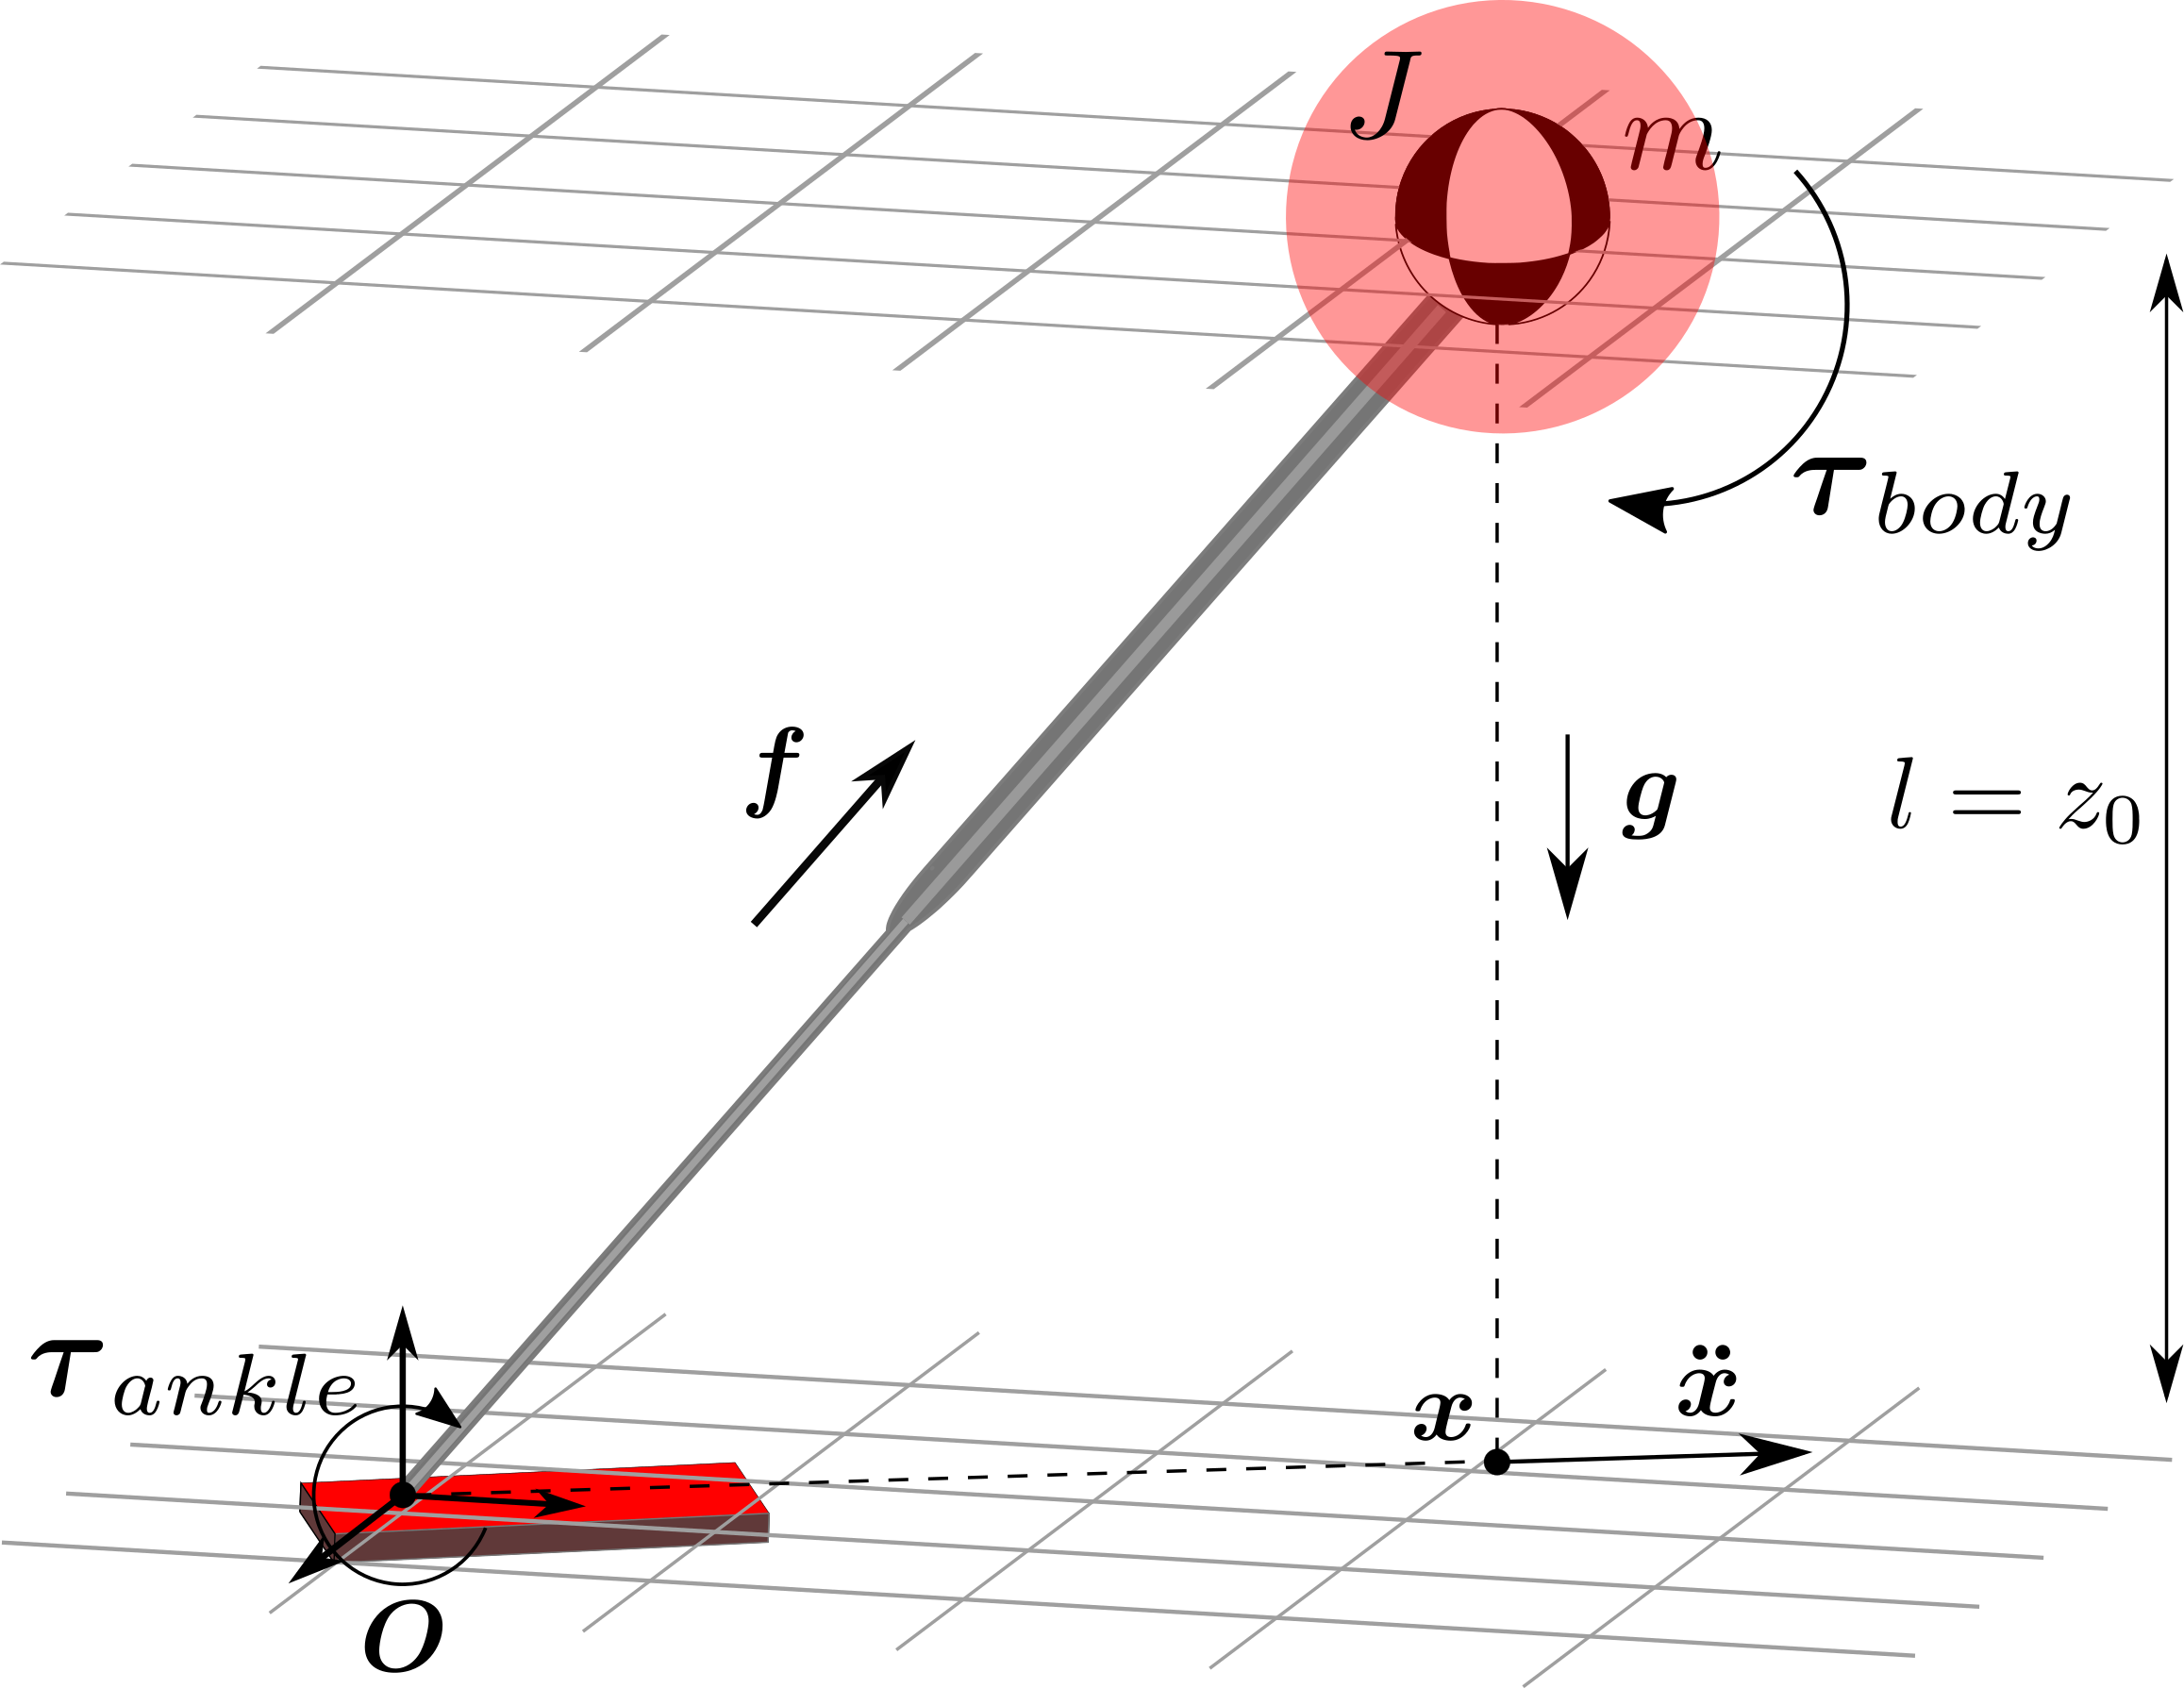
\includegraphics[width=0.5\textwidth]{STYLESTUFF/3DCoMfootinertiaz0.png}
\caption{\ac{3D} motion of \ac{LIP} model with foot at the base and a mass with inertia at the tip. The \ac{CoM} moves at constant height.}
\label{fig:3dlipfootinertiaz0}
\end{figure}





%
% A Real Chapter
\chapter{Background}\label{chap:background}
In this chapter, a brief background is given on legged systems, humanoid robotics at \ac{IHMC} and related works to \ac{CoM} height variation.
% Modeling of Walking
\section{Legged System Preliminaries}
In this section, commonly used expressions and background related to legged systems are briefly presented.
\subsection{Human Balancing Strategies}
As humanoid robots are a derivation of humans, human balancing strategies are briefly discussed. In \figref{fig:human}, balancing strategies are shown for a standing human. The `ankle strategy', `hip strategy' and stepping strategy are most commonly considered as a balancing strategy. However, the figure includes the `suspensory strategy' \cite{hasson1994clinical}, which is less commonly considered. With the `suspensory strategy', the human is in a slightly lower configuration with bent knees to have more control authority of the ankles.

Height variation is often not considered for a standing human. A reason for this might be that the human is often assumed to stand with straight legs. The goal of the `suspensory strategy' however, gives an interesting insight to the problem. Using height changes for balance control, the control authority of the ankles will change. Therefore, height variations for balance control could be a trade-off between the application of additional force and the gain in height. 

For dynamic cases, like walking or jumping, \ac{CoM} height variations for balance on a human can be observed in, for example, the landing after a long jump. Bending the legs and lowering the height is crucial for not falling backwards.
\begin{figure}
\centering
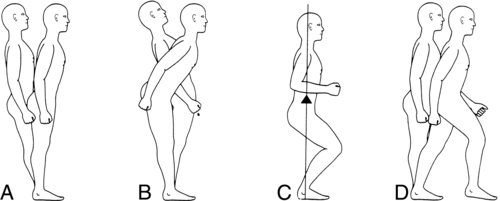
\includegraphics[width=0.5\textwidth]{STYLESTUFF/humanbalance.jpg}
\caption{Balancing strategies for a standing human \cite{hasson1994clinical}. (A) shows the `ankle strategy'. (B) shows the `hip strategy'. (C) shows the `suspensory strategy'. (D) shows the stepping strategy.}
\label{fig:human}
\end{figure}
% Ground Reference Points
\subsection{Ground Reference Points}\label{sec:grp}
In biped locomotion, the dynamics of the system are often simplified by considering the forces resulting from ground contact, the \ac{CoM} location and the angular moment about the \ac{CoM}. The contact forces are commonly summed up in a single \ac{GRF}, coming from a single point of application in the supporting area of the walker. Ground reference points are used to describe the dynamics of the system in a single point, using \ac{GRF} and \ac{CoM} states.

% ZMP
\subsubsection{Zero Moment Point \& Center of Pressure} 
The point on the ground where the resulting \ac{GRF} does not produce any moment in the horizontal plane at the point of application, is referred to as the \ac{ZMP} \cite{sardain2004forces}. By definition, this is the point where the part of the \ac{GRF} that does not cause angular momentum around the \ac{CoM} intersects with the ground surface. The \ac{ZMP} was initially introduced in \cite{vukobratovic1969contribution}. The \ac{ZMP} is formulated as:
\begin{equation}
    \rzmp=\cxy-\frac{\fgrxy}{\fgrz}z+\frac{\taucom}{\fgrz},
\end{equation}
where $\rzmp = [x_{zmp}, y_{zmp}]^T$ is the \ac{ZMP} location, $\fgrxy=[\fgrx,\fgry]^T$ and $\fgrz$ are the horizontal and vertical components of the \ac{GRF} respectively, $\cxy = [x,y]^T$ and $z$ are the horizontal and vertical components of the \ac{CoM} Cartesian position and $\taucom = [-\tau_y,\tau_x]^T$ is the torque about the \ac{CoM} in the horizontal plane. 

In \figref{fig:zmpvscmp} the definition of the \ac{ZMP} is visualized for two different modeling choices, using both a connection between the ankle and the \ac{CoM} as a prismatic joint. In \figref{fig:3dlipfoot}, no inertia is considered around the \ac{CoM} and the \ac{GRF} $\fgr$ coming from the \ac{ZMP} intersect with the mass $m$. The difference in position between the ankle location and the \ac{ZMP} is affected by the ankle torque $\tauankle$. In \figref{fig:3dlipfootinertia}, body inertia of the system is approximated by adding a flywheel with inertia $\inert = [I_x, I_y]^T$ to the model. The \ac{GRF}, coming from the \ac{ZMP}, can be pointed away from the \ac{CoM} by using the body torque $\taucom = [\tau_x, \tau_y]^T$ as input. 

% CoP
The \ac{CoP} coincides during walking over flat ground with the \ac{ZMP} \cite{vukobratovic2004zero}. The two points however are not equal in more complex environments. The \ac{CoP} is restricted to be located in the support polygon, while the \ac{ZMP} is restricted to be located on the ground plane  \cite{sardain2004forces}. Traditionally, the \ac{CoP} is a measured quantity from a force pressure plate under the foot. In this thesis, the \ac{CoP} location is denoted as $\rcop = [x_{cop}, y_{cop}]^T$ and considered equal to $\rzmp$, as a flat contact surface is used as reference.
%The \ac{CoP} is linked to the \ac{GRF}-moment, while the \ac{ZMP} is related to the effects of external forces on the \ac{CoM} state \cite{sardain2004forces}. 
\begin{figure}
\centering
\begin{subfigure}{0.49\textwidth}
\centering
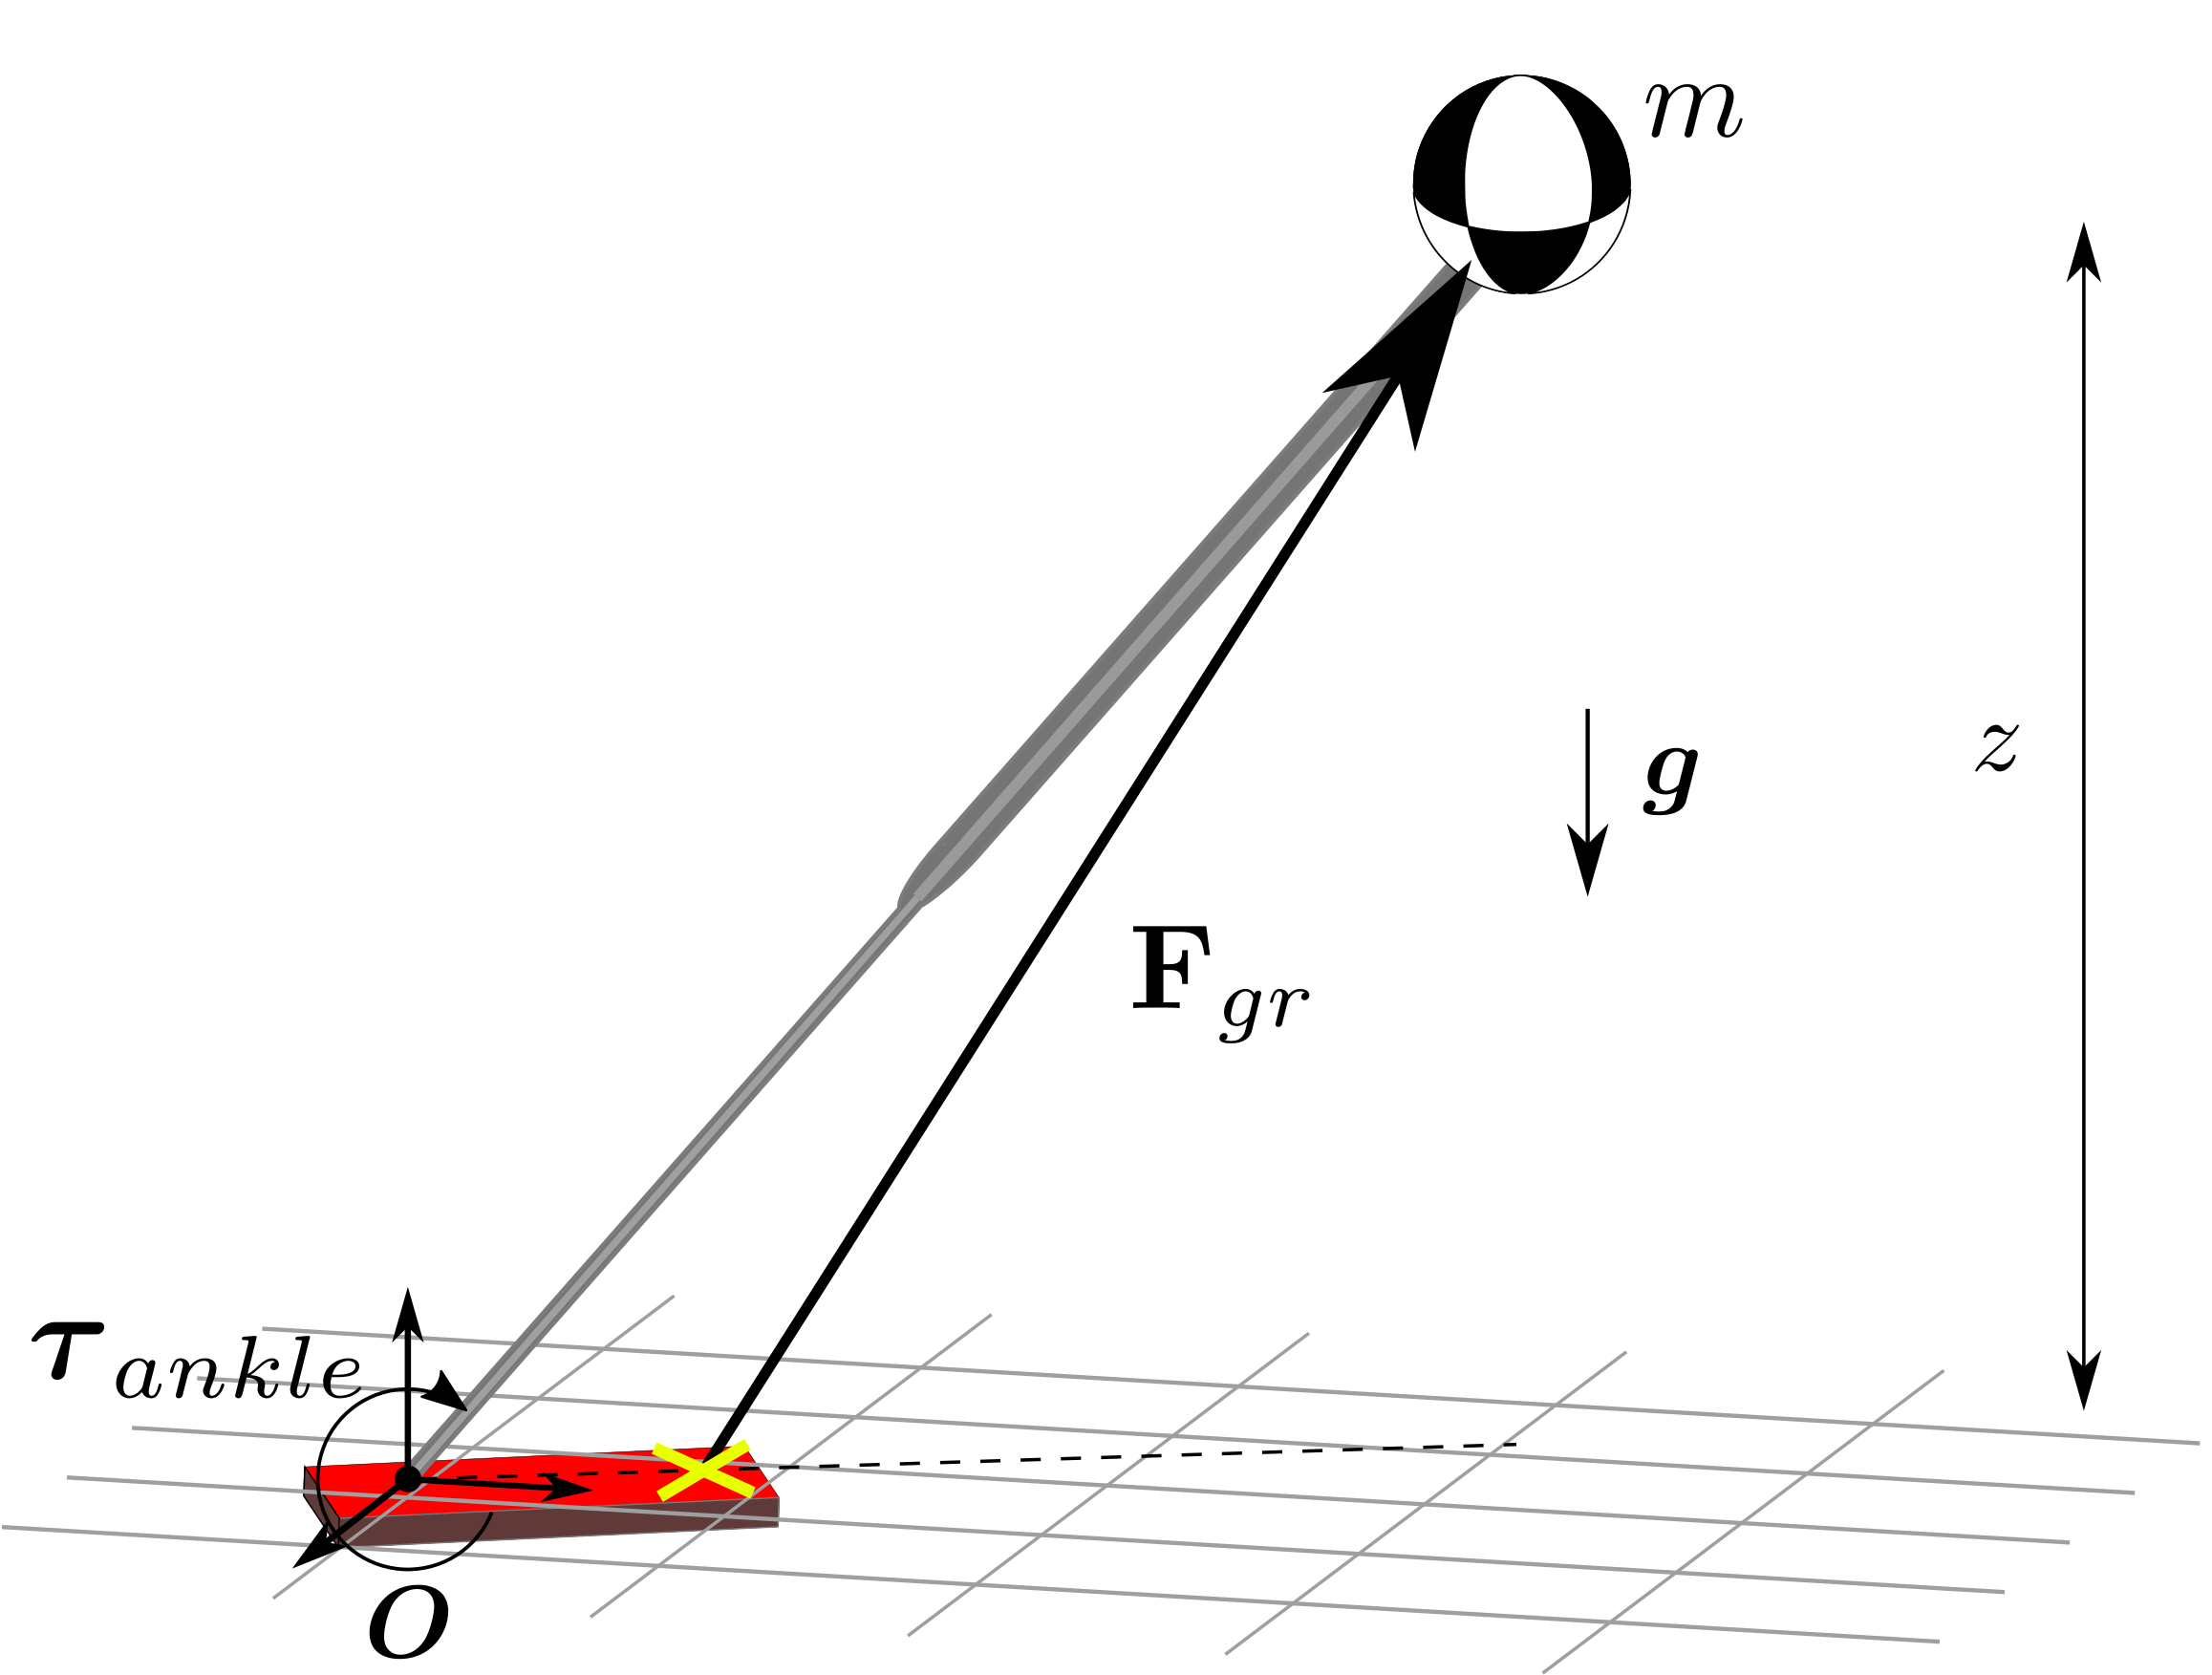
\includegraphics[width=.9\linewidth]{STYLESTUFF/3DCoPviz.png}
\caption{}
\label{fig:3dlipfoot}
\end{subfigure}
\begin{subfigure}{0.49\textwidth}
\centering
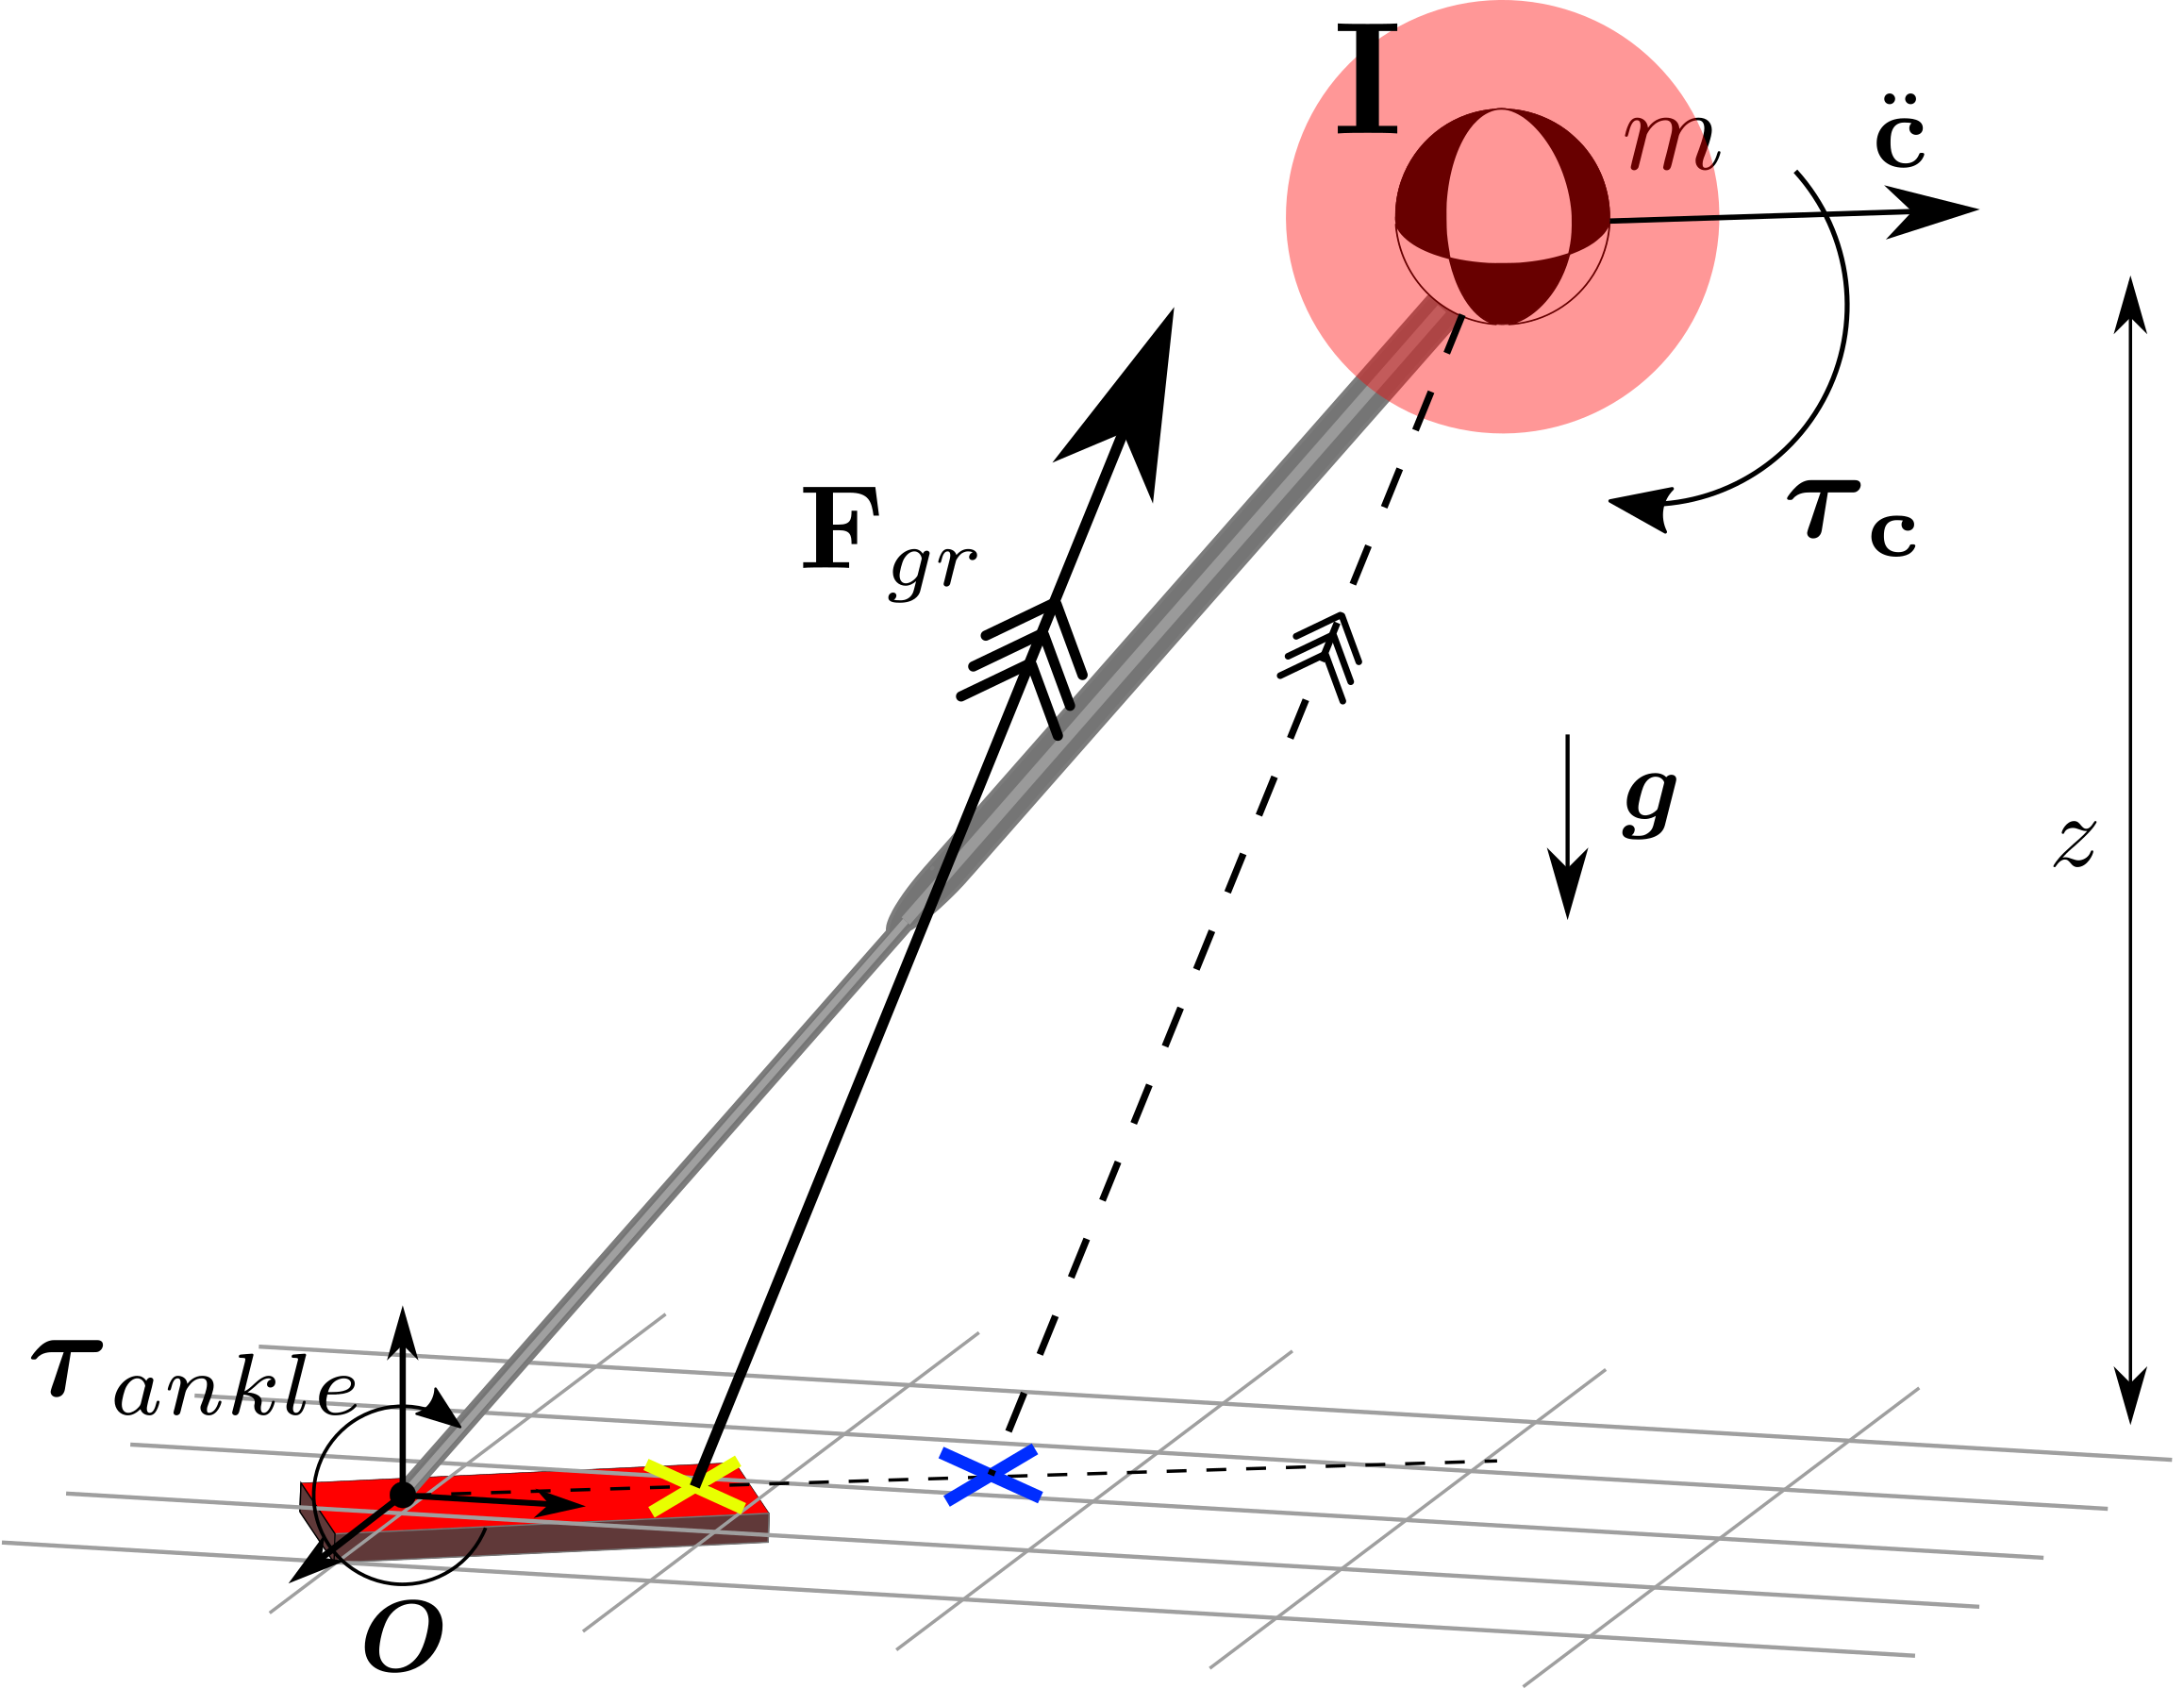
\includegraphics[width=.9\linewidth]{STYLESTUFF/3DCMPCoPviz.png}	
\caption{}
\label{fig:3dlipfootinertia}
\end{subfigure}
\caption{Ground reference points for different modeling choices. (a) The yellow cross points out the \ac{ZMP}/\ac{CoP} location. As no angular momentum is considered in the model,  the yellow cross is also the \ac{CMP}. (b) A flywheel with inertia is added to the model, the blue cross points out the \ac{CMP} location and the yellow cross the \ac{ZMP}/\ac{CoP} location.}
\label{fig:zmpvscmp}
\end{figure}

% CMP
\subsubsection{Centroidal Moment Pivot} 
The \acf{CMP} includes, unlike the \ac{ZMP} and \ac{CoP}, angular momentum about the \ac{CoM}  \cite{popovic2005ground}. This is defined as the point where a line passing through the \ac{CoM}, parallel to the \ac{GRF} intersects with the ground surface. Unlike the \ac{CoP}, the \ac{CMP} is not constrained to lie inside the support polygon. The \ac{CMP} is defined as:
\begin{equation}
    \rcmp=\cxy-\frac{\fgrxy}{\fgrz}z,
    \label{eq:cmp}
\end{equation}
where $\rcmp =[x_{cmp}, y_{cmp}]^T$ is the \ac{CMP} location. In \figref{fig:3dlipfootinertia} the difference between the \ac{ZMP} and \ac{CMP} is graphically explained. Note that without body inertia in the model, the points coincide, as is depicted in \figref{fig:3dlipfoot}. Equivalently, if $\taucom=0$, the points coincide as well.

%leg modeling
\subsection{Inverted Pendulum-based Models}
The line between a ground reference point and the \ac{CoM} can be modeled as an inverted pendulum. In this thesis, this line is also called the \textit{virtual leg}.

\subsubsection{Linear Inverted Pendulum Model} 
For its fast, closed-form solutions, the \ac{LIP} model \cite{kajita20013d} is widely used in walking research and especially in legged robotics. The \ac{LIP} equations of motion are:
\begin{equation}
\ddcxy=\frac{g}{l}\cxy,
\label{eq:LIPeom}
\end{equation}
where $\ddcxy$ is the horizontal \ac{CoM} acceleration. At any horizontal position, a constant leg length is considered and the motion is at a constant height $l=z_0$. In \figref{fig:3dlip} the \ac{3D} motion is visualized if the \ac{CoM} is relatively far from from the base. The pendulum base lies in the origin. Because the \ac{LIP} assumption holds, the vertical component of $\fgr$ cancels out gravity acceleration: $\fgrz=mg$.\\
\begin{figure}
\centering
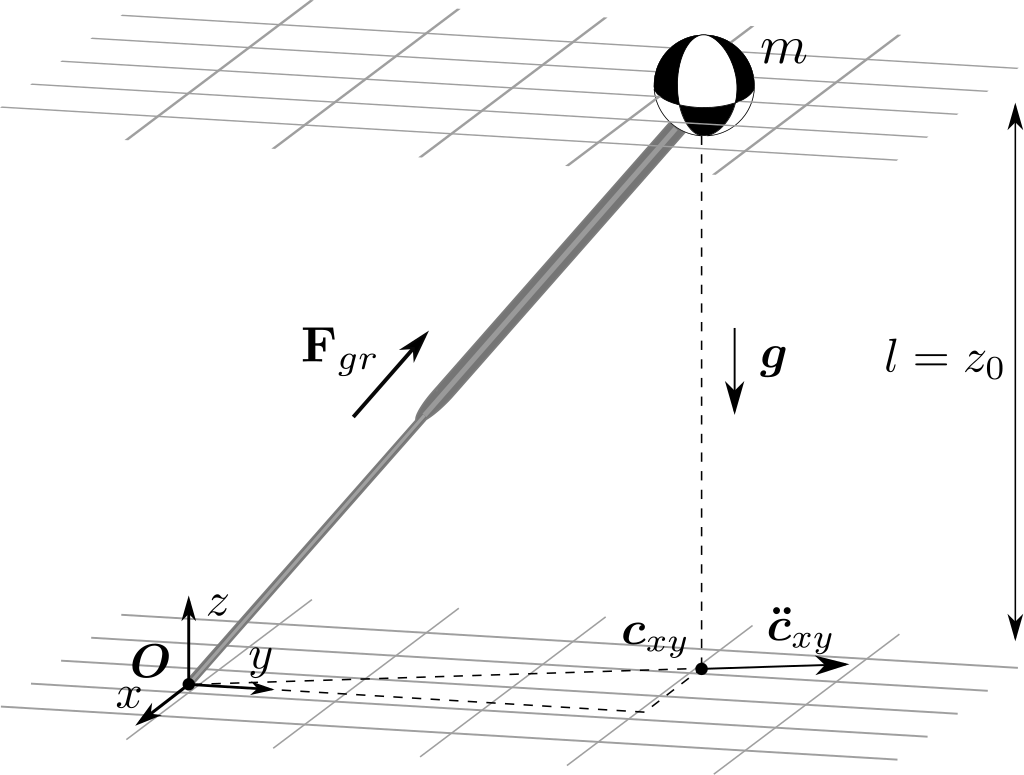
\includegraphics[width=0.5\textwidth]{STYLESTUFF/3DCoMwithoutfoot.png}
\caption{\ac{3D} motion of \ac{LIP} model.}
\label{fig:3dlip}
\end{figure}

To model body inertia of the robot, sometimes a flywheel is added to the \ac{LIP} \cite{pratt2006capture, stephens2007humanoid, koolen2012capturability}. By controlling the torque applied on the flywheel, a control authority  over the \ac{CoM} dynamics becomes available. 

% height var model
\subsubsection{Height Varying Models} 
Unlike the \ac{LIP}, height variation of the \ac{CoM} can be included in modeling of the virtual leg. Three examples of such models are:
\begin{itemize}
	\item The, not linearized, inverted pendulum model \cite{kuo2005energetic};
	\item The \ac{SLIP} model \cite{liu2015trajectory};
	\item A pendulum with prismatic joint, not constrained to maintain a constant height: the \ac{VHIP} \cite{pratt2007derivation}.
\end{itemize}
The inverted pendulum model is often used in human motion research, as in \cite{kuo2005energetic}. The advantages of a \ac{LIP}, like fast, closed-form solutions to the dynamics, are often not needed. The \ac{SLIP} model originates from hopping and running robots \cite{schwind1998spring}. Deviations from the nominal height or pendulum length are modeled as mass-spring dynamics. 

Throughout this report, special focus is given to the \ac{VHIP}. In \figref{fig:3dvhip} the \ac{VHIP} is depicted. The dynamics of the point-mass can be written in two ways. One is as a function of the \ac{GRF} in \ac{2D}:
\begin{align}
	m\ddot{x} &= \fgrtwo\frac{x}{\sqrt{x^2 + z^2}},\\
	m\ddot{z} &= \fgrtwo\frac{z}{\sqrt{x^2 + z^2}} - mg,
	\label{eq:dynamicsprattstyle}
\end{align}
where $\fgrtwo=[\fgrx, \fgrz]^T$ is the \ac{GRF} of the \ac{2D}  model. Works that use this equation are, for example, \cite{pratt2007derivation} and \cite{koolen2016balance}.

Another way of writing the dynamics of the \ac{VHIP} is as a function of the vertical acceleration $\ddot{z}$:
\begin{equation}
	\ddcxyz = \frac{g+\ddot{z}}{z}\cxyz + \vect{g},
	\label{eq:dynamicscaronstyle}
\end{equation}
where $\vect{g}=[0,0,-g]$ is the gravity force vector. The dynamical equation can be seen as a linear time-varying system. Examples of works that use the latter dynamical description for the \ac{VHIP} are \cite{hopkins2014humanoid} and \cite{caron2018balance}. Note that the two models are identical in \ac{2D}.
\begin{figure}
\centering
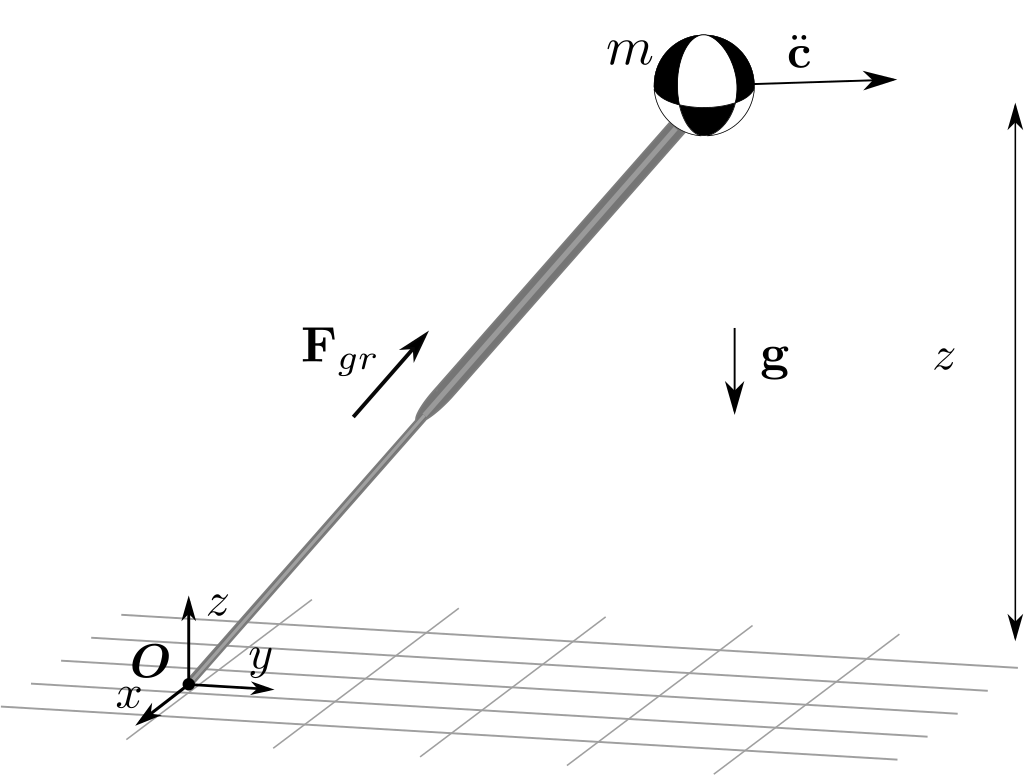
\includegraphics[width=0.5\textwidth]{STYLESTUFF/3DCoMwithoutfootVHIP.png}
\caption{\ac{3D} motion of \ac{VHIP} model.}
\label{fig:3dvhip}
\end{figure}

% Energy of Walking
\subsection{Orbital Energy \& the Capture Problem}\label{sec:ewalking}
An advantage of the \ac{LIP} is that closed-form solutions to the dynamics exists. The \ac{LIP} orbital energy is an example of such a closed-form solution. This energy can be used to determine the ability of the pendulum to converge to its unstable mode: the capture problem \cite{pratt2006capture}, \cite{koolen2012capturability}.

% LIP orbital energy
\subsubsection{Linear Inverted Pendulum Orbital Energy}\label{subsec:liporbit} 
The \ac{LIP} orbital energy is originally derived in \cite{kajita1992dynamic} and shows one of the main advantages of the use of a \ac{LIP} model.  This energy reads as follows
\begin{equation}
\Elip = \int (\ddot{x}-\frac{g}{l}x)\dot{x} dt = \frac{1}{2}\dot{x}^2-\frac{g}{2z_0}x^2,
\label{eq:Elip}
\end{equation}
where $E_{LIP}$ is the \ac{LIP} orbital energy. This orbital energy is a conserved quantity if no contact change occurs. Note that the expression resembles kinetic and potential energy: one term depends on velocity, the other on position. If $E_{LIP}>0$, the point mass will cross the horizontal position of the pendulum base with its current velocity. If $E_{LIP}<0$, the point mass will not cross the pendulum base and will have a turning point where the velocity becomes zero.

% ICP
\subsubsection{Capture Point \& Capture Region} 
More than a decade later than the first mention of the \ac{LIP} orbital energy, the \ac{CP} was presented in  \cite{pratt2006capture}. Taking $E_{LIP}=0$ and taking the square root of Equation \eqref{eq:Elip} gives
\begin{equation}
\xcplip=\sqrt{ \frac{z_0}{g}}\dot{x} 
\label{eq:cp}
\end{equation}
where $\xcplip$ is the `capture point', in this thesis referred to as the \ac{CP}. If the \ac{CoP} is held constant at the \ac{CP}, the velocity of the point-mass will be exactly driven to zero when it is above the \ac{CoP}. In \figref{fig:2dicp} a \ac{2D} visual explanation is given of this point. The \ac{CP} will be used for comparison with the \ac{VHIP} capture regions later in this report.
\begin{figure}
\centering
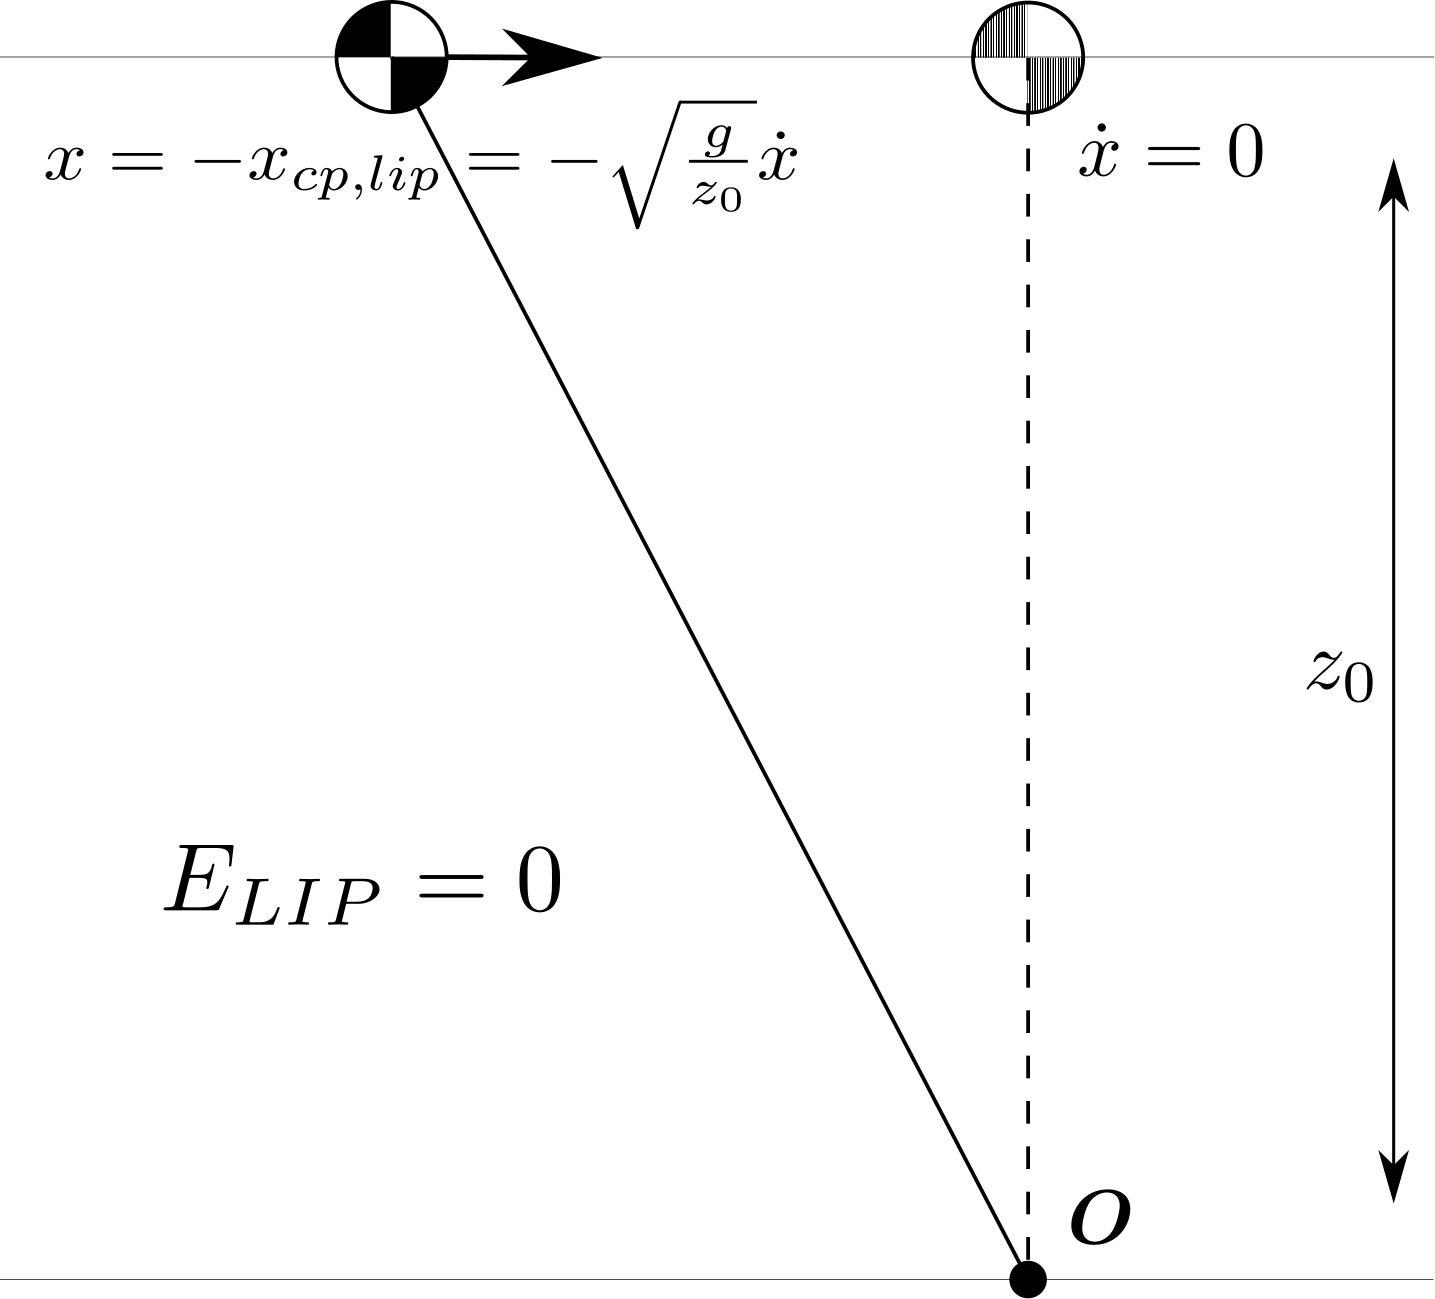
\includegraphics[width=0.4\textwidth]{STYLESTUFF/2DCP.png}
\caption{Visualization of the path to the \ac{CP}. }
\label{fig:2dicp}
\end{figure}

A capture region will traditionally appear if the \ac{LIP} plus flywheel model is used \cite{pratt2006capture, stephens2007humanoid, koolen2012capturability}. As the control authority over the flywheel can change the \ac{CoM} dynamics, a set of capture points become reachable.

\subsubsection{Instantaneous Capture Point} 
The \ac{ICP} was introduced in \cite{koolen2012capturability}, which gives a slightly different description of the \ac{CP}:
\begin{equation}
\icp=\cxy+\sqrt{\frac{z_0}{g}}\dot{\mathbf{c}}_{xy} 
\label{eq:icp}
\end{equation}
where $\icp=[\icpx, \xi_y]^T$ is the \ac{ICP}. In this way, the \ac{CP} is written in environmental coordinates and can be seen as a point where to step in the environment to come to a stop. Other similar mentions to the \ac{ICP} are the extrapolated center of mass \cite{hof2008extrapolated} and the \ac{DCM} \cite{takenaka2009real}. 
\paraskip
For planning and control, the time derivative is often taken of the \ac{ICP}: the \ac{ICP} dynamics \cite{koolen2012capturability}. This time derivative can be written as a function of the current \ac{ICP} location and a ground reference point:
\begin{equation}\label{eq:icpdyn}
\dot{\icp}=\sqrt{ \frac{g}{z_0}}(\icp-\vect{r})
\end{equation}
where $\dot{\icp}$ is the \ac{ICP} velocity and $\vect{r}$ is a ground reference point, depending on modeling choices as discussed in Section \ref{sec:grp}.

% Boundedness
%\paragraph{The boundedness condition}\label{sec:boundedness} \cite{lanari2014boundedness} includes the effects of the motion of the ground reference point in the capture problem. The solution of $x_u$, a point that also coincides with the \ac{ICP}, reads as:
%\begin{equation}
%x_u(t,r) = e^{\omega_0(t-t_0)}x_u(t_0) -\omega_0 \int_{t_0}^t e^{\omega_0(t-\tau)}r(\tau)d \tau,
%\end{equation}
%where $r(t)$ is the trajectory described by the used ground reference point, the virtual base of the pendulum. The boundedness condition reads as follows: if the the future input $r(t)$ results in convergence of the \ac
%{CoM} to the unstable mode, the following equality holds:
%\begin{equation}
%x_u(t_0) = \omega_0 \int_{t_0}^{\infty} e^{-\omega_0(\tau-t_0)}r(\tau)d \tau.
%\end{equation}
%The initial condition, which is equal to the \ac{ICP}, has to be related to $r(t)$ by this expression.

%nonlinear orbital
\subsubsection{Orbital Energy with Height Variation}\label{subsec:nonorbit} 
Allowing height variation of the \ac{CoM}, an expression for orbital energy is more difficult to derive than its linear counterpart.  Examples of attempts to include \ac{CoM} height variations in the solution to the dynamics are the time-varying \ac{DCM} \cite{hopkins2014humanoid}, the orbital energy under a virtual constraint \cite{pratt2007derivation} and the height varying boundedness condition \cite{caron2018balance}. These works are discussed in Section 
\ref{sec:relatedworksheight}, since they are highly related to the research of focus.

% Control Framework IHMC
\section{Humanoid Robotics at IHMC}\label{sec:ihmc}
To support the methods and results presented later in this thesis, this section presents a brief background on humanoid robotics at \ac{IHMC}. Most algorithms are written in Java and simulations are run in \ac{SCS}.
%robots
\subsection{Robots}
There are two humanoid robots present at the institute at the moment of writing: Boston Dynamics' Atlas \cite{koolen2016design}, \cite{kuindersma2016optimization} and NASA's Valkyrie \cite{radford2015valkyrie}. An important difference between the two robots is that Atlas is hydraulically actuated, while Valkyrie relies on electric series elastic actuators. The actuation of Atlas is in general more powerful, which allows the robot to take higher steps. Valkyrie on the other hand, has more precise torque sensing, which is important for torque control on the robot. This ties to a similarity between the robots: both robots are torque controlled. Using a control framework, the actuators of the robots can be controlled using measured and reference torque. In \figref{fig:robots}, the two robots are shown.
\begin{figure}
\centering
  \begin{subfigure}{0.49\textwidth}
  \centering
  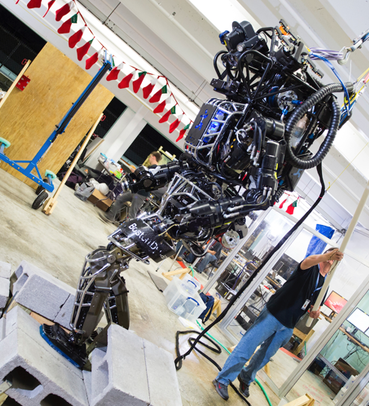
\includegraphics[width=.6\linewidth]{STYLESTUFF/AtlasOld1.png}
   \caption{}
    \label{fig:atlas}
  \end{subfigure}
  \begin{subfigure}{0.49\textwidth}
    \centering
  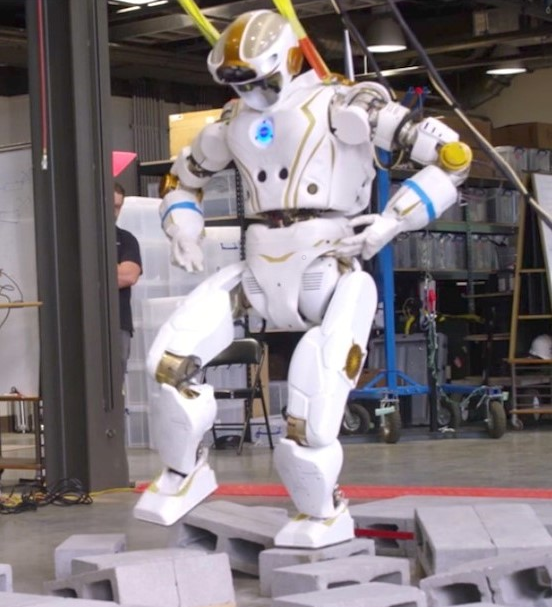
\includegraphics[width=.6\linewidth]{STYLESTUFF/Valkyrie1.png}
  \caption{}
   \label{fig:valkyrie}
  \end{subfigure}
  \caption{(a) Atlas \cite{oldatlas} and (b) Valkyrie \cite{valkyrie} walking over an un-even cinder block field at \ac{IHMC}. }
  \label{fig:robots}
\end{figure}

% planning
\subsection{Planning}
In contrary to running, with walking there is a state in every cycle with two feet in contact with the ground. This is the \ac{DS} state and the state where only one leg is on the ground is the \ac{SS} state. Additionally, other states within either the \ac{DS} or \ac{SS} state are considered, like toe-off in the transition from \ac{DS} to \ac{SS}. In \ac{SS}, the leg in contact with ground is the support leg and the foot taking a step is the swing leg. The transition between those states and the duration in each state play an important role in the generation of a dynamic plan. Planning of the robots motion is conducted by separating footstep planning from dynamic planning. The dynamic plan in this case is an \ac{ICP} reference trajectory \cite{seyde2018inclusion}.
%footstepplan
\subsubsection{Footstep Planning}
Footstep planning is the generation of a sequence of footsteps for the robot to follow. A Light Detection and Ranging sensor on the head of the robot provides terrain information. One way to generate a footstep plan is to let the user define each footstep via a graphical user interface. Via relatively simple algorithmic checks on for example kinematic reachability, the user interface can show whether a footstep is feasible or not. To make this process more autonomous, recently developments have been made in the creation of a footstep planner based on a A* search algorithm. 
%icpplanning
\subsubsection{Instantaneous Capture Point Planning}\label{subsec:icpplan} 
The generation of a dynamic plan for the robot is conducted by computing an \ac{ICP} reference trajectory. This trajectory relies on the solution to the linear differential equation of the \ac{ICP} dynamics of Equation \eqref{eq:icpdyn}:
\begin{equation}\label{eq:icpsol}
	\icp(t)=e^{\omega_0t}(\icp_0- \vect{r}_0) + \vect{r}_0,
\end{equation}
where $\omega_0=\sqrt{\frac{g}{z_0}}$ is the natural frequency of the \ac{LIP} and $\icp_0$ and $\vect{r}_0$ are the initial \ac{ICP} and ground reference point location or the \textit{knot-points}. This equation assumes that the location of the ground reference point is constant. 

Under the assumption of constant ground reference point locations, the ground reference knot-points, multiple methods have been developed over the years and improvements are being made. The most traditional \ac{ICP} reference trajectory is calculated with a single \ac{ZMP} knot-point \cite{englsberger2012integration} for each footstep. For each \ac{ZMP} knot-point, an \ac{ICP} knot-point is computed by integrating the \ac{ICP} dynamics backwards in time from the last footstep to the first. Using Equation \eqref{eq:icpsol}, the local \ac{ICP} reference value can be computed at any time instance within the plan. 

The above mentioned method is extended in \cite{englsberger2014trajectory}, where multiple \ac{CMP} knotpoints per foot are considered and \ac{SS} and \ac{DS} transitions are interpolated using splines. In the most recent improvements, continous \ac{CMP} reference trajectories are used for the generation of the \ac{ICP} trajectory \cite{seyde2018inclusion}. An estimate of the angular momentum generated during the walking motion is incorporated in the generation of the \ac{CMP} reference. At the time of writing, the latter method is the one currently in use at \ac{IHMC}, and which is used for the experiments in Chapter \ref{chap:walking}.
% icp control
\subsection{Instantaneous Capture Point Control}\label{sec:icpcontrol}
Based on a \ac{CMP} and \ac{ICP} reference trajectory, the following proportional control law is used to generate a desired \ac{CMP}:
\begin{equation}
    \rcmpd=\rcmpr + \mathbf{k}_{\xi}(\icp-\icpr),
    \label{eq:rcmpd}
\end{equation}
where $\rcmpd$ is the desired \ac{CMP}, $\rcmpr$ and $\icpr$ are the reference \ac{CMP} and \ac{ICP} from the \ac{ICP} planner respectively and $\mathbf{k}_{\xi}$ is the \ac{ICP} gain. From $\rcmpd$, the desired horizontal linear momentum rate of change is computed:
\begin{equation}\label{eq:dotldxy}
    \dotldxy = \frac{\cxy-\rcmpd}{z_0}mg,
\end{equation}
where $\dotldxy$ is the desired horizontal linear momentum rate of change, which is the desired horizontal force on the \ac{CoM} of the robot. This value is sent to the whole-body \ac{QP}. Note that this value is computed based on the \ac{LIP} equations of motion. 

% momentum control
\subsection{Momentum-Based Whole-body Control}
The desired horizontal linear momentum rate of change $\dotldxy$, the output of \ac{ICP} control, is one of the inputs for the the whole-body \ac{QP}. The whole-body \ac{QP} finds desired joint accelerations and desired \ac{GRF}, which are translated to desired joint torques by a Newton-Euler inverse dynamics algorithm.

%centroidal
\subsubsection{Centroidal Dynamics}
The constraint on the dynamics of the robot in the whole-body \ac{QP} is based on centroidal dynamics \cite{orin2013centroidal}. Centroidal dynamics describe the dynamics on and about the \ac{CoM} of the robot as a result of external forces like gravity and \ac{GRF}. To explain the \ac{CoM} dynamics for the robotic chain of the humanoid, a short introduction is given to joint to end-effector mapping. The mapping between joint velocities and end-effector motion plays a crucial role in any robotic system:
\begin{equation}\label{eq:jacobian}
\matr{T}=\begin{bmatrix}\bs{\omega} \\ \bs{\upsilon} \end{bmatrix} = \matr{J}(\qjnt)\dqjnt \in \mathbb{R}^6,
\end{equation}
where $\dqjnt$ are the joint velocities, $\matr{J}(\qjnt)$ is the Jacobian that maps joint velocities to the end-effector twist $\matr{T}$. The twist consist of the angular velocity $\bs{\omega} \in \mathbb{R}^3$ and the linear velocity $\bs{\upsilon} \in \mathbb{R}^3$. A basis for momentum-based whole-body control is the use of centroidal momentum:
\begin{equation}
\vect{h}=\begin{bmatrix}\vect{k} \\ \vect{l} \end{bmatrix} =\matr{A}(\qjnt)\dqjnt \in \mathbb{R}^6,
\end{equation}
 where $\matr{A}=\matr{I}\matr{J}$ is the inertia matrix $\matr{I}$ times the jacobian. The centroidal momentum $\vect{h}$ consists of the angular part $\vect{k} \in \mathbb{R}^3$ and the linear part $\vect{l} \in \mathbb{R}^3$. The time derivative of the centroidal momentum, the centroidal momentum rate of change, is the constraint on the dynamics of the robot in the \ac{QP} currently in use \cite{koolen2016design}:
\begin{equation}
\dot{\vect{h}}=\begin{bmatrix}\dot{\vect{k}}\\ \dot{\vect{l}} \end{bmatrix} =\matr{A}\ddot{\vect{q}} +\dot{\matr{A}}\dot{\vect{q}} = \matr{W}_g + \sum_i\matr{W}_{gr,i} + \sum_i \matr{W}_{ext,i}, 
\end{equation}
where $\matr{W}_g$ is the gravitational wrench and $\sum_i\matr{W}_{gr,i}$ the wrench exterted by the total \ac{GRF}, as a sum from the wrench at each contact point considered. The other external wrenches $\sum_i \matr{W}_{ext,i}$ can be caused for example by other contacts than ground. These are considered zero in this thesis: $\sum_i \matr{W}_{ext,i}=\vect{0}$.
%qp
\subsubsection{Whole-Body Quadratic Program} 
The whole-body \ac{QP} \cite{koolen2016design} optimizes between momentum rate objectives and motion objectives to find desired joint accelerations and desired \ac{GRF}. The optimization is formulated as follows:
\begin{equation}
\begin{array}{rlcl}
\displaystyle \min_{\bs{\ddot{q}}_d,\bs{\rho}} & \multicolumn{3}{l}{J_{\bs{\dot{h}}_d} + J_{\bs{J}} + J_{\bs{\rho}} + J_{\bs{\ddot{q}}_d} } \\%+ J_p} \\
\textrm{s.t.} & \matr{A}\ddqjntd + \dot{\matr{A}}\dqjnt = \matr{W}_g + \matr{Q}\bs{\rho}+\sum_i\matr{W}_{ext,i}\\
&\displaystyle \bs{\rho}_{min} \leq \bs{\rho}\\
&\ddot{\qjnt}_{min} \leq \ddqjntd \leq \ddot{\qjnt}_{max},
\end{array}
\end{equation}
where $\ddqjntd$ are the desired joint accelerations, $\matr{Q}\bs{\rho} = \sum_i\matr{W}_{gr,i}$ is the basis vector matrix $\matr{Q}$ times the basis vector multipliers $\bs{\rho}$. The basis vector matrix $\matr{Q}$ consists of all basis vectors of the wrench cones from each ground contact point. In \figref{fig:wrenchcone}, the wrench cone for a single ground contact point is visually explained. Currently, there are $4$ ground contact points considered for each foot of the robot.
\begin{figure}
\centering
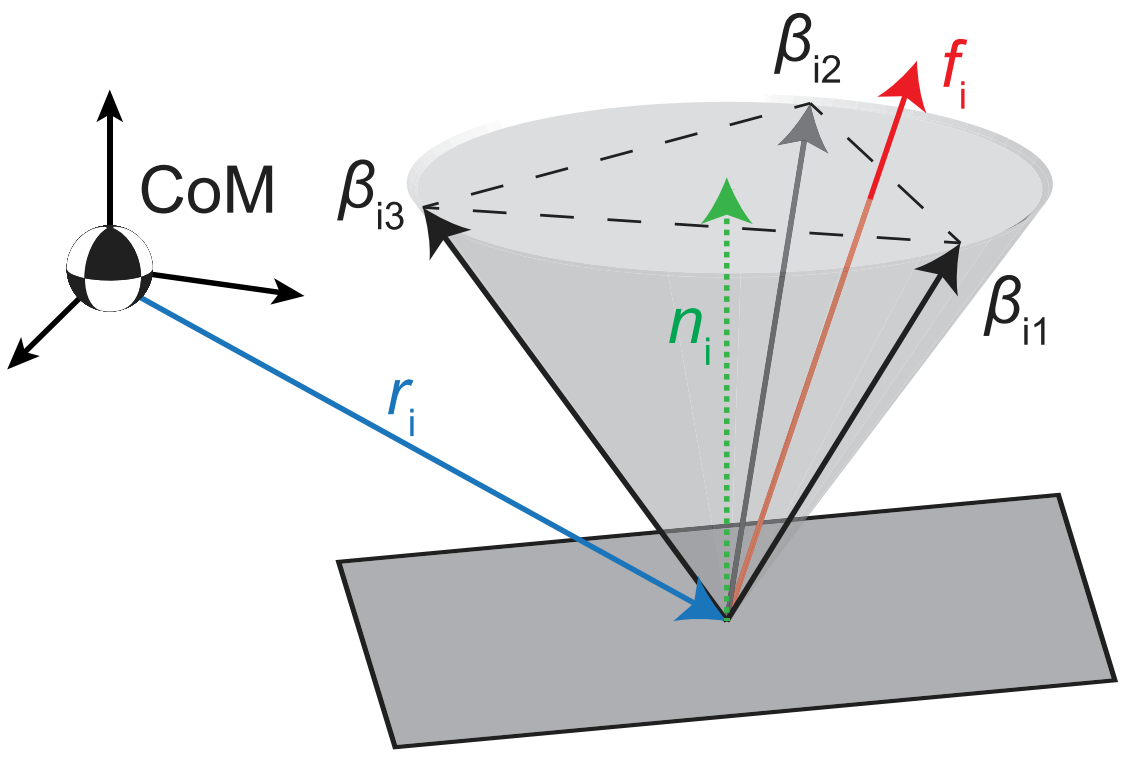
\includegraphics[width=0.4\textwidth]{STYLESTUFF/wrenchcone.png}
\caption{Approximation of the wrench cone with basis vectors $\boldsymbol{\beta}_{ij}$ for ground contact point $i$. The linear part of the ground reaction wrench, $\vect{f}_i$ in the drawing, is a positive multiplication of the basis vectors and lies inside the wrench cone \cite{koolen2016design}. }
\label{fig:wrenchcone}
\end{figure}
The minimum $\bs{\rho}_{min}$ has to be at least zero, because of the unilateral contact constraint; the robot can only push with its feet on the ground. The total cost $J$ is composed of the following cost terms:
\begin{equation*}
\begin{array}{rlcl}
$Momentum rate objective cost:$ & J_{\dot{\vect{h}}_d}= \wght_{\dot{\vect{h}}_d}||\matr{A}\ddqjntd + \dot{\matr{A}}\dqjnt - \dot{\vect{h}}_d||^2\\
$Motion objective cost:$ & J_{\matr{J}_m} = \wght_{\matr{J}_m}||\matr{J}_m\ddqjntd-\vect{p}||^2\\
$Contact force cost:$ & J_{\bs{\rho}}=\wght_{\bs{\rho}}||\bs{\rho}||^2 \\
$Joint acceleration cost:$ & J_{\ddqjntd} = \wght_{\ddqjntd}||\ddqjntd ||^2 \\
%$Privileged configuration cost:$ & J_p = \wght_p||(\matr{I} - \matr{J}_t^{\dagger}\matr{J}_t)\ddqjntd - \ddqjntp||^2,
\end{array}
\end{equation*}
where the weighting terms $\wght$ can have a selecting function as well. For example, the centroidal momentum rate of change objective $J_{\dot{\vect{h}}_d}$ only consists of the linear part and is only affected by the desired linear momentum rate of change $\dotld$. The motion task jacobian $\matr{J}_m = [\matr{J}_1^T\quad...\quad\matr{J}_N^T]^T$ consists of all concatenated jacobians that map either joint acceleration to end-effector motion, as in Equation \eqref{eq:jacobian} or joint acceleration to joint acceleration. The motion objective vector $\vect{p} = [\vect{p}_1^T\quad...\quad\vect{p}_N^T]^T$  consists of PD-controlled desired accelerations, coming for example from trajectory tracking of the swing leg or maintaining the upper-body orientation. %The last cost term $J_p$ is determined by the privileged joint accelerations $\ddqjntp$. Here is $\matr{J}_t$ the all-task jacobian consisting of both the momentum rate objective, as well as the motion objectives. The damped Moore-Penrose pseudo-inverse  $\matr{J}_t^{\dagger} = \matr{J}_t^T(\matr{J}_t\matr{J}_t^T +\mu^2)^{-1}$ with $\mu>0$ is used in the null-space projector $(\matr{I} - \matr{J}_t^{\dagger}\matr{J}_t)$, which projects the priviliged acceleration objective in the null-space of the primary task jacobian $\matr{J}_t$. This can for example be used in singularity avoidance, where the priviliged accelerations are used to determine the configurarion of the robotic chain.  

An important note considering the research of focus is the generation of vertical \ac{CoM} motion of the robot. The desired linear momentum rate of change $\dotld$ consists, next to its horizontal component of Equation \eqref{eq:dotldxy}, of a vertical part:
\begin{equation}
\dotldz =m(k_p(z_r-z) - k_d\dot{z}), 
\label{eq:defaultheightcontrol}
\end{equation}
where $k_p, k_d$ are the PD-control gains and $z_r$ is the reference height coming from a reference trajectory. Decision variables for this trajectory are for example kinematic reachability and height changes in terrain, but maintaining the robot's balance is \textit{not} a part of those decision variables.


\subsubsection{Inverse Dynamics} 
To translate desired joint accelerations and end-effector wrenches to desired joint torques, a recursive Newton-Euler inverse dynamics algorithm is used. Desired joint torques $\bs{\tau}_d$ are calculated using the solution of whole-body \ac{QP}, $\ddqjntd$ and $\bs{\rho}$, as follows:
\begin{equation}
    \bs{\tau}_d = \matr{M}(\qjnt)\ddqjntd + \matr{C}(\qjnt,\dqjnt)\dqjnt + \matr{G}(\qjnt) + \matr{J}^T \vect{W}_{gr}.
\end{equation}
These desired joint torques are used by the torque controllers for each actuator.

A high-level overview of the control framework is shown in \figref{fig:framework}. The `high level controller' block consists for example of the \ac{ICP} controller of Section \ref{sec:icpcontrol} and the height control law of Equation \eqref{eq:defaultheightcontrol}.
\begin{figure}[h]
\centering
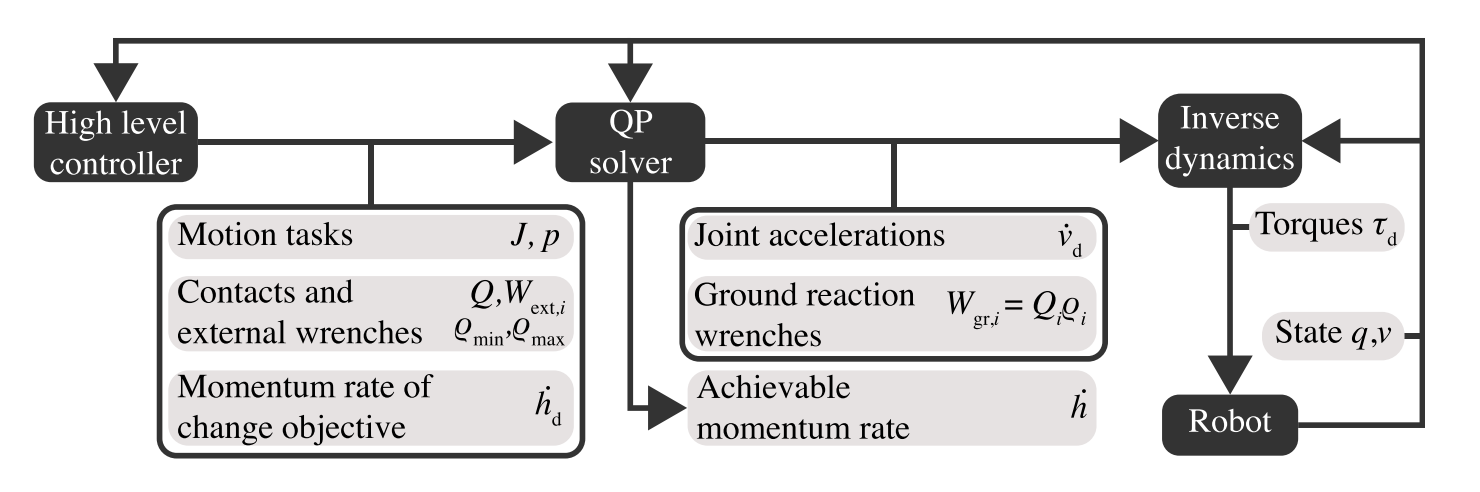
\includegraphics[width=0.8\textwidth]{STYLESTUFF/controlframework.png}
\caption{High-level overview of the control framework \cite{koolen2016design}. }
\label{fig:framework}
\end{figure}

% CoM Height Variation
\section{Related Work}\label{sec:relatedworksheight}
In this short literature survey, the scope is not limited to only the use of vertical \ac{CoM} motion in balance control. Other goals of improvement, like improving dynamic planning for motions over rough-terrain or for more human-like motions, are discussed as well. The models and strategies used in these works can be insightful for the problem considered in this thesis.

Traditionally, vertical \ac{CoM} motion is generated through PD-control as in Equation \eqref{eq:defaultheightcontrol} \cite{kajita2003resolved, koolen2016design}: a dynamic reference plan exists, often based on the LIP model, and height variations are considered as disturbances on the model considered in the dynamical plan. Reasons to use height variations here include the guarantee of \textit{kinematic feasibility}: height variation allows the robot to step up platforms, and allows the robot to take larger steps. A noteworthy, more unique, example of height variation in non-predictive control is walking with straighter legs as in \cite{griffin2018straight}. The motivation in this work is to let the robot walk more \textit{human-like}, which could have more underlying benefits, such as kinematic reachability and metabolic energy consumption \cite{wang2012optimizing}.

%var height terrain
\subsection{Dynamic Planning \& Walking Pattern Generation}
Because the constant height assumption of the \ac{LIP} is constraining the dynamics of the robotic system, efforts have been made to incorporate CoM height variation in the generation of a dynamic plan. Instead of using a LIP model, a more complicated model is used. \textit{Expected} height variations of the CoM can be incorporated in the dynamic planning problem, which improves the \textit{dynamic feasibility} of the plan. In theory, the reference dynamics are closer to the real dynamics of the robot. Deviations from the \ac{LIP} in the \ac{CoM} reference can be incorporated in the plan. These deviations can come for example from an un-even terrain, or a human-like walking pattern.

An example of incorporating height variations in terrain in the dynamic planning problem can be found in \cite{englsberger2013three}, which is an extension of \ac{ICP} planning as in Section \ref{subsec:icpplan}. Additional reference points, similar to ground reference points as in Section \ref{sec:grp}, are designed and used in the planning method. The drawback of this method is that still a linearized model is considered and the trajectories between footsteps for the dynamical plan are constrained to be straight lines. 

Another work improved this latter aspect by introducing the time-varying \ac{DCM} \cite{hopkins2014humanoid}. The natural frequency of the \ac{LIP} was made time-varying, such that the \ac{DCM} became time-varying. However, a closed-form solution using this method was not available anymore and a dynamic plan was computed numerically.

The methods presented in \cite{brasseur2015robust} and \cite{kajita2017biped} also show the objectives of walking with straighter legs in the dynamic planning problem. The objective in the optimization in \cite{brasseur2015robust} is to let the robot walk with the straightest legs as possible at any time. In \cite{kajita2017biped}, a \ac{2D} walking pattern is generated for walking with straighter legs. The third dimension is added, under the assumption that the dynamics in the sagittal plane and the coronal plane can be decoupled. 
%balance
\subsection{Balance Control}\label{subsec:heightbalance}
A very recent objective is the specific use of \ac{CoM} height variation in \textit{balance control}. Traditional balance control strategies are taking a step, movement of the \ac{CoP}, also known as `ankle strategies' and, to a lesser extent, changing the angular momentum about the \ac{CoM}, for example: `hip strategies'. Recently, efforts have been made to incorporate vertical \ac{CoM} motions as an additional strategy for balance control. This is the research of focus in this report.

In this section, the following three publications that consider height variations as control input for balance are discussed. The work proposed by: Koolen, Posa \& Tedrake in \cite{koolen2016balance},  Gao, Jia \& Fu in \cite{gao2017increase} and  Caron \& Mallein in \cite{caron2018balance}:

% 2D polynomial
\paragraph{Koolen et al.} propose a \ac{2D} \ac{MPC} law, based on the \ac{VHIP} orbital energy proposed in \cite{pratt2007derivation}. This energy reads as follows:
\begin{equation}\label{eq:evhip}
    E_{VHIP}  = \frac{1}{2}\dot{x}^2\bar{f}^2(x)+gx^2f(x) - 3g\int_{x_f}^{x} f(\xi)\xi d\xi = \frac{1}{2}\dot{x}_f^2\bar{f}^2(x_f)+gx_f^2f(x_f),
\end{equation}
where $E_{VHIP}$ is the \ac{VHIP} orbital energy. The virtual constraint $z=f(x)$ is used to make a closed-form solution possible for the energy. Furthermore, $\bar{f}(x)=f(x)-f'(x)x$. Unlike its \ac{LIP} cousin, this \ac{2D} orbital energy allows for \ac{CoM} height variation. Note that filling in a constant value for the function, $f(x)=z_0$, rewrites to the \ac{LIP} orbital energy.

The function $f(x)$ is constrained to be a cubic polynomial by Koolen et al. in \cite{koolen2016balance}. Using this description, four constraints are presented, which are used in a matrix to solve for the polynomial constants. There is one constraint on the final height, one constraint on the initial height, one on the initial direction and one constraint on conservation of $E_{VHIP}$. The final position of the polynomial trajectory is above the \ac{CoP} and the final velocity is zero, such that the resulting polynomial trajectory is a \textit{capture trajectory}. 

Similar to the capture regions of \cite{pratt2006capture}, \textit{regions of attraction} for this controller are investigated: initial states in which this controller is still able to let the \ac{VHIP} converge to the unstable equilibrium. However, there are no kinematic constraints taken into account, such that the polynomial trajectories can become unrealistically high above the ground. Though, the analytic solution for the capture trajectory guarantees fast computation times, which allow for the use in \ac{MPC}.

\paragraph{Gao et al.} present different \ac{2D} multi-step strategies to use vertical motion in balance control in \cite{gao2017increase}. An example is the lowering of the \ac{CoM} height in the current step, to exert more force and raise the \ac{CoM} in the next step. In this way, the pendulum can stop closer to the current position than with a \ac{LIP} trajectory. Furthermore, the natural frequency of the \ac{LIP} is adjusted for the added vertical acceleration. To make the dynamical model closed-form solvable over time, a constant height is considered, as the deviations from the initial height are considered as relatively small.

% boundedness
\paragraph{Caron \& Mallein} propose a \ac{3D} \ac{MPC} law in \cite{caron2018balance}, based on a height varying version of the boundedness condition from \cite{lanari2014boundedness}. In \cite{lanari2014boundedness}, the boundedness condition is based on the \ac{LIP} and presents a similar expression as the \ac{ICP}, but takes a time-varying ground reference point trajectory into account.  By using a time varying natural frequency of the pendulum $\omega(t)$, Caron \& Mallein combine the boundedness condition with the time-varying \ac{DCM} of \cite{hopkins2014humanoid}. By the nonlinearity of the problem, it is initially hard to solve real-time. The problem function is reformulated and written as a function of an inverse of time, rather than as a function of time. Also, the capture trajectory is divided in $10$ segments, which are considered to have a piece-wise time-invariant natural frequency. The resulting problem is solved using a nonlinear solver.

This work is expanded in \cite{caron2018capturability}. The problem is extended from `0-step' capture problems to multi-step problems. The problem formulation is rewritten and sequential quadratic programming is used to allow for fast computation times, which makes the multi-step problem solvable real time.

\subsection{Discussion}
The related works show that the use of \ac{CoM} height variations in dynamic planning is a relatively longer existing research than the use of  vertical \ac{CoM} motion in balance control. However, the difference between dynamic planning and \ac{MPC} can be small. The most notable difference between the two is that with \ac{MPC} replanning is conducted every control tick, while with dynamic planning this happens fewer times. Replanning every control tick allows to adjust the dynamic plan for disturbances applied on the system. The similarity between the two is that, in the works mentioned, both use a \ac{VHIP} or an adjusted \ac{LIP} model for computing the predicted dynamics of the system.

When going from the \ac{LIP} to the \ac{VHIP}, the problem arises of losing the explicit solution to the dynamics. To avoid large computation times due to numerical integration, in the works related to balance control constraints are introduced to allow for faster solutions. More specifically, Koolen et al. constrain the \ac{2D} vertical position of the \ac{VHIP} to be a cubic polynomial function of its horizontal position. Gao et al. consider an adjusted constant natural frequency for the \ac{LIP} model to account for vertical acceleration. Caron et al. use piece-wise time-invariant natural frequencies to obtain fast solutions. Furthermore, the kinematic constraints of the robot, such as a maximum leg length, are approximated with a minimum and maximum \ac{CoM} height.

Also, the works present no application of the controllers in a control framework to control humanoid robots. Therefore, the question remains what the advantages are of the presented \ac{MPC} law compared to using a \ac{LIP}-based proportional controller for example. In Chapter \ref{chap:standing} and Chapter \ref{chap:walking} of this report, \ac{CoM} height variations in balance control are compared with constant height approaches on humanoid robots.

Comparable with the \ac{LIP}-based `capture regions' in \cite{pratt2006capture}, \cite{koolen2012capturability} and `stable regions' \cite{stephens2007humanoid},  Koolen et al. investigate `regions of attraction' for the unconstrained \ac{VHIP} orbital energy trajectories. Traditional `capture regions' consider inertia about the \ac{CoM} to control the \ac{CP}. The \ac{VHIP} `regions of attraction' use \ac{CoM} height variation as a control input. The `regions of attraction' show an interesting insight in capture regions of the \ac{VHIP} model. However, only a constraint of contact unilaterality is considered and no additional constraints are introduced to take kinematic and torque limits of the robot into account. Also, the trajectory cannot have any desired shape and is constrained by the polynomial function.

In the next chapter, capture regions are presented for the \ac{VHIP} model, by considering additional constraints. Like in the approach of Caron et al., constraints on the kinematics and dynamics of the system are approximated with a constraint on vertical position and acceleration.
%
% Another appendix chapter
\chapter{Theoretic Limits on Capture}
It is hard, or even impossible, to find a closed-form solution of the state of a time-varying or nonlinear inverted pendulum model forward in time without introducing additional constraints, as discussed in Section \ref{sec:ewalking}. A common approach is to formulate an optimization problem, as for example in \cite{caron2018capturability}, to come to capture trajectory. However, few methods mention the limits achievable of the underlying model of the optimization problem. As convergence is often a problem in constrained nonlinear optimization, it could be useful to have a good guess of which states are achievable and which are not. In this chapter, limits on capture are given, considering constraints on height. As with the \ac{CP}, a point-foot, point-mass model is considered. Important constraints for this model are:
\begin{itemize}
	\item Unilateral \ac{GRF}.
	\item Limit on leg length or height.
	\item Limit on leg force.
	\item Limit on ground friction.
\end{itemize}
The latter two constraints are not considered in the following methods and therefore are the introduced points seen as limits or approximated effects, as they are likely not achievable with the true system.

 %% Capture Region
\section{Unconstrained Capture Region}
The search for the the new points is started off by finding a limit only under constraint of unilaterality of \ac{GRF}. Like with \ac{CP}, an initially horizontally traveling point-mass is considered. \\
The balistic touchdown time for a given height is for this point-mass:
\begin{equation}\label{eq:tbal}
	t_{balistic} = \sqrt{\frac{2z_0}{g}}.
\end{equation}
The horizontal touchdown location is:
\begin{equation}
	x_{balistic}= \dot{x}t=\dot{x}\sqrt{\frac{2z_0}{g}} 
\end{equation}
which is compares to the capture point as:
\begin{equation}
    x_{balistic}=\sqrt{2}x_{cp}
\end{equation}
This can also be reasoned from a leg force perspective, as no energy is substracted from the point-mass during its travel. Using this formulation and inserting a final velocity Equation \eqref{eq:Elip} gives:
\begin{equation}
   x_{balistic}^2 = \frac{z_0}{g}(\dot{x}_0^2 + \dot{x}_f^2), 
\end{equation}
where $\dot{x}_f$ is the final horizontal velocity of the \ac{CoM}. If a balistic trajectory is considered, the horizontal velocity is not affected until touchdown, so $\dot{x}_0=\dot{x}_f$. \\
To explain this with respect to a limit on the capture region: at thouchdown, the virtual leg can apply an impuls so that $\dot{x}_f$ becomes zero. After this, the point-mass can be risen to its original height again, without influencing the horizontal dynamics, which are zero. On the other side of the region, when to point-foot position is infinitely close to the point-mass, the virtual leg has to apply an infinite force to let the horizontal velocity become zero. After this, the point-mass can be lowered again to its default height. The region of between those two limits reads as follows:
\begin{equation}
\{x_{\dot{x}_f=0} \in (0, \dot{x}\sqrt{\frac{2z_0}{g}} ]\}.
\end{equation}
In \figref{fig:cpbal} this region and how this compares to the \ac{CP} is visualized. With grey plots, made with the method of \cite{koolen2016balance}, it can be observed how the trajectories can evolve approaching the limits. 

\begin{figure}[h]
\centering
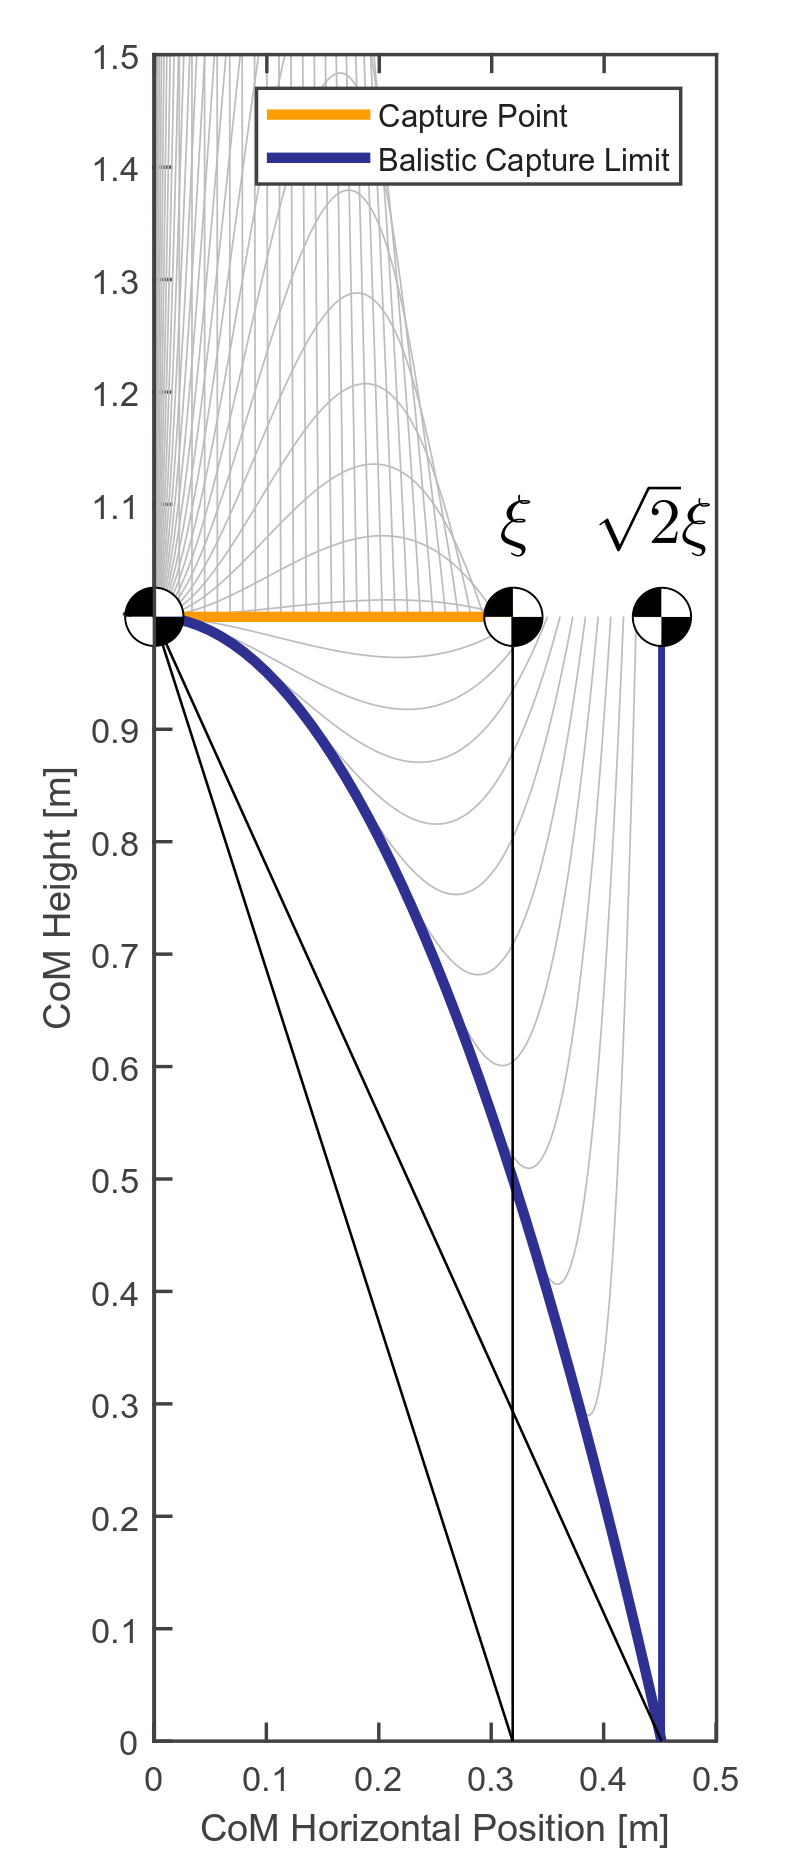
\includegraphics[width=0.3\textwidth]{STYLESTUFF/CPvsBalistic.png}
\caption{Unconstrained capture region and balistic limit. The grey plots visualize possible intermediate trajectories and are made with the method of \cite{koolen2016balance}}.
\label{fig:cpbal}
\end{figure}
\newpage
%% Impact influence
\section{Impact Influenced Capture}
To find the influence of the impact on capture, the question of the previous section is reversed: what does an nonzero negative height velocity do to the capturability, if it is directly stopped by an impact? To some extend, this has similarities to the work done in \cite{kuo2005energetic}. In the mentioned work, one of the goals is to find the energetic effects of the impacts of steps when a (nonlinear) inverted pendulum model is considered. In this section, the energetic influences are considered by direct trantioning to the \ac{CP} trajectory.\\
Consider a capture point where the initial horizontal velocity is increased by an impact:
\begin{equation}
x_{cp,impact} = \sqrt{\frac{z}{g}}(\dot{x}_0+\dot{x}_I),
\end{equation}
where $x_{cp,impact}$ is the impact influenced capture point and $\dot{x}_I$ is the added velocity generated by an impact. In the same way as in \eqref{eq:dotximpact}, this added velocity in terms of vertical velocity is written as:
\begin{equation}
x_{cp,impact} = \sqrt{\frac{z_0}{g}}(\dot{x}_0-\frac{x_{cp,impact}}{z_0}\dot{z}_I). 
\end{equation}
Under the assumption that the vertical velocity is driven to zero instantaneously by the impact, $\dot{z}_I=-\dot{z}_0$. Again, writing this point not as a function of itself, leads to:
\begin{align}\label{eq:xcpimpact}
x_{cp,impact} &= \frac{\sqrt{\frac{z_0}{g}}}{1+\frac{\dot{z}_I}{z_0}\sqrt{\frac{z_0}{g}}}\dot{x}_0,\\
			&= \frac{z_0}{\sqrt{z_0g}-\dot{z}_0}\dot{x}_0.
\end{align}

%% Height Constrained
\section{Height Constrained Capture}
If a time-varying model is considered for the capture point as in \cite{hopkins2014humanoid}, no closed form solution is possible. However, under the assumption that all height changes of the point-mass are generated by an initial impact generated by the virtual leg, the closed form solution is available. If this impact is either as early or as late as possible under the considered height constraint, it is a limit on capture for that particular height constraint. The more leg force is used farther from the virtual foot in horizontal direction, the more effect it has on the horizontal dynamics (Equation \eqref{eq:LIPeom}).\\
%minheight
\subsection{Minimum Height}
To calculate the limit under a minimum height constraint $z_{min}$, the point-mass has to fall until the constraint is reached, since the later the force is applied, the closer the point-mass is at its virtual base and the farther the mass can reach. Deriving from \ref{eq:tbal}, the balistic trajectory until the minimum height has as final height velocity:
\begin{equation}
	\dot{z}_{zmin} = -gt_{bal,z_{min}} = -g\sqrt{\frac{2\delta_{zmin}}{g}} = -\sqrt{2g\delta_{zmin}},
\end{equation}
where $t_{bal,zmin}, \dot{z}_{zmin}$ are the time and height velocity at the minimum height constraint and $\delta_{zmin}=z_0-z_{min}$. Plugging this height velocity in the impact influenced capture point of Equation \eqref{eq:xcpimpact} brings:
\begin{equation}
	x_{cp,impact}(z_{min}, \dot{z}_{zmin})= \frac{z_0-\delta_{zmin}}{\sqrt{(z_0-\delta_{zmin})g}+\sqrt{2g\delta_{zmin}}}\dot{x}_0.
\end{equation}
The capture point under a minimum height constraint is:
\begin{equation}
	x_{cp,minheight} =x_{bal,zmin}+x_{cp,impact}(z_{min}, \dot{z}_{zmin}) ,
\end{equation}
where  $x_{bal,zmin}$ is the horizontal position at the end of the balistic part. This results in the following equation for the capture limit under the minimum height constraint:
\begin{equation}
 x_{cp,minheight}=(\sqrt{\frac{2\delta_{zmin}}{g}} +\frac{z_0-\delta_{zmin}}{\sqrt{(z_0-\delta_{zmin})g}+\sqrt{2g\delta_{zmin}}})\dot{x}_0.
\end{equation}
In \figref{fig:cpzmin} the trajectory to this point is visualized.
%maxheight
\subsection{Maximum Height}
To calculate the initial impact as a function of the maximum height, there is looked at a simple kinetic and potential energy formula:
\begin{align}
 	\frac{1}{2}m\dot{z}_I^2 &= mg\delta z_{max},\\
 	\dot{z}_I &= \sqrt{2g\delta z_{max}},
\end{align}
where $\dot{z}_I$ is the generated vertical velocity by the impact and $\delta z_{max}$ is the height difference between the current and the maximum height, considering the initial vertical velocity is zero, as with the \ac{CP} \cite{pratt2006capture}. The initial horizontal velocity is influenced at the moment of impact as:
\begin{equation}\label{eq:dotximpact}
	\dot{x}_{0,I} = \dot{x}_0-\frac{x_{cp,height}}{z_0}\dot{z}_I,
\end{equation}
where $\dot{x}_{0,I}$ is the remaining horizontal velocity after impact and $x_{cp,height}$ is the capture point under the height constraint, to be determined. The way the height velocity $\dot{z}_I$ is calculated, assumes no external forces except for gravity $g$ in its calculation. As such, if the virtual leg would excert force during the time the vertical velocity after the impact $\dot{z}$ is nonzero, the height constraint $z_{max}$ would be violated. During the time $\dot{z}$ is driven to zero by gravity, the virtual leg force is considered to be zero. Under the motivation to find a limit on the closest possible point to come to a stop, the \ac{CP} is considered after the horizontal position where the $\dot{z}$ is driven to zero. In this way, the maximum leg force possible is used without violating the constraint $z_{max}$. Note that at the moment when $\dot{z}$ is zero, $\dot{x}_{0,I}$ is still the same value as just after the impact.\\
The time it takes until $\dot{z}$ is zero after the impact with zero leg force, is given by:
\begin{equation}
	t_{\dot{z}} =\frac{\dot{z}_I}{g},
\end{equation}
where $t_{\dot{z}}$ is the time that the height velocity is nonzero. With the proposed strategy, the capture point under maximum height constraint can be calculated the following way:
\begin{align}
	x_{cp,height}&=(t_{\dot{z}}+\sqrt{\frac{z_o+\delta z_{max}}{g}})\dot{x}_{0,I},\\
			&=(\frac{\dot{z}_I}{g}+\sqrt{\frac{z_o+\delta z_{max}}{g}})(\dot{x}_0-\frac{x_{cp,height}}{z_0}\dot{z}_I),
\end{align}
where $x_{cp,height}$ is the capture point under the constraint of $z_{max}$. Writing this expression not as a function of itself, leads to:
\begin{align}
	 (1+(\frac{\dot{z}_I}{g}+\sqrt{\frac{z_o+\delta z_{max}}{g}})\frac{\dot{z}_I}{z_0})x_{cp,height}& =		(\frac{\dot{z}_I}{g}+\sqrt{\frac{z_o+\delta z_{max}}{g}})\dot{x}_0,\\
	 x_{cp,height} & = \frac{(\frac{\dot{z}_I}{g}+\sqrt{\frac{z_o+\delta z_{max}}{g}})\dot{x}_0}{ 1+(\frac{\dot{z}_I}{g}+\sqrt{\frac{z_o+\delta z_{max}}{g}})\frac{\dot{z}_I}{z_0}}.
\end{align}
Finally, to write the point in terms of the initial state gives:
\begin{equation}
 x_{cp,height}  = \frac{\frac{\sqrt{2g\delta z_{max}}}{g}+\sqrt{\frac{z_o+\delta z_{max}}{g}}}{ 1+(\frac{\sqrt{2g\delta z_{max}}}{g}+\sqrt{\frac{z_o+\delta z_{max}}{g}})\frac{\sqrt{2g\delta z_{max}}}{z_0}}\dot{x}_0.
\end{equation}
In \figref{fig:cpzmax} the trajectory to this point is illustrated for  $\dot{x}_0=1.0$, $z_0=1.0$ and $z_{max}=1.1$, together with the capture point and a plot with the method of \cite{koolen2016balance}. Considering this 10\% height change, the capture limit is about $1-x_{cp}/x_{cp,height}\approx 10.37 \%$ closer than the \ac{CP} from the \ac{CoM}.
\begin{figure}[h]
\centering
  \begin{subfigure}{0.45\textwidth}
    \centering
  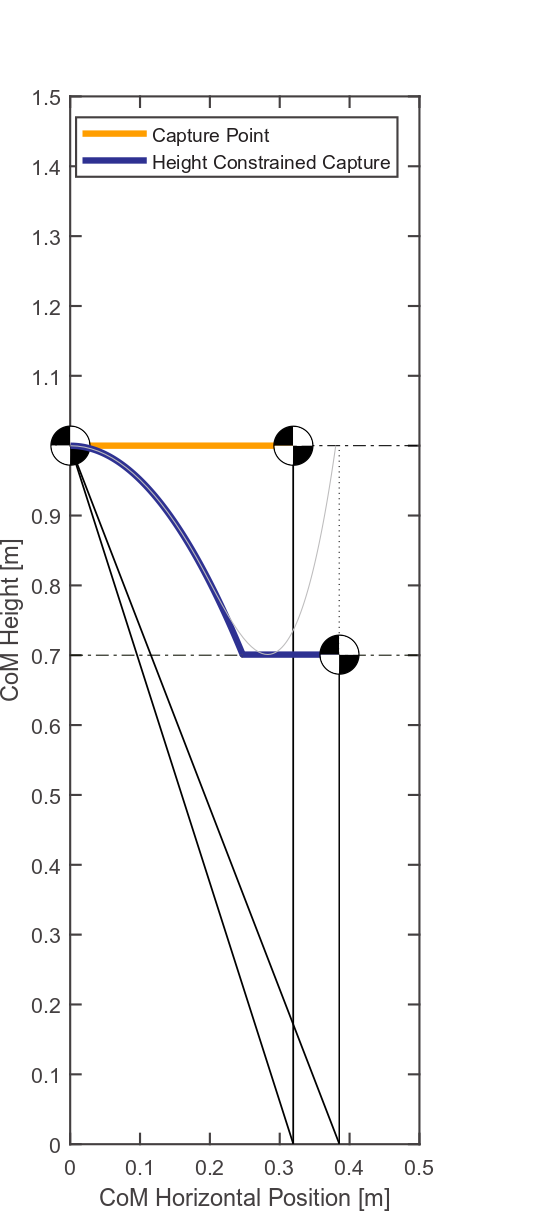
\includegraphics[width=.8\linewidth]{STYLESTUFF/CPvsMinHeight.png}
  \caption{}
   \label{fig:cpzmin}
  \end{subfigure}
  \begin{subfigure}{0.45\textwidth}
  \centering
  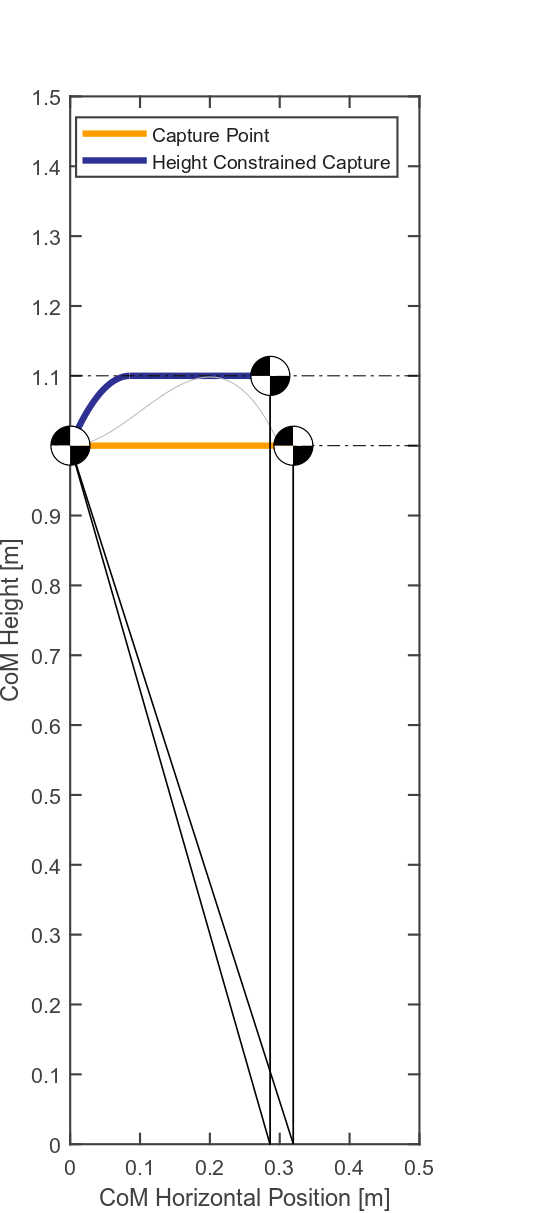
\includegraphics[width=.8\linewidth]{STYLESTUFF/CPvsHeight.png}
   \caption{}
    \label{fig:cpzmax}
  \end{subfigure}
  \caption{The height constrained capture limits for $\dot{x}_0=1.0$, $z_0=1.0$, (a) $z_{min}=0.7$ and (b) $z_{max}=1.1$. The grey plots are made with the method of \cite{koolen2016balance} and show that its final horizontal positions lie between the limit and the \ac{CP}. }
  \label{fig:cpz}
\end{figure}

%% Discussion
\section{Discussion}
In this chapter three different measures are proposed related to capturability of the point-mass, point-foot model, with an initial velocity that is horizontal. To summarize, these measures are:
\begin{itemize}
	\item A capture region or limit that only takes into account the unilaterality of contact constraint $\vect{f}_{leg}>0$.
	\item The closest possible capture location under a maximum height constraint $z_{max}$.
	\item The influence of an impact on the \ac{CP}.
\end{itemize}
These points or regions may not be of value for direct application, as they take a very limited amount of constraints into account on the model. However, just like with \ac{CP} and \ac{ICP}, they can be used for having an approximate guess of how the system dynamics will evolve over time. All of the proposed measures can be expressed in the systems current state and a maximum height constraint and are relatively computationally cheap compared to most optimization strategies, like trajectory optimization \cite{kelly2017introduction}.\\
The height constraint capture point might for example be used in an initial guess in an optimization algorithm, maybe factored down with a scaling value. The impact influence capture point can have value for motions where impacts at touch down can be expected beforehand, as for example in a planning or control strategy for robots that walk with straightened legs, as in \cite{griffin2018straight}. Moreover, as all three points are not dependent on any $y$-variable and can therefore be decoupled, they can be used without modification in \ac{3D} as well.
%
% Another appendix chapter
\chapter{Constrained Orbital Energy Trajectories}
[GEBRUIK LIMITS IN ALPHA EN LEG UIT OF GRADIENT NIET KAN] The inputs of height acceleration or inputs along the virtual leg have a changing effect proportional to the distance from the point foot. Next to this, if the goal of capture is considered, there exist a predetermined final point in the resulting trajectory of the control law. Namely, where the point-mass is above the point-foot, or the instable equilibrium of the inverted pendulum. With a simple proportial control law, no effects forward in time would be known. To have knowledge of the state variables of the model forward in time, the \ac{LIP} orbital energy, discussed in \ref{subsec:liporbit}, was extended by a height varying version by writing the height as a function of the horizontal position in  \cite{pratt2007derivation}, as mentioned in \ref{subsec:nonorbit}. This extra bit of information can be used in different ways, as for example in replanning the dynamic plan, or in \ac{MPC}. Depending on the way a dynamic plan is generated, the distinctionb between \ac{MPC} and dynamic replanning can be very small. In this chapter, the \ac{MPC} from \cite{koolen2016balance} is extended with constraints, which can be used for either dynamic replanning or \ac{MPC}.

%% Constraint matrix/polynomial
\section{Constraint Matrix}
In \cite{koolen2016balance}, the final horizontal velocity $\dot{x}_f$ is set to zero, as this leads to a capture trajectory. However, the trajectories are unconstrained and can become unrealistically high, as shown in \figref{fig:cpbal}. If from the final velocity is left open from the nonlinear orbital energy, this can be used in constrained optimization. A recap of Equation \ref{eq:eorbit}, but setting the final horizontal position zero:
\begin{equation}
    \frac{1}{2}\dot{x}^2\bar{f}^2(x)+gx^2f(x) - 3g\int_{0}^xf(\xi)\xi d\xi = \frac{1}{2}\dot{x}_0^2\bar{f}^2(0).
\end{equation}
Note that $\bar{f}^2(0)=(f(0)-f'(0)*0)^2=f(0)^2$. The additional nonzero term on the right side of the orbital energy equation can be added in the constraint matrix of \cite{koolen2016balance}. The 4x4 constraint matrix reads as:
\begin{equation}
    \underbrace{\begin{bmatrix}1 & 0 & 0 & 0 \\ 
     1 & x_0 & x_0^2 & x_0^3\\
     0 & 1 & 2x_0 & 3x_0^2\\
     \frac{3}{2}gx_0^2 & gx_0^3 & \frac{3}{4}gx_0^4 & \frac{3}{5}gx_0^5\\
     \end{bmatrix}}_{\matr{A}}
     \underbrace{\begin{bmatrix}
     c_0\\
     c_1\\
     c_2\\
     c_3\\
     \end{bmatrix}}_{\vect{c}}=
     \underbrace{\begin{bmatrix}
     z_f\\
     z_0\\
     \frac{\dot{z}_0}{\dot{x}_0}\\
     k\\
     \end{bmatrix}}_{\vect{b}}.
\end{equation}
Recap that the function $f(x)$ is constrained to be a cubic polynomial: $f(x)=\sum_{i=0}^3 c_ix^i$. The last constraint in the matrix is the constraint on conservation of orbital energy. Note that the integal term in the orbital energy equation read as: $3g\int_{0}^xf(\xi)\xi d\xi = 3g\sum_{i=0}^3\frac{1}{i+2}c_ix_0^{i+2}$. The last constraint of the matrix reads after addition of the final velocity term as:
\begin{equation}
		3g\int_{0}^xf(\xi)\xi d\xi =\frac{1}{2}\dot{x}^2\bar{f}^2(x)+gx^2f(x) - \frac{1}{2}\dot{x}_0^2\bar{f}^2(0),
\end{equation}
and in terms of the cubic polynomial as:
\begin{align}
	3g\sum_{i=0}^3\frac{1}{i+2}c_ix_0^{i+2}& = \frac{1}{2}(\dot{x}_0z_0-\dot{x}_0x_0)^2 + gx_0^2z_0 - \frac{1}{2}z_f^2\dot{x}_f^2,\\
	&=k,
\end{align}
where $k$ is the last value in vector $\vect{b}$. Using the polynomial description and having a nonzero final velocity $\dot{x}_f$, the final height $z_f$ constraint results in a final height velocity $\dot{z}_f$ equal to the gradient:
\begin{align}
 	f'(0) &= \frac{\dot{z}_f}{\dot{x}_f},\\
 	\dot{z}_f &= f'(0)\dot{x}_f.
\end{align}
If a nonzero final velocity $\dot{x}_f$ is considered, the pendulum is at the point $x=0$ at a point during swing. It could be desirable later, to have zero height velocity $\dot{z}_f$ at this point. The first constraint $f(0)=z_f$ in the matrix can be replaced by this constraint on this final gradient:
\begin{equation}
    \underbrace{\begin{bmatrix}0 & 1 & 0 & 0 \\ 
     1 & x_0 & x_0^2 & x_0^3\\
     0 & 1 & 2x_0 & 3x_0^2\\
     \frac{3}{2}gx_0^2 & gx_0^3 & \frac{3}{4}gx_0^4 & \frac{3}{5}gx_0^5\\
     \end{bmatrix}}_{\matr{A}}
     \underbrace{\begin{bmatrix}
     c_0\\
     c_1\\
     c_2\\
     c_3\\
     \end{bmatrix}}_{\vect{c}}=
     \underbrace{\begin{bmatrix}
    \frac{\dot{z}_f}{\dot{x}_f}\\
     z_0\\
     \frac{\dot{z}_0}{\dot{x}_0}\\
     k\\
     \end{bmatrix}}_{\vect{b}}
\end{equation}
Note that the matrix is still full rank, as long as $x_f$ and $\dot{x}_f$ are nonzero.
%\begin{equation}
%    u = \frac{g + f''(x)\dot{x}^2}{\bar{f}(x)}
%\end{equation}

% Height Constraint
\subsection{Height Constraint}
Using the previous problem with an undetermined final velocity $\dot{x}_f$, a height constraint can be used in optimization. Algorithm \ref{alg:h} shows how the polynomial values can be found under this constraint. The maximum height of trajectory being optimized over is at location $x_{zmax}$, which has two solutions. In \figref{fig:polheight} two resulting polynomials are shown from Algorithm \ref{alg:h}, one with the final height constraint and one for the constraint on the final gradient. Notice that the peak for the maximum value in both plots lies on the maximum $x$-value from the solutions of the locations where the gradient as zero. Therefore, in Algorithm \ref{alg:h} the solution that corresponds to this peak is sufficient, if a constraint on the maximum value is considered. In the plot of the figure, the entire polynomial is shown for explanatory reasons, but in control or planning only the part would be used from the starting point $x=-0.25$.
\begin{equation}
	\dot{x}_{f,cp} = \sqrt{\dot{x}_0^2-\frac{g}{z}x^2}
\end{equation}
\begin{equation}
	\dot{x}_{f,cp,maxheight} = \sqrt{\dot{x}_{0,I}^2-\frac{g}{z}(x+\frac{\dot{z}_I}{g}\dot{x}_{0,I})^2}
\end{equation}
\begin{equation}
	\alpha =\frac{\dot{x}_{f,cp} -\dot{x}_{f,cp,maxheight}}{N}
\end{equation}
$N=30$.

\begin{algorithm}
\caption{Find cubic polynomial constants under height constraint}
\label{alg:h}
\begin{algorithmic}[1]
    \State $\dot{x}_{f}\gets 0$\Comment{Initial guess}
        \Repeat
            \State $\vect{c}\gets \matr{A}^{-1}\vect{b}(\dot{x}_{f})$ \Comment{Find polynomial constants}
            \State $x_{zmax}\gets \frac{-2c_2 - \sqrt{4c_2^2-12c_3c_1}}{6c_3}$ \Comment{Traj. peak lies on highest x}
            \State $z_{max} \gets c_0 + c_1x_{zmax} + c_2x_{zmax}^2+ c_3x_{zmax}^3$ \Comment{Corresponding height}
            \State $\dot{x}_{f} \gets \dot{x}_{f}+\alpha$   \Comment{Some smart increment}
        \Until{$z_{max}<z_{const}$}\\
    \Return $\vect{c}$
\end{algorithmic}
\end{algorithm}
\begin{figure}[h]
\centering
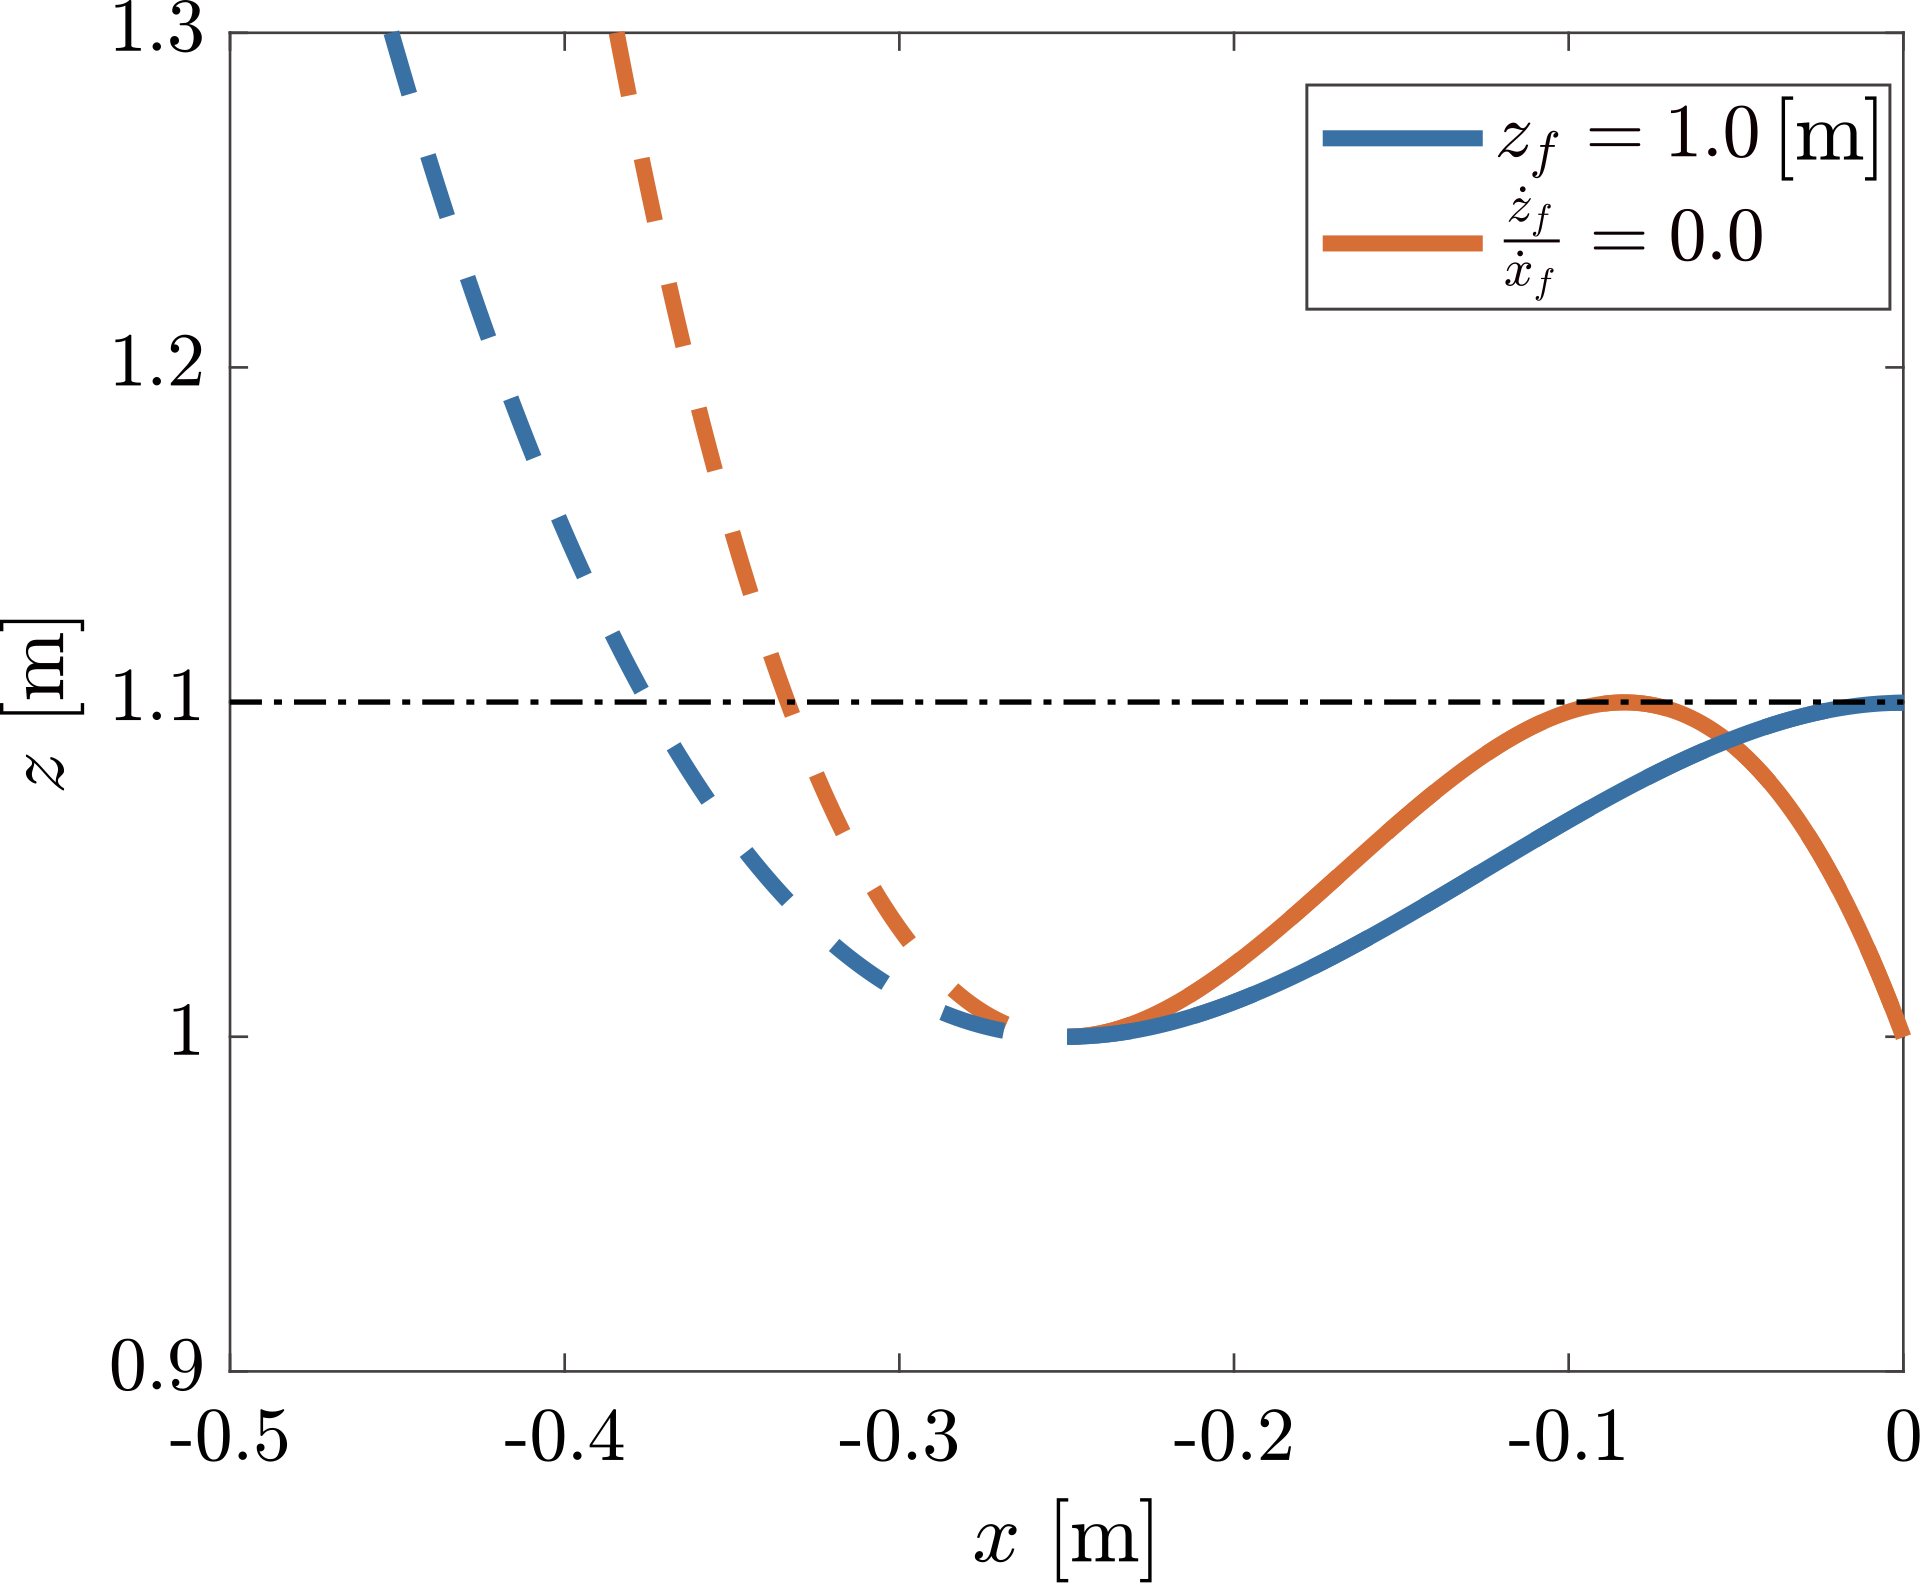
\includegraphics[width=0.6\textwidth]{STYLESTUFF/polynomialHeightViz.png}
\caption{Resulting polynomials as output from Algorithm \ref{alg:h} with two different constraints on the final value. Initial conditions are $x_0=-0.25$, $\dot{x}_0=1.0$, $z_0=1.0$ and $\dot{z}_0=0$. Blue plot: $\dot{x}_f=0.552$, red plot: $\dot{x}_f=0.576$, $z_{max}=1.1$. }
\label{fig:polheight}
\end{figure}


% leg length constraint
\subsection{Leg Length Constraint}
For application, a leg e length constraint would be more realistic than a height constraint. The leg length as a function of $x$ can be expressed using the Pythagorean theorem:
\begin{equation}
	l^2(x) = f(x)^2 + x^2,
\end{equation}
where $l$ the length of the virtual leg. The solution to $f(x)^2$ is:
\begin{equation}
f(x)^2=(\sum_{n=0}^3 c_n x^n)^2 = \sum_{n=0}^3 c_n^2 x^{2n} + 2\sum_{\substack{n=1 \\ i+j=n \\ i < j}}^5 c_i c_j x^n. 
\end{equation}
However, as the gradient needs to be computed to obtain the locations of the peaks in the polynomial, $f(x)^2$ is approximated with:
\begin{equation*}
	f(x)^2\approx \sum_{n=0}^3 c_n^2 x^{2n}.
\end{equation*}
With this formulation of the squared function, the squared $x$ position of maximum leg length is computed in the following way:
\begin{align}
	\frac{d(f(x)^2+x^2)}{dx}&=0\\
	\frac{d(f(x)^2+x^2)x}{dx}&=0\\
	6c_3^2 x^4 + 4 c_2^2 x^2 + 2+2c_1^2 &= 0\\
	6c_3^2 (x^2)^2 + 4 c_2^2 (x^2) + 2+2c_1^2 &= 0
\end{align}
Again, the value of the maximum peak lies on the highest $x$ value of the two locations where the gradient is zero. Algorithm \ref{alg:ll} shows how the polynomial constants can be found under the leg length constraint. In Figure \ref{fig:pollength}, it can be seen that the resulting polynomials do not violate the maximum length constraint.
\begin{algorithm}
\caption{Find cubic polynomial constants under leg length constraint}
\label{alg:ll}
\begin{algorithmic}[1]
    \State $\dot{x}_{f}\gets 0$\Comment{Initial guess}
        \Repeat
            \State $\vect{c}\gets \matr{A}^{-1}\vect{b}(\dot{x}_{f})$ \Comment{Find polynomial constants}
            \State $x_{lmax}^2 \gets \frac{-4c_2^2+\sqrt{16c_2^4-24c_3^2(2+2c_1^2)}}{12c_3^2}$ \Comment{$d(f(x)^2+x^2)/dx=0$}  
            \State $x_{lmax}\gets-|\sqrt{x_{l^2max}}|$                \Comment{Complex solutions}
            \State $l_{max}^2 \gets x_{lmax}^2 + (c_0 + c_1x_{zmax} + c_2x_{zmax}^2+ c_3x_{zmax}^3)^2$ 
            \State $\dot{x}_{f} \gets \dot{x}_{f}+\alpha$   \Comment{Some smart increment}
        \Until{$l_{max}^2<l_{const}^2$}\\
    \Return $\vect{c}$    
\end{algorithmic}
\end{algorithm}
\begin{figure}[h]
\centering
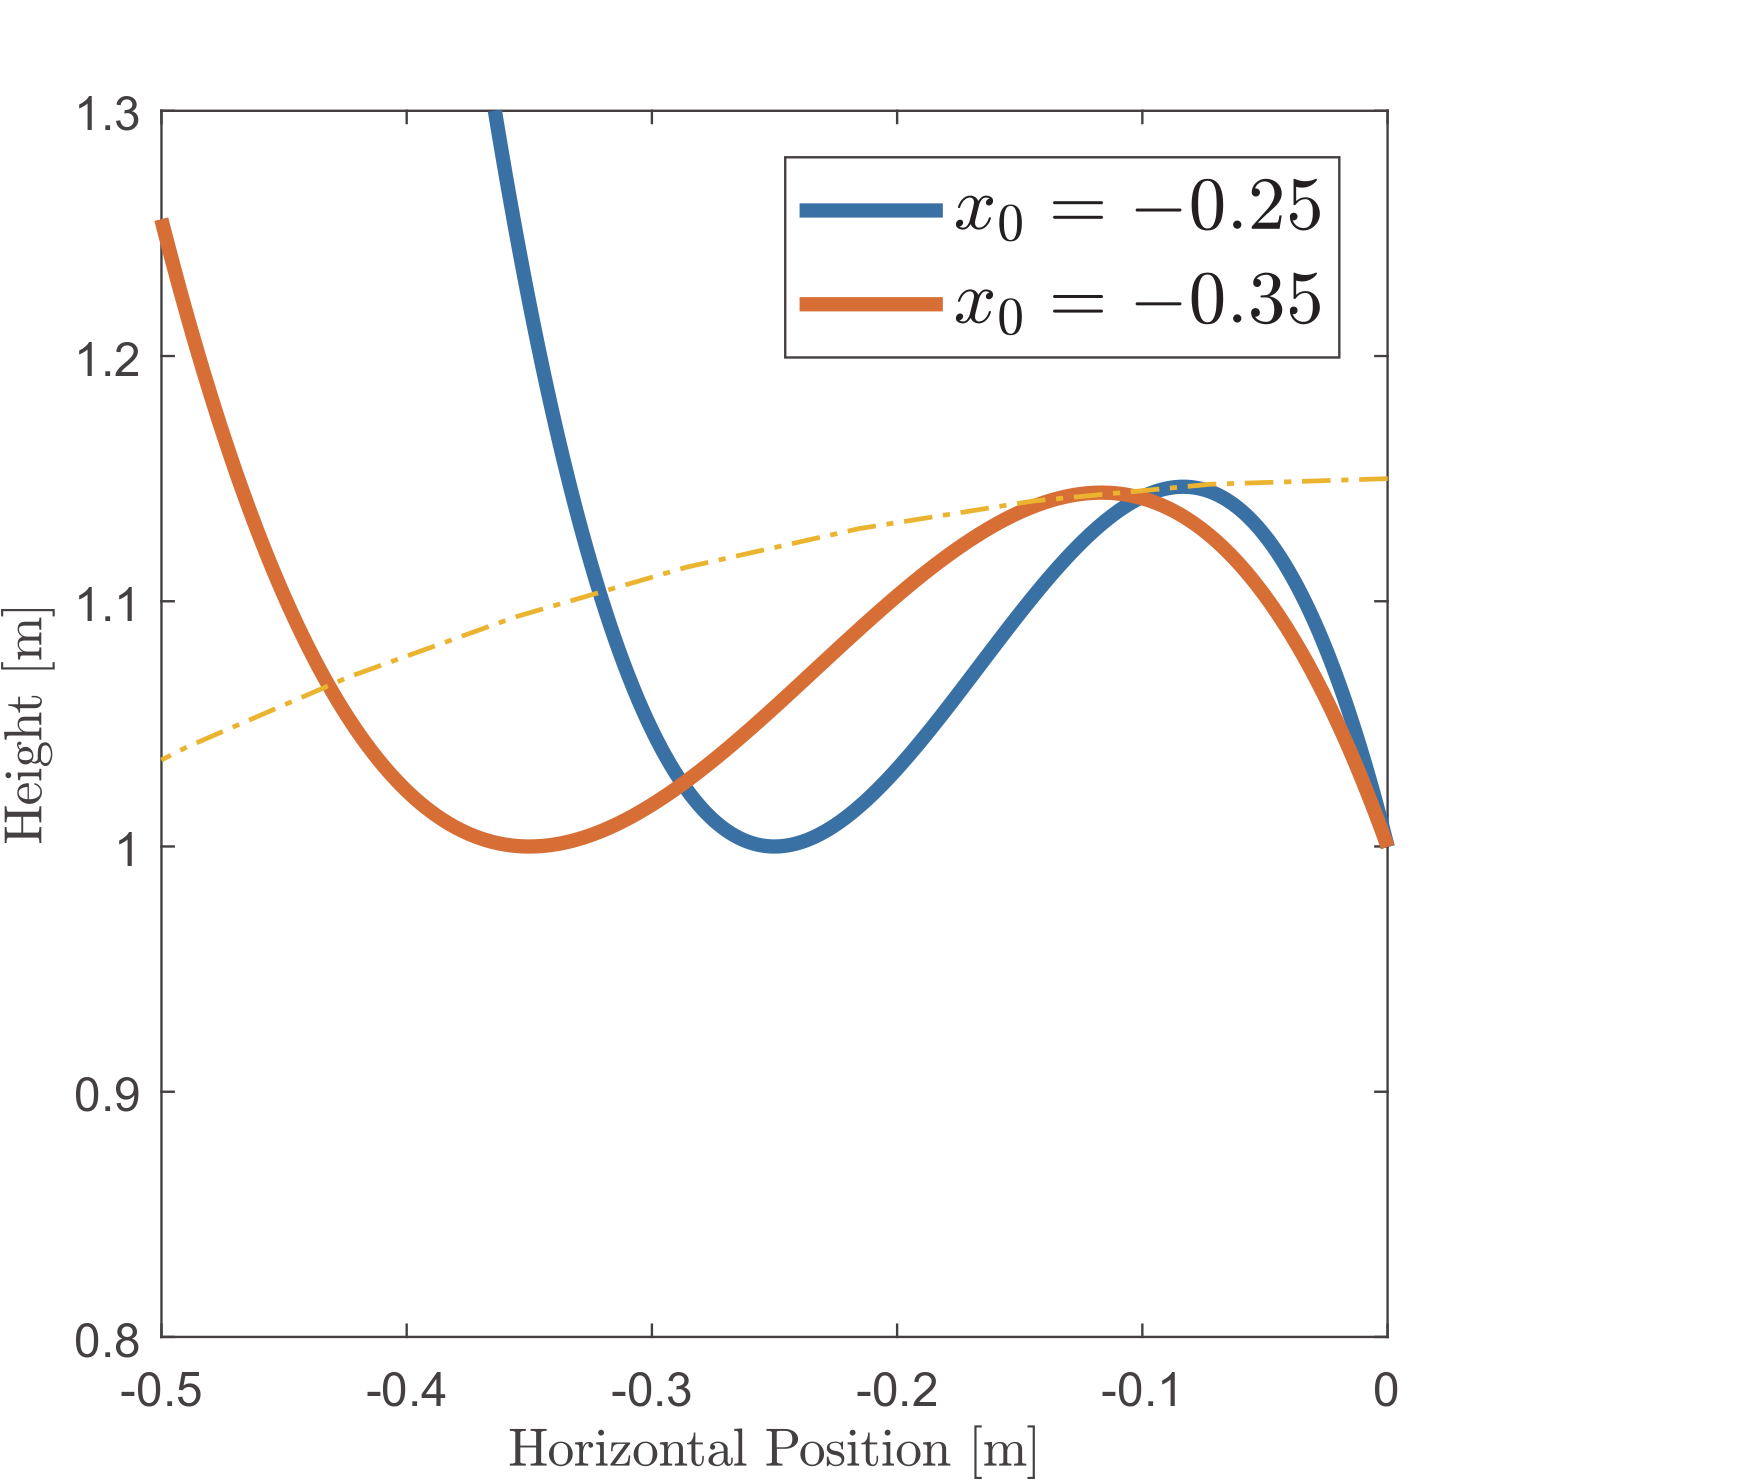
\includegraphics[width=0.6\textwidth]{STYLESTUFF/polynomialLengthViz.png}
\caption{Resulting polynomials as output from Algorithm \ref{alg:ll} with two different initial values under the final height constraint $z_f=1.0$. Other initial conditions are $\dot{x}_0=1.4$, $z_0=1.0$ and $\dot{z}_0=0$. Blue plot: $\dot{x}_f=1.107$, red plot: $\dot{x}_f=0.724$, $l_{max}=1.15$. }
\label{fig:pollength}
\end{figure}
% discussion
\section{Discussion}
The proposed algorithms can find a trajectory that gives knowledge of the estimated system state of a \ac{2D} point-foot, point-mass model until the $x$-coordinate of the point-foot. To the method of \cite{koolen2016balance}, a constraint is added on the maximum height, a maximum leg length constraint and the possibility is proposed to exchange the final height constraint with a final gradient constraint. Remarkable is that the final gradient constraint gives a higher final velocity $\dot{x}_f$ compared to the default height constraint in \figref{fig:polheight}. This is caused by the polynomial shapes, as the blue plot, under constraint $z_f$, has a steeper gradient in the first part of the trajectory after $x_0$. This is the crucial part in the trajectory for a acceleration or deceleration action in $x$-direction, as can be seen in for example Equation \eqref{eq:dynamicsprattstyle}. \\
One of the algorithms can be used in \ac{MPC}, however, it lacks a lot of properties important for application on humanoid robot as Atlas for example:
\begin{itemize}
	\item The method is only suited for a \ac{2D} control strategy.
	\item The resulting trajectory is limited by the shape of a cubic polynomial.
	\item The model is point-mass, point-foot and does not take the control options of feet or a body into account.
	\item The method is analytic and does not calculate for the next controller tick.
	\item Only a maximum height constraint is considered.
\end{itemize}

%
% Another appendix chapter
\chapter{Toward Application: Walking}\label{chap:walking}
The control strategy for a static, standing case presented in the previous chapter is two-dimensional. If the robot is walking, the horizontal \ac{CoM} position can lie outside the support polygon. The result of this is that the desired \ac{CoP} cannot always be placed in line with the \ac{ICP} error.  In this chapter, the bang-bang control law of Chapter \ref{chap:standing} is extended for the use in \ac{3D}.
% Experimental Setup
\section{Experimental Setup}
With the same motivation as in the previous chapter of applying a maximum acceleration possible in a worst-case scenario, a bang-bang control law can be used. In this section, to determine \textit{when} to turn the bang-bang controller on in \ac{3D},  tests are conducted preliminary to developing a controller. 

In the tests, a push is applied in the beginning of the \ac{SS} while the robot is walking. The stepping parameters used for the test situation are given in Table \ref{tab:stepping}, which are the default stepping parameters during testing in simulation. In \figref{fig:valwalkingtest}, the test setup in simulation is shown. The limited foothold options display that footstep location adjustment is not available as a balance strategy. In \figref{fig:3foot}, the \ac{ICP} and \ac{CMP} reference trajectory and the measured \ac{CoM} trajectory, without application of a push are made visible. 
\begin{table}[ht]
\caption{Stepping Parameters} % title of Table
\centering % used for centering table
\begin{tabular}{c c c } % centered columns (4 columns)
\hline\hline %inserts double horizontal lines
Parameter & Value & Unit \\
%heading
\hline % inserts single horizontal line
Step Legth & 0.5 &  [m]\\
Step Width & 0.25 & [m]\\
\acs{SS} Time & 0.6 & [s]\\
\acs{DS} Time & 0.15 & [s]\\
%[1ex] % [1ex] adds vertical space
\hline %inserts single line
\end{tabular}
\label{tab:stepping} % is used to refer this table in the text
\end{table}
\begin{figure}[h]
\centering
  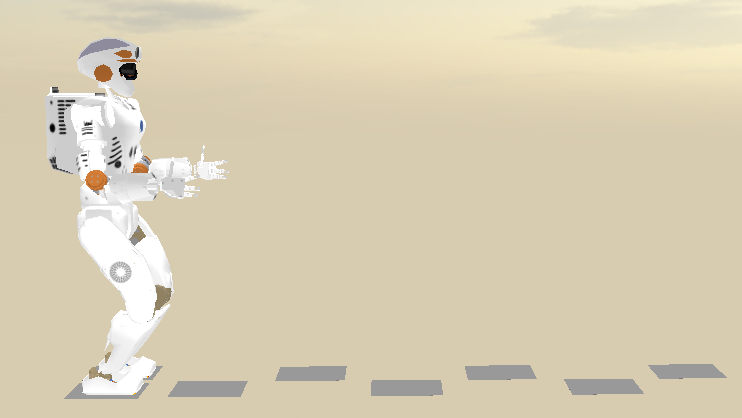
\includegraphics[width=.8\linewidth]{STYLESTUFF/valwalkingtest.png}
   \caption{Test setup for push recovery during walking in simulation. The limited foothold options show that footstep adjustment is not available as a balance strategy.}
    \label{fig:valwalkingtest}
\end{figure}
\begin{figure}[h]
\centering
  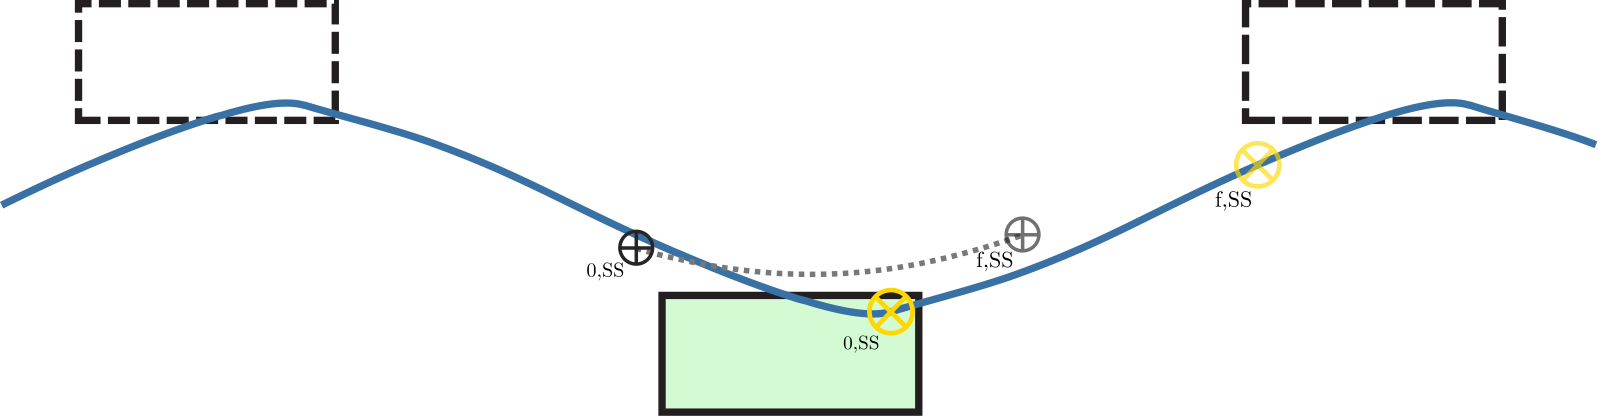
\includegraphics[width=.8\linewidth]{STYLESTUFF/ICPplan3StepComICPrSS.png}
   \caption{Trajectories during \ac{SS} in the horizontal plane (gray dotted lines). The gray area is the current footstep position.}
    \label{fig:3foot}
\end{figure}
%Preliminary observations

The following properties are observed, when applying pushes in different direction in the start of \ac{SS}:
\begin{enumerate}
	\item The direction of the \ac{ICP} error stays often approximately the same until transition to \ac{DS}.
	\item If the \ac{ICP} error is directed in the sagittal plane, the desired \ac{CMP} often remains somewhat in the same location.
	\item If the \ac{ICP} error is directed  in the coronal plane, the desired \ac{CMP} slides from back to the forth of the foot.
	\item The configuration and velocity near transition to \ac{DS} affects the robots ability to put its swing leg down at the desired time. 
\end{enumerate}
These properties are used as assumptions in the development of a control law.
% Methods
\section{Method}

\subsection{Avoiding Generating Additional Angular Momentum Rate}
First, the control law of the previous chapter is made suitable for $\rcmpd$ locations outside the support polygon. The motivation in the development of a control law is to request as less as possible additional angular momentum rate compared to the default setup, when using \ac{CoM} height variations for balance control. Therefore, the vertical motion controller generates and added desired momentum rate on top of the default controller. Under the assumption that the difference in $\rcopd$ and $\rcmpd$ is directly related to the resulting torque about the \ac{CoM}, the following is derived:
\begin{align}
    \dotldxy &= \frac{\cxy-\rcmpd}{z_0}(mg+\dotldz),\\
&=\frac{\mathbf{c}_{xy}-(\rcopd+\frac{\taucom}{(mg+\dotldz})}{z}(mg+\dotldz), \\
&=\frac{\mathbf{c}_{xy}-\rcopd}{z}(mg + \dotldz)- \frac{\taucom}{z},
\end{align}
If the location of $\rcmpd$ is outside the polygon, the vertical motion controller uses $\rcopd$ for additional height variation. The computation reads as follows:
 \begin{align}
\dot{\mathbf{l}}_{xy,d}&=\frac{\mathbf{c}_{xy}-\rcopd}{z}(mg+\dotldz) - \frac{\taucom}{z},\\
&=\underbrace{ \frac{\mathbf{c}_{xy}-\mathbf{r}_{cmp,d}} {z_0}mg}_{\dotldxylip}  + \underbrace{\frac{\mathbf{c}_{xy}-\mathbf{r}_{cop,d}}{z}\dotldz}_{\dotldxyheight},
\end{align}
where $\dotldxyheight$ is the additional desired horizontal linear momentum rate from the vertical motion controller and $\dotldxylip$ the momentum rate from the default control law.

In Figure \ref{fig:rcopdvsrcmpd}, it is visually explained in \ac{2D} how this computation of $\dotldxy$ does not require additional angular momentum from the robot. However, the resulting \ac{CMP} location would be different.

\begin{figure}
\centering
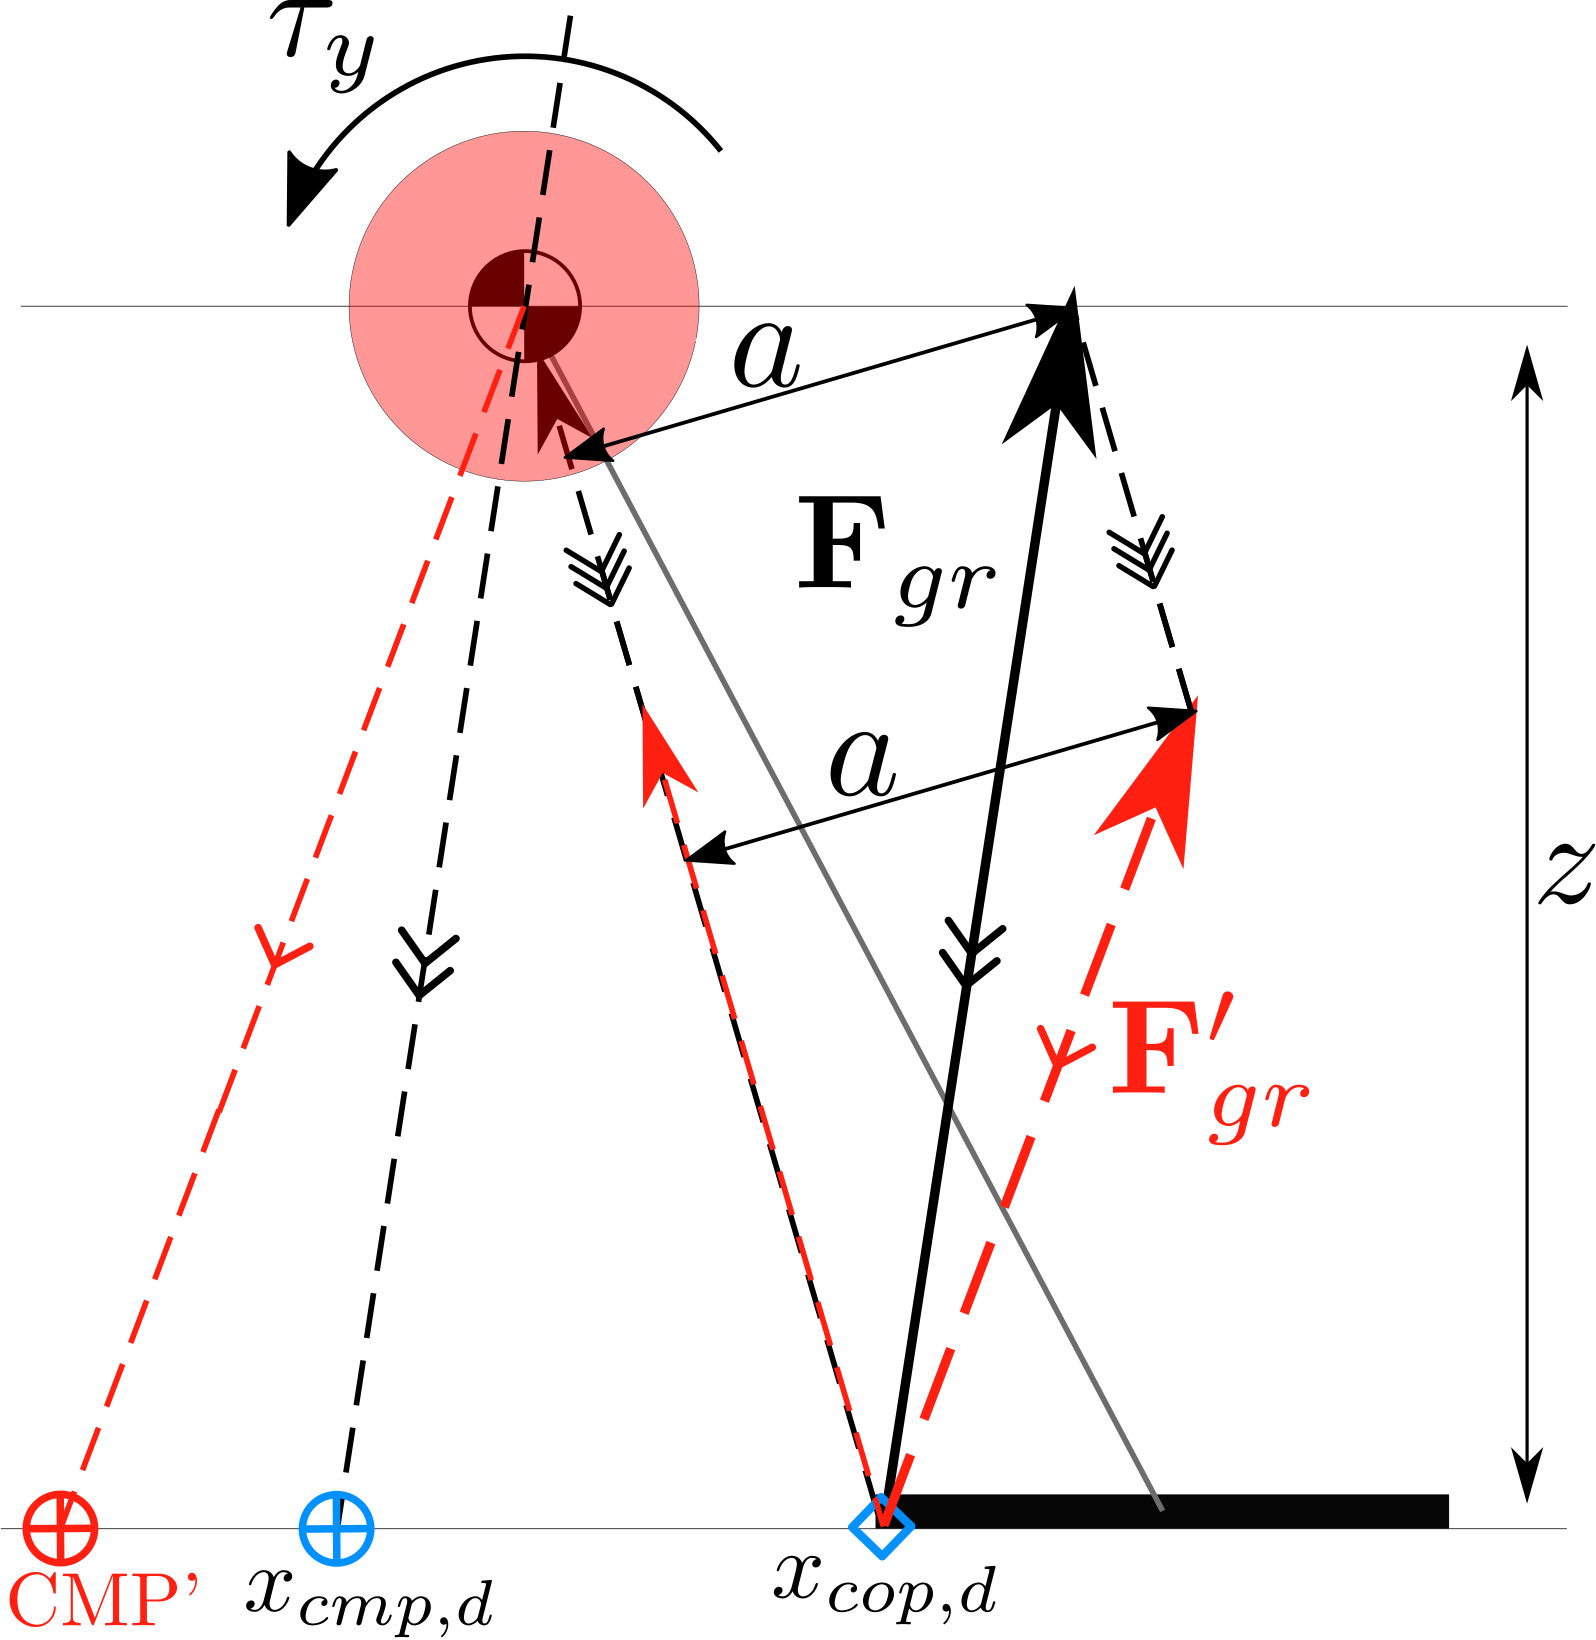
\includegraphics[width=0.45\textwidth]{STYLESTUFF/2DControlStrategyViz.png}
\caption{Requesting additional horizontal momentum rate based on $\rcopd$ will not need additional angular momentum to be achievable, as the scalar offset $a$ is equal. However, the resulting \ac{CMP} will be in a different location than $\rcmpd$.}
\label{fig:rcopdvsrcmpd}
\end{figure}
\subsection{Alignment Angle and Relative Distance}
If the \ac{CoM} is outside the support polygon, the local virtual leg between $\rcopd$ and the horizontal \ac{CoM} location $\cxy$ may not be aligned with direction of the \ac{ICP} error $\icpe$. This results in the leg applying force in a different direction than is needed to cancel the error, which can result in additional error in another direction. Also, if $\cxy$ is close to the polygon edge, the distance with $\rcopd$ might be very small, such that height changes have little to potentially no effect. To take these two aspects into account, the following variables are introduced, which help to determine when to use \ac{CoM} height variation for balance:
\begin{itemize}
	\item $\phi$: the alignment angle between the virtual leg between $\rcopd$ and $\cxy$ and the \ac{ICP} error $\icpe$;
	\item $\delta$: the effective distance between $\rcopd$ and $\cxy$. The is the distance between the two points in the direction of the \ac{ICP} error $\icpe$.
\end{itemize}

In \figref{fig:phiViz}, the two variables are graphically explained using the stance foot position of \figref{fig:3foot}. $\rcmpd$ is allowed to move a small distance outside the polygon. In \figref{fig:phiVizc}, the angle $\phi$ is zero and $\delta$ is relatively large. This is a relatively suitable error for height control. In \figref{fig:phiVizd}, the angle $\phi$ is $90$ degrees and therefore the distance $\delta$ is zero. In this configuration, \ac{CoM} height variation would not help driving the error back. Furthermore, an additional error would occur orthogonal to the current $\icpe$.
\begin{figure}[h]
\centering
  \begin{subfigure}{0.49\textwidth}
    \centering
  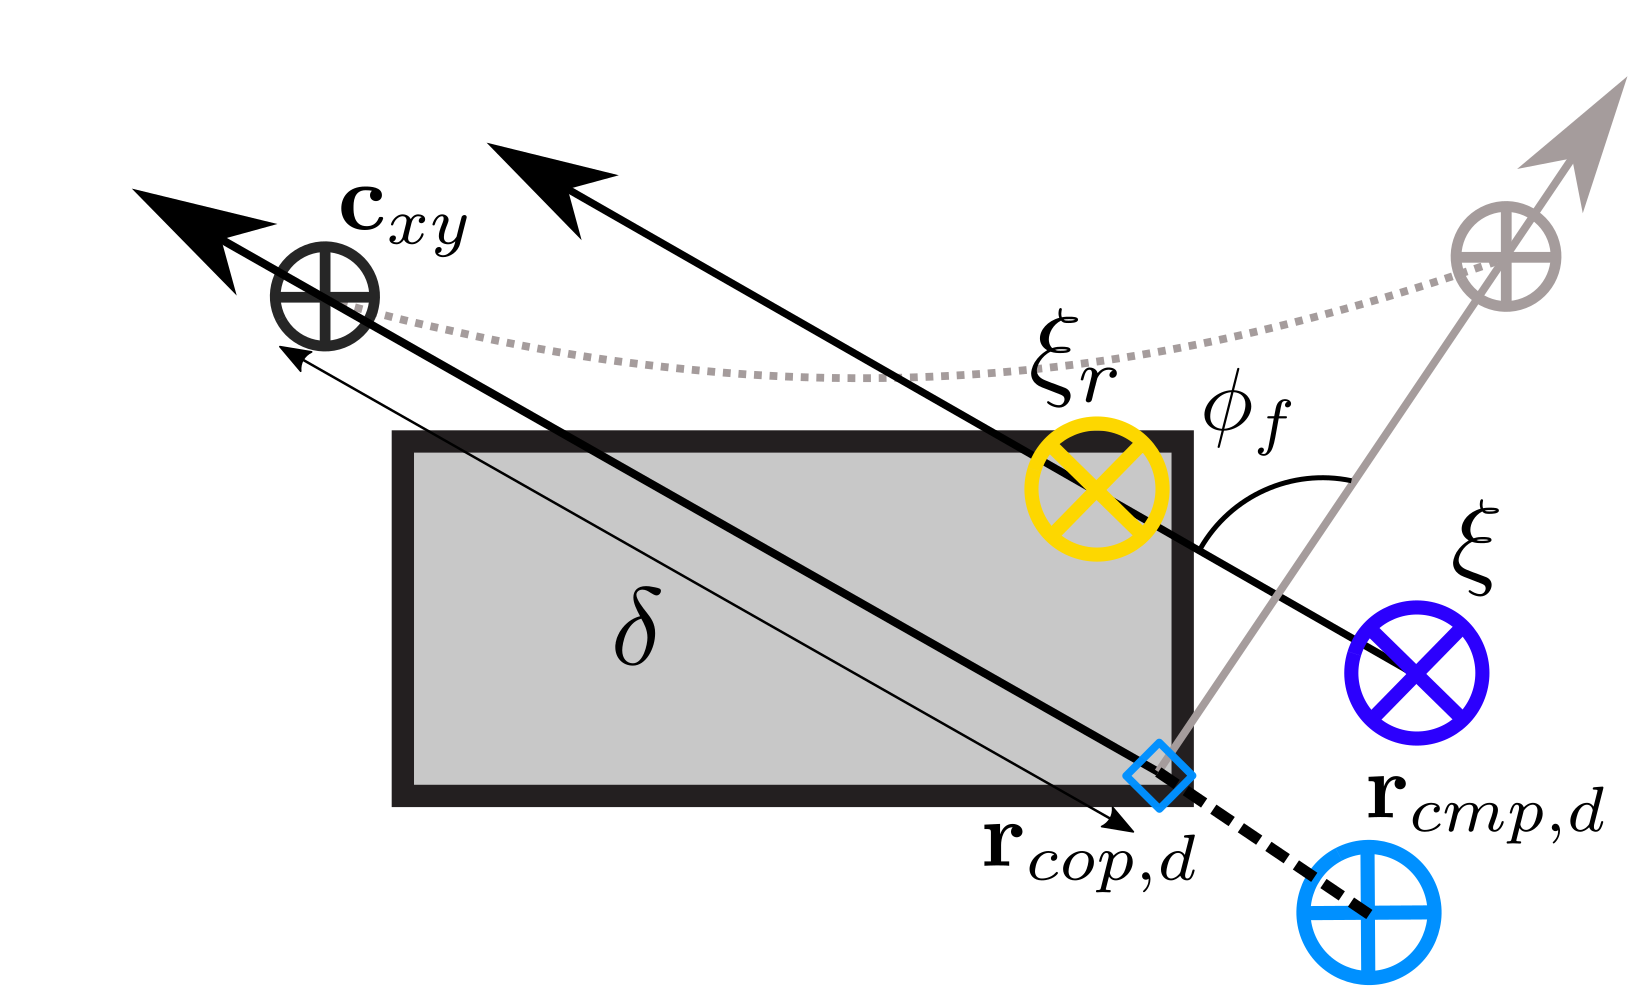
\includegraphics[width=.7\linewidth]{STYLESTUFF/ICPplanStartSSPhiViz0.png}
    \caption{}
     \label{fig:phiVizc}
  \end{subfigure}
  \begin{subfigure}{0.49\textwidth}
    \centering
  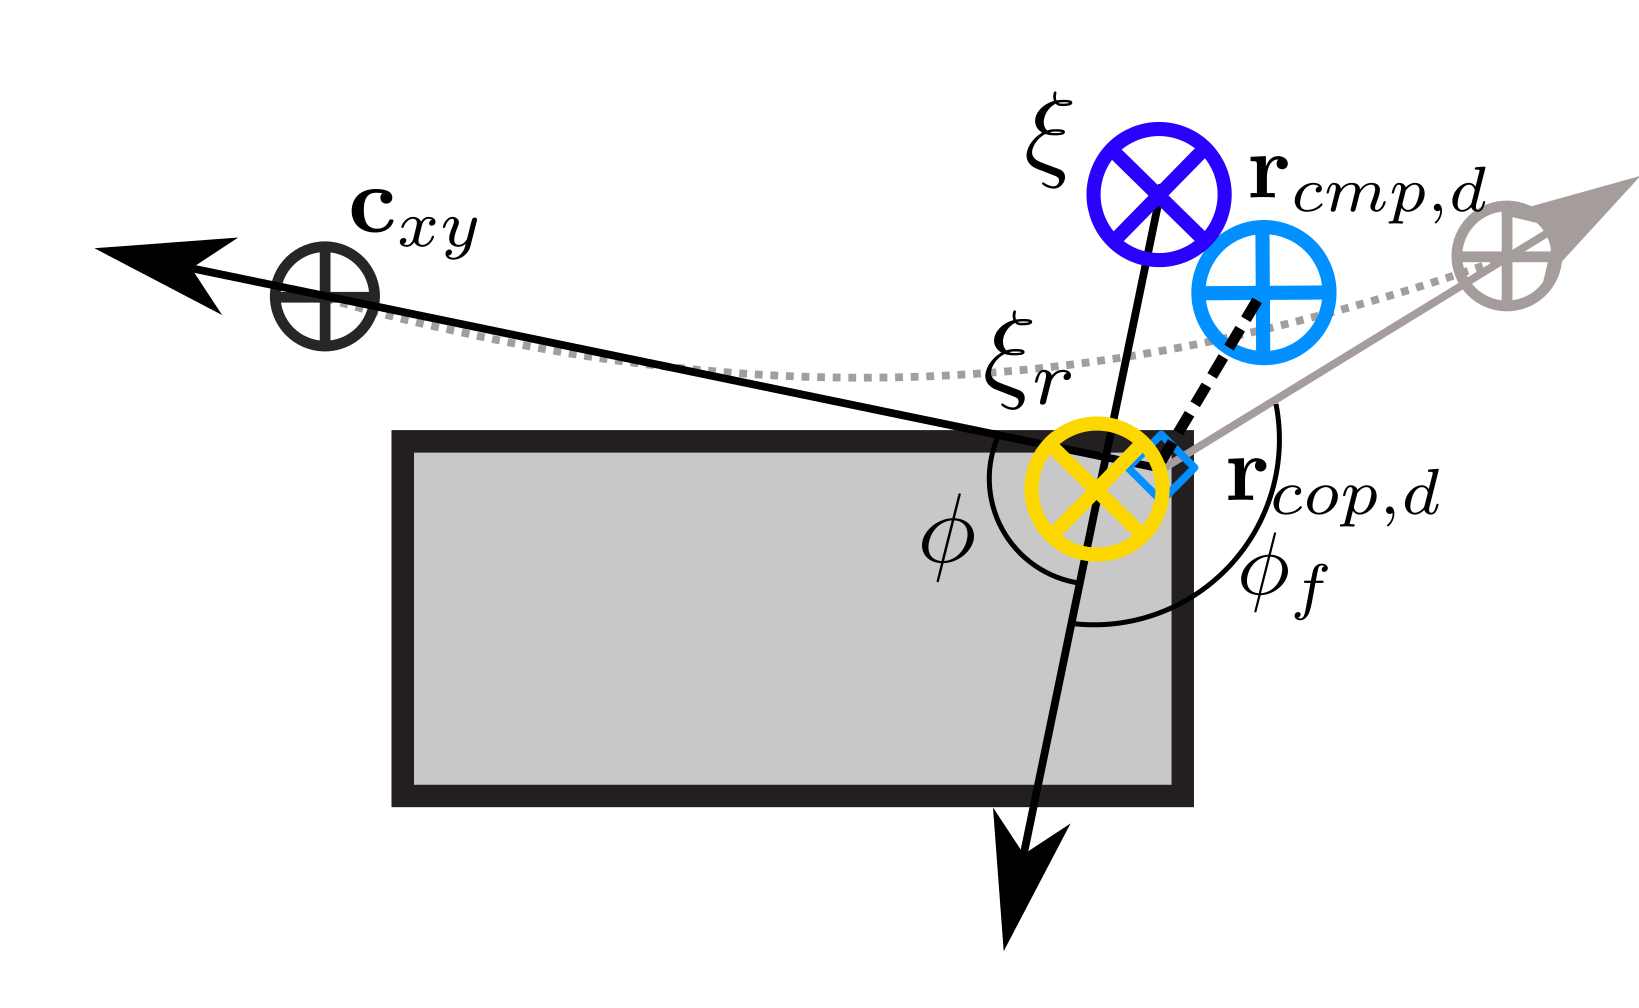
\includegraphics[width=.7\linewidth]{STYLESTUFF/ICPplanStartSSPhiViz90.png}
    \caption{}
     \label{fig:phiVizd}
  \end{subfigure}
  \caption{Vizualizations of $\phi$ and $\delta$ for the configuration at start of \ac{SS}.}
  \label{fig:phiViz}
\end{figure}

\subsection{Actions}
The alignment angle $\phi$ and the relative distance $\delta$ are used to select a control action, if the $\rcmpd$ crosses the polygon edge. From the assumptions of the preliminary observations $1$ and $2$, it is assumed that the angle $\phi$ will be dependent on the current $\icpe$ and $\rcopd$ throughout \ac{SS} if $\icpe$ is directed in the sagittal plane. Therefore, the additional variables $\delta_f$ and $\phi_f$ are used, which are the expected alignment and distance in the end of \ac{SS}, based on the \ac{CoM} location coming from the \ac{ICP} planner. Also, from assumption $3$, $\phi$ is not used if a push is in the coronal plane. Throughout \ac{SS}, the whole foot length is available for future $\rcmpd$ placements that could correct any additional error. Based on the discussed variables, the following three actions can be selected:
\begin{itemize}
	\item \textbf{Positive alignment}: At the current control tick, $\phi$ is relatively misaligned and $\delta$ relatively large for a push in the sagittal plane, or $\delta$ is relatively large for a push in the coronal plane. Also, $\phi$ has to be smaller than $\frac{1}{2}\pi$ [rad], as the virtual leg must be in direction of the \ac{ICP} error to make additional force effective. A bang-bang action is activated that starts with a positive `bang'.
	\item \textbf{Prepare}: At the current control tick, $\phi$ is relatively misaligned or $\delta$ is relatively small, but $\phi_f$ and $\delta_f$ are at values suitable for the positive alignment phase. The \ac{CoM} height is gradually lowered to the minimum height, after which the `bang-bang' action of the positive alignment phase is activated.
	\item \textbf{Default}: All decisions variables $\phi$, $\delta$, $\phi_f$ and $\delta_f$ are at such values, that vertical \ac{CoM} motion does not improve recovery. The default height control law is used and no additional height changes are considered.
\end{itemize}

In \figref{fig:phi}, four cases are shown for different actions. In \figref{fig:phiViza} and , a positive alignment action is introduced, as $\phi$ is relatively small and $\delta$ relatively large. In \figref{fig:phiViza}, the prepare action is used, as $\delta_f$ and $\phi_f$ are more suitable for height control. In \figref{fig:phiVize}, the positive alignment action is used, as the current $\delta$ is relatively large. In \figref{fig:phiVizf}, the default action is activated, as $\delta$ is small throughout \ac{SS}.
\begin{figure}[h]
\centering
  \begin{subfigure}{0.49\textwidth}
  \centering
  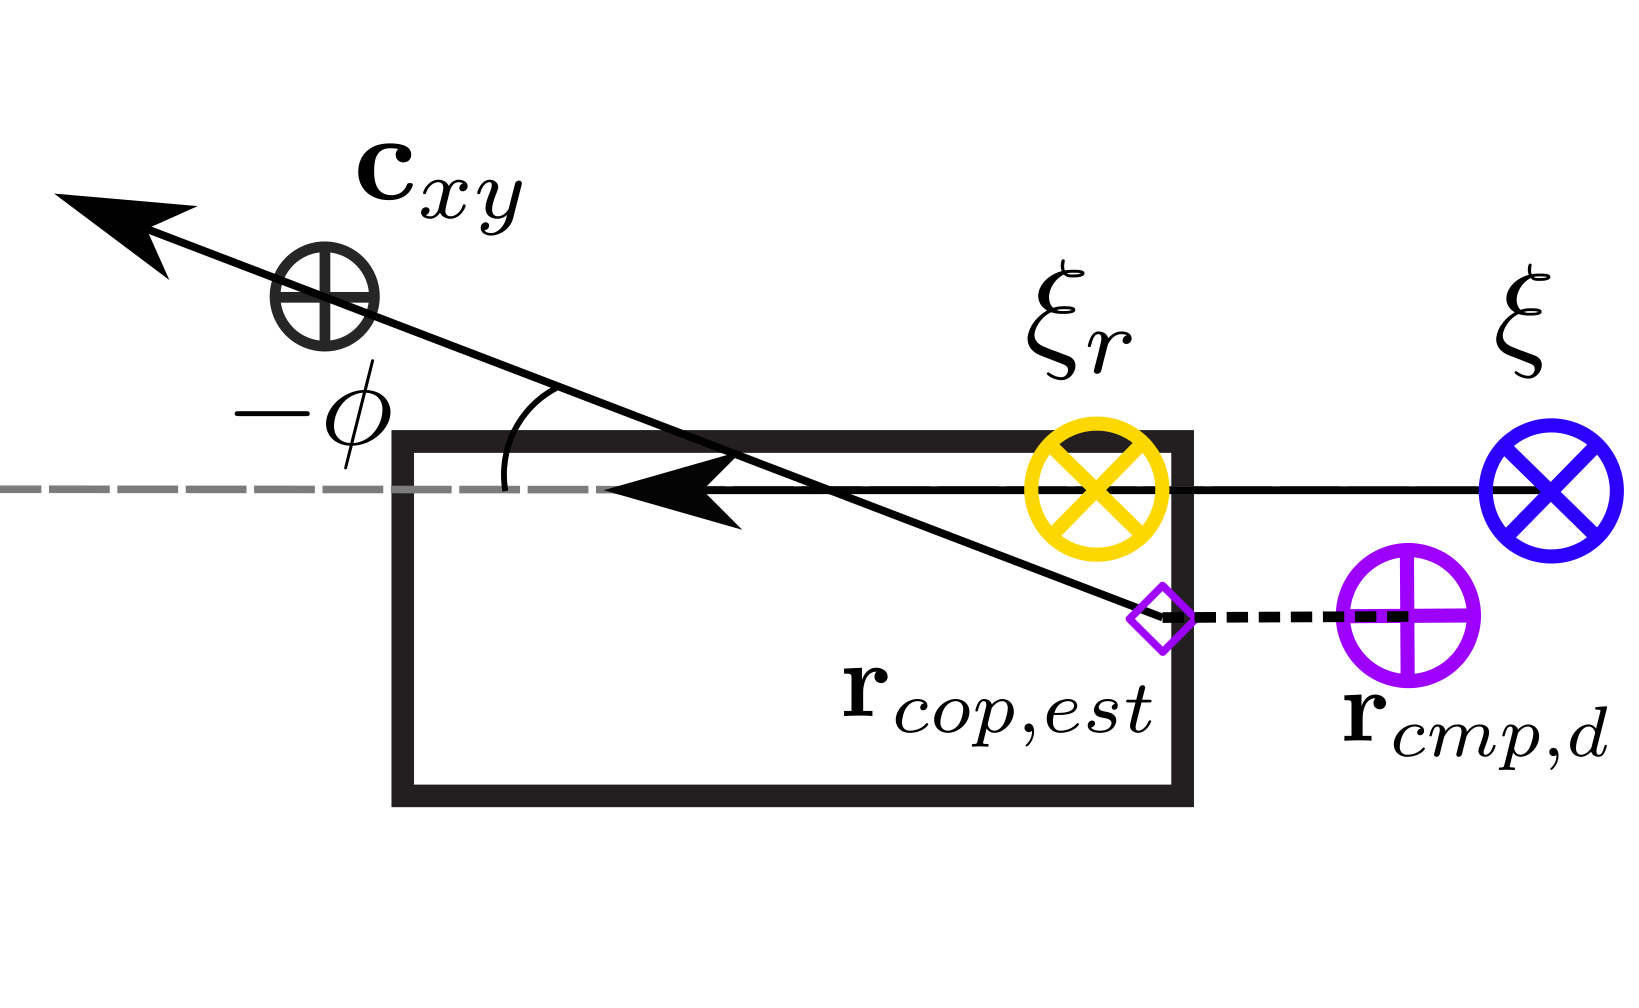
\includegraphics[width=.7\linewidth]{STYLESTUFF/ICPplanStartSSPhiVizNegError.png}
   \caption{}
    \label{fig:phiViza}
  \end{subfigure}
  \begin{subfigure}{0.49\textwidth}
    \centering
  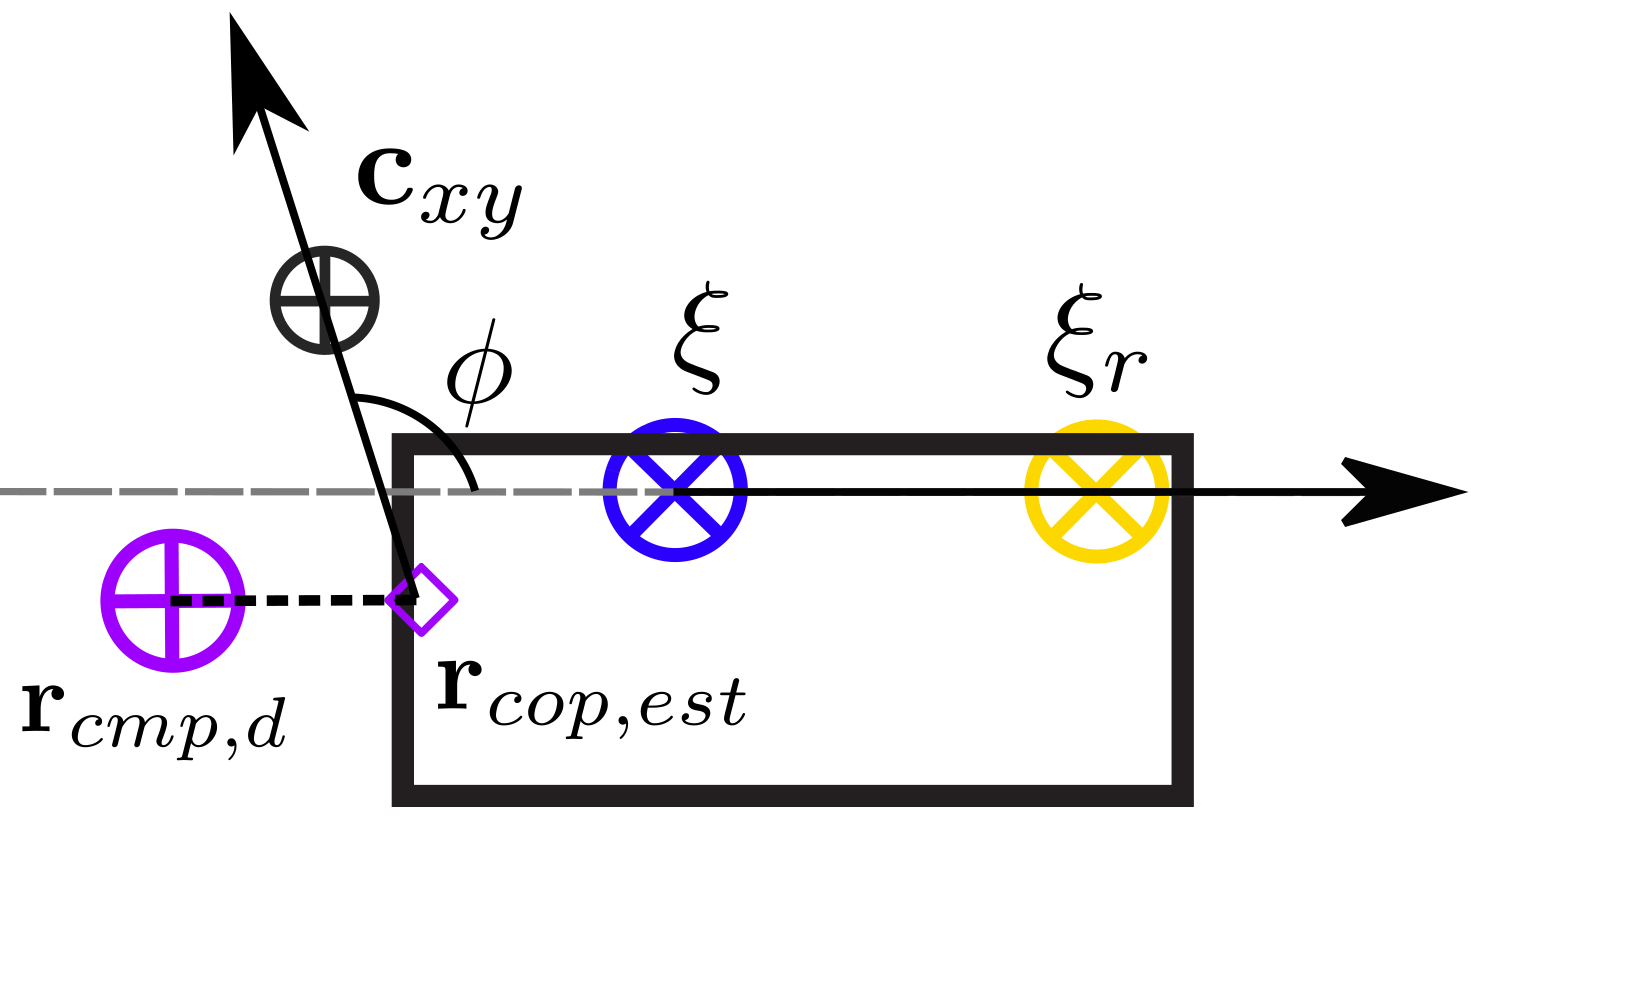
\includegraphics[width=.7\linewidth]{STYLESTUFF/ICPplanStartSSPhiViz.png}
  \caption{}
   \label{fig:phiVizb}
  \end{subfigure}
    \begin{subfigure}{0.49\textwidth}
    \centering
  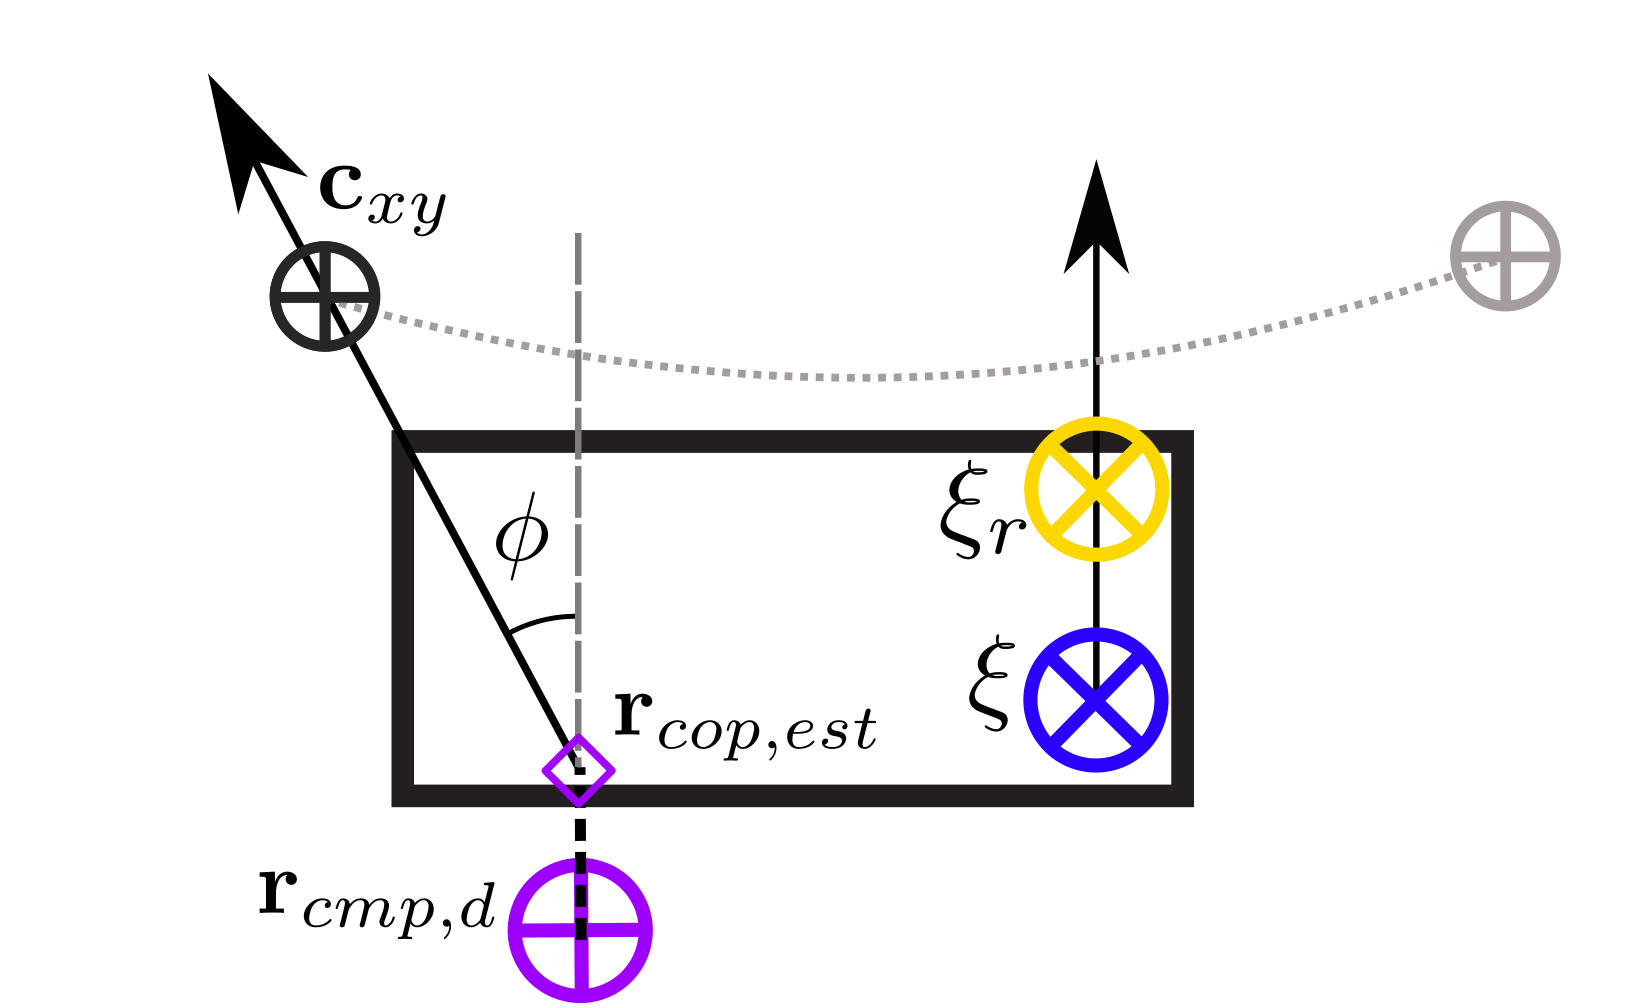
\includegraphics[width=.7\linewidth]{STYLESTUFF/ICPplanStartSSPhiVizLeftError.png}
    \caption{}
     \label{fig:phiVize}
  \end{subfigure}
  \begin{subfigure}{0.49\textwidth}
    \centering
  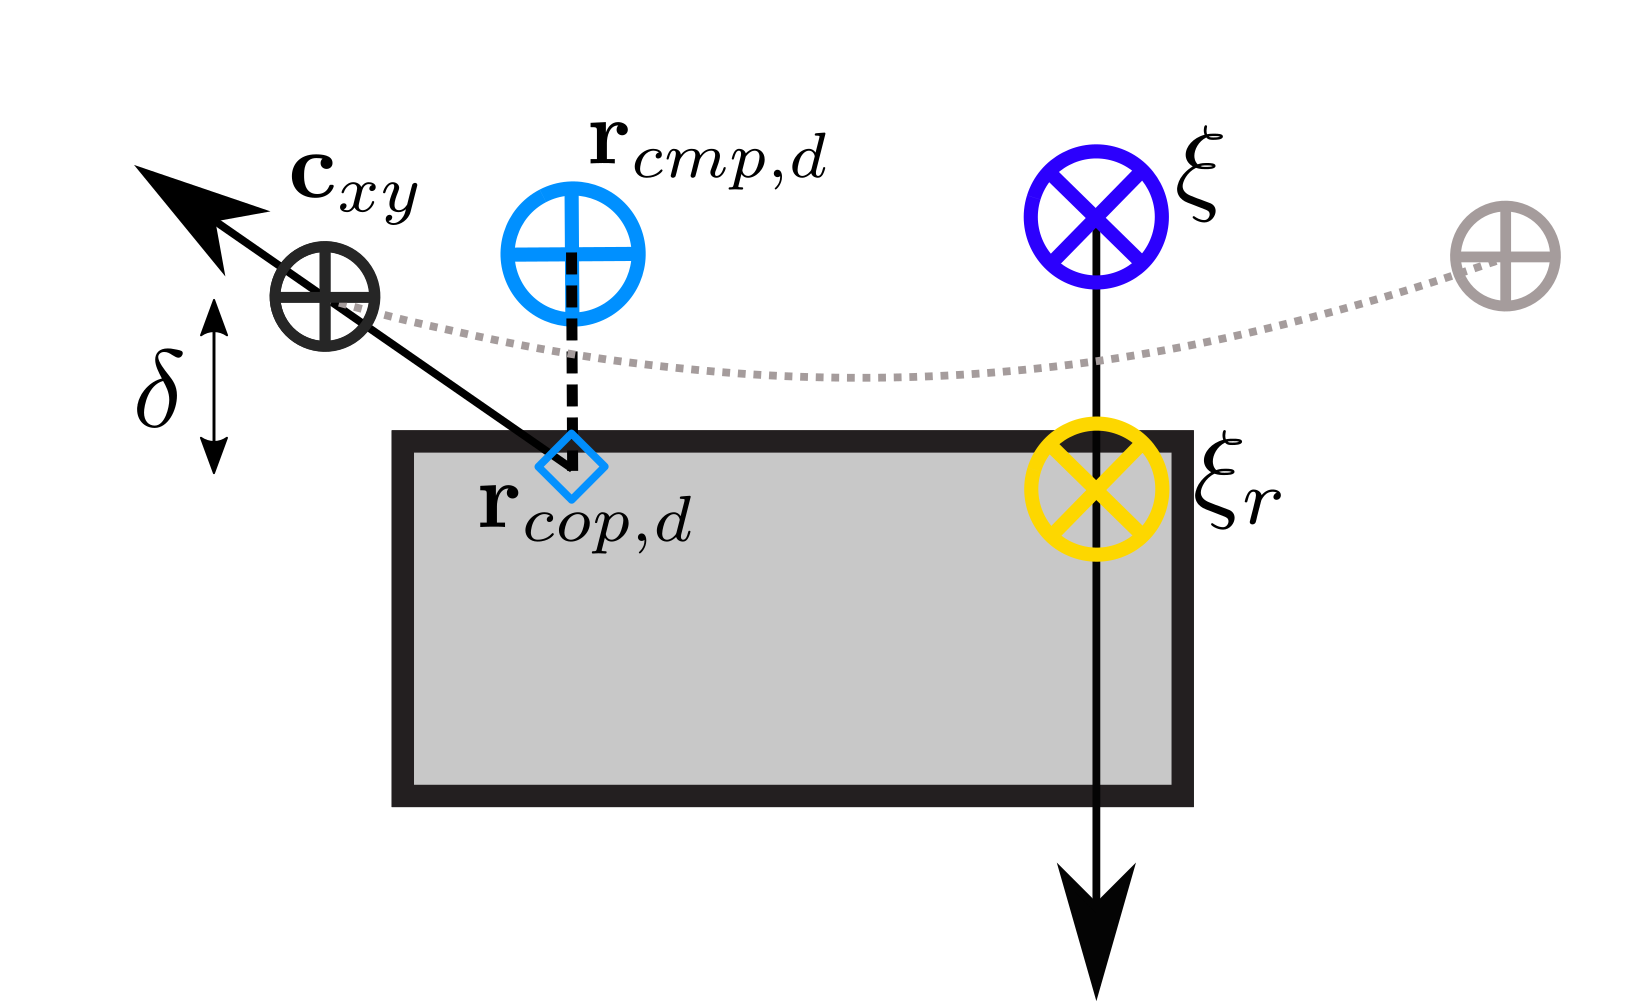
\includegraphics[width=.7\linewidth]{STYLESTUFF/ICPplanStartSSPhiVizRightError.png}
    \caption{}
     \label{fig:phiVizf}
  \end{subfigure}
  \caption{Visualization of $\delta$ and $\phi$ for different error directions. (a) The action `positive alignment' is used. (b) `Prepare' is used. (c) `Positive alignment' is used. (d) `Default' is used.}
  \label{fig:phi}
\end{figure}

For the maximum height constraint $\zmax$, the same parameters as for the standing tests is used in the first half of \ac{SS}. In the second half, the maximum height constraint is linearly interpolated between the maximum height constraint for standing and a maximum height constraint at the end of \ac{SS}.  For the minimum height constraint $\zmin$, a constant value is considered. The height constraints are visually explained in \figref{fig:heightconstraints}.
\begin{figure}
\centering
  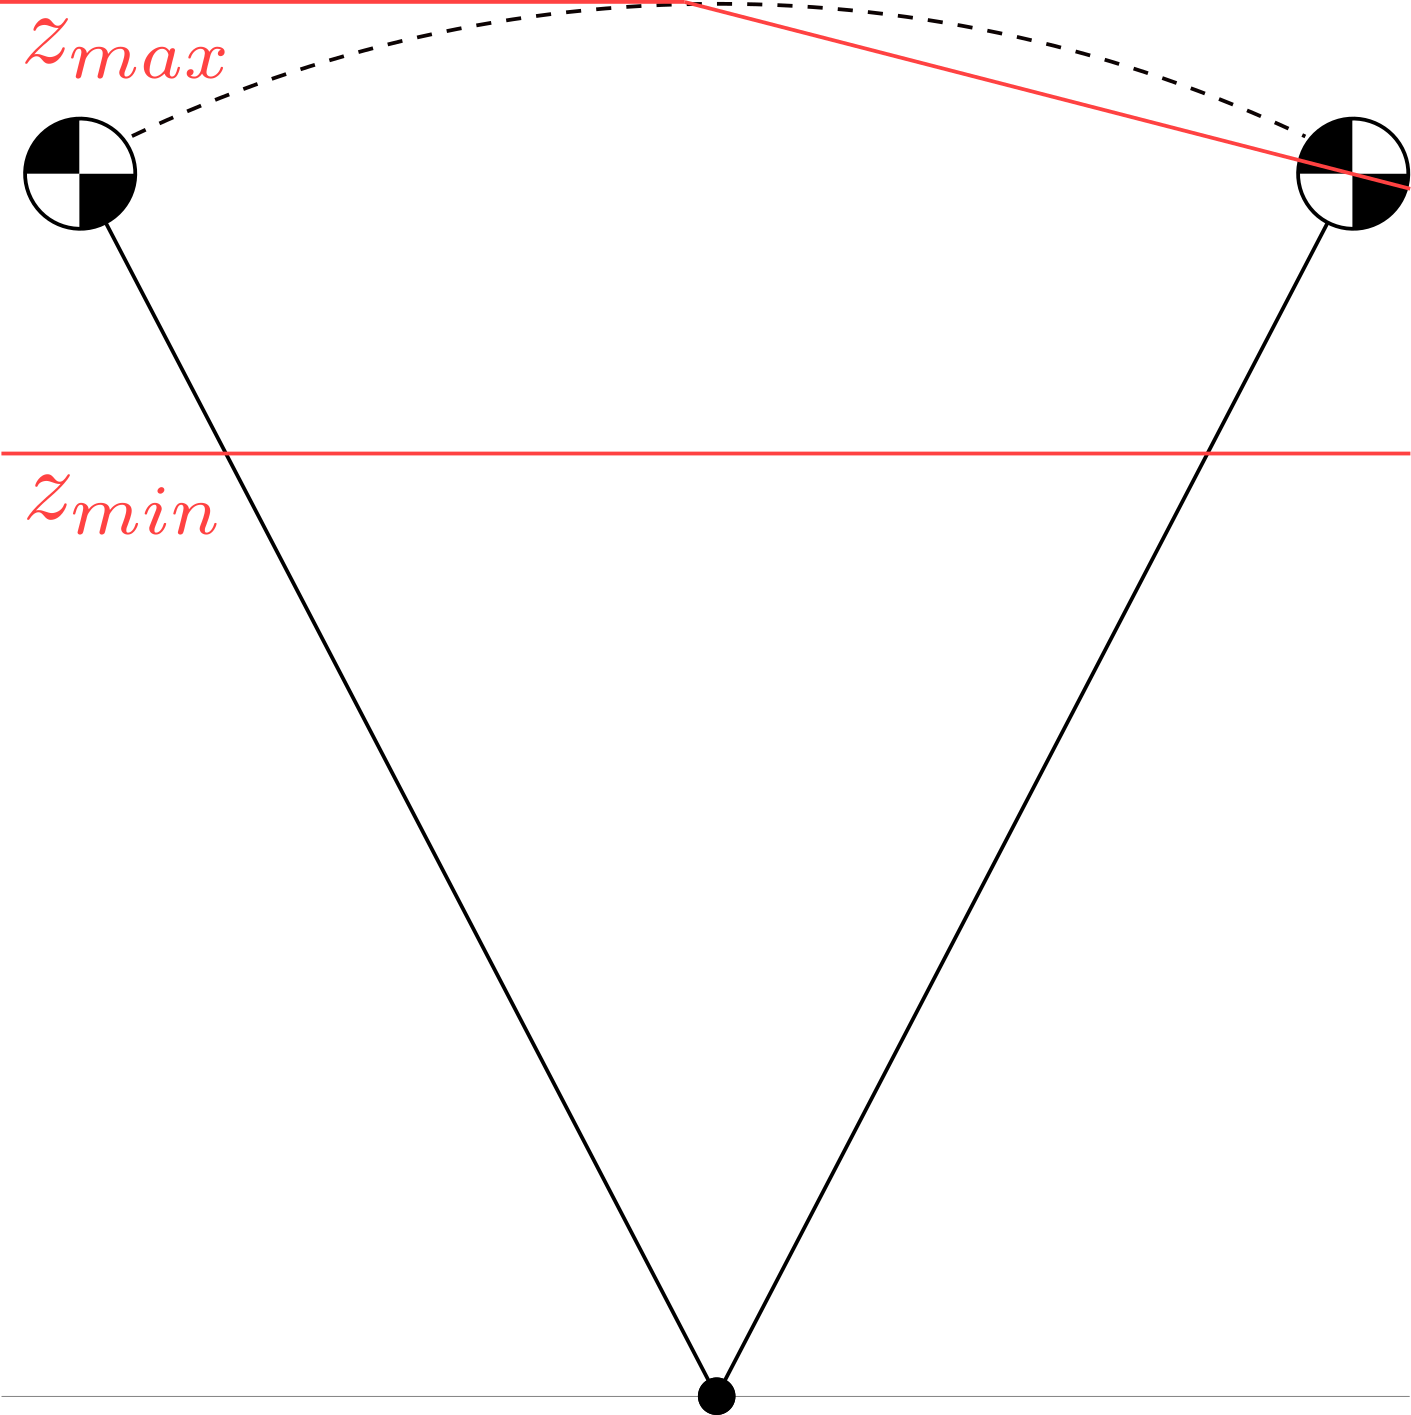
\includegraphics[width=.4\linewidth]{STYLESTUFF/heightconstraints.png}
   \caption{Height constraints through \acf{SS}}
    \label{fig:heightconstraints}
\end{figure} 
\paragraph{The positive alignment action} introduces the bang-bang control law of the previous chapter, using the $\zmax$ as explained above. After the second `bang', the height is not controlled to the maximum height $\zmax$, but is given a feedforward downward acceleration computed with a circle as follows. Consider the distance from the ankle of the robot to the sagittal \ac{CoM} position $x_{ankle}$ and the maximum leg length $l_{max}$. The horizontal position relates to the vertical position as:
\begin{equation}
z^2 = l_{max}^2-x_{ankle}^2.
\end{equation}
The vertical velocity resulting from this function reads as:
\begin{equation}
 \dot{z} = -\frac{x_{ankle}\dot{x}}{\sqrt{l_{max}^2-x_{ankle}^2}}.
\end{equation}
The resulting vertical acceleration reads as:
\begin{equation}
\ddot{z} = \frac{\sqrt{l_{max}^2-x_{ankle}^2}(-\dot{x}^2-x_{ankle}\ddot{x}) - \frac{x_{ankle}^2\dot{x}^2}{\sqrt{l_{max}^2-x_{ankle}^2}}}{ l_{max}^2-x_{ankle}^2}.
\end{equation}
Assuming the sagittal acceleration $\ddot{x}$ is zero, the desired height acceleration is computed as:
\begin{equation}
 \ddzd = -\frac{\dot{x}^2}{\sqrt{ l_{max}^2-x_{ankle}^2}} - \frac{x_{ankle}^2\dot{x}^2}{(l_{max}^2-x_{ankle}^2)^{1\frac{1}{2}}}
\end{equation}
\paragraph{The prepare action} uses the time it takes to accelerate from the minimum height constraint to the maximum height constraint. This time uses the kinetic and potential energy:
\begin{equation}
	\zmin + \frac{1}{2}\ddzc t_{\zmin \rightarrow \zmax}^2 + \frac{1}{2}\frac{(\ddzc t_{\zmin \rightarrow \zmax})^2}{\ddzalpha \ddzc} = \zmax,
\end{equation}
where $t_{\zmin \rightarrow \zmax}$ is the time from the minimum height constraint to the maximum, considering a zero initial vertical velocity.
This solution for the time reads as:
\begin{equation}
 t_{\zmin \rightarrow \zmax}= \sqrt{\frac{2(\zmax - \zmin)}{\ddzc + \frac{\ddzc}{\ddzalpha} }}.
\end{equation}

This time is used to determine the moment when the first `bang' should be activated. The known remaining time in \ac{SS} $t_{r}$ is shortened by $ t_{\zmin \rightarrow \zmax}$:
\begin{equation}
	t_{z \rightarrow \zmin} =t_{r} - t_{\zmin \rightarrow \zmax},
\end{equation}
where $t_{z \rightarrow \zmin} $ is the time available to move from the current height $z$ to the minimum height $\zmin$. Using this time, at every control tick the desired acceleration $\ddzd$ is computed by using the equation:
\begin{align}
	z + \dot{z}t_{z \rightarrow \zmin} + \frac{1}{2}\ddzd t_{z \rightarrow \zmin}^2 - \frac{1}{2}\frac{(\ddzd t_{z \rightarrow \zmin} + \dot{z})^2}{\ddzalpha \ddzc} &= \zmin, \\
	\underbrace{-\frac{1}{2}\frac{t_{z \rightarrow \zmin}^2}{\ddzalpha \ddzc}}_a \ddzd^2 + \underbrace{(\frac{1}{2}t_{z \rightarrow \zmin}^2-\frac{t_{z \rightarrow \zmin}}{\ddzalpha \ddzc} \dot{z})}_b \ddzd + \underbrace{z -\zmin +\dot{z}t_{z \rightarrow \zmin} -\frac{1}{2}\frac{\dot{z}^2}{\ddzalpha \ddzd}}_c&=0,
\end{align}
which has the solution:
\begin{equation}
 	\ddzd = \frac{-b + \sqrt{b^2-4ac}}{2a}.
\end{equation}
This value for $\ddzd$ is used until $t_{z \rightarrow \zmin}<0$, after which the positive `bang' is activated. 

% Results
\section{Results}
The results are obtained by pushing the robot in \ac{SS} when the right foot is the support foot, as in the previous sections. Initially, the robot is pushed at entrance of \ac{SS}. Like with the standing tests, the maximum recoverable push is search for for every $5$ degrees change in push direction, and compared with the default controller. Additionally, pushes are applied in different moments in \ac{SS}, using the notation $\fracpush$ for the fraction of the swing time when the push is applied. To have a more instant change in error, a push duration of $\tpush=0.03$ is chosen. For a more reactive response on Valkyrie, the values $\ddzdmax=5.0$ [m/s$^2$] and $\dddzmax=200$ [m/s$^3$] are chosen to work with.

In \figref{fig:roundPushActions}, the maximum recoverable normalized impulses $i$ are plotted for the different actions together with the results for the default controller. Like with the standing tests, $\rcmpd$ is constrained to be inside the polygon and is assumed to coincide with $\rcopd$. The actions have less effect when the push is applied later in \ac{SS}, and results in even worse recovery than the default setup at $\fracpush=0.5$. Note that the recovery for a push around $200$ degrees is always worse when the vertical motion control law is enabled.
\begin{figure}
     \centering
        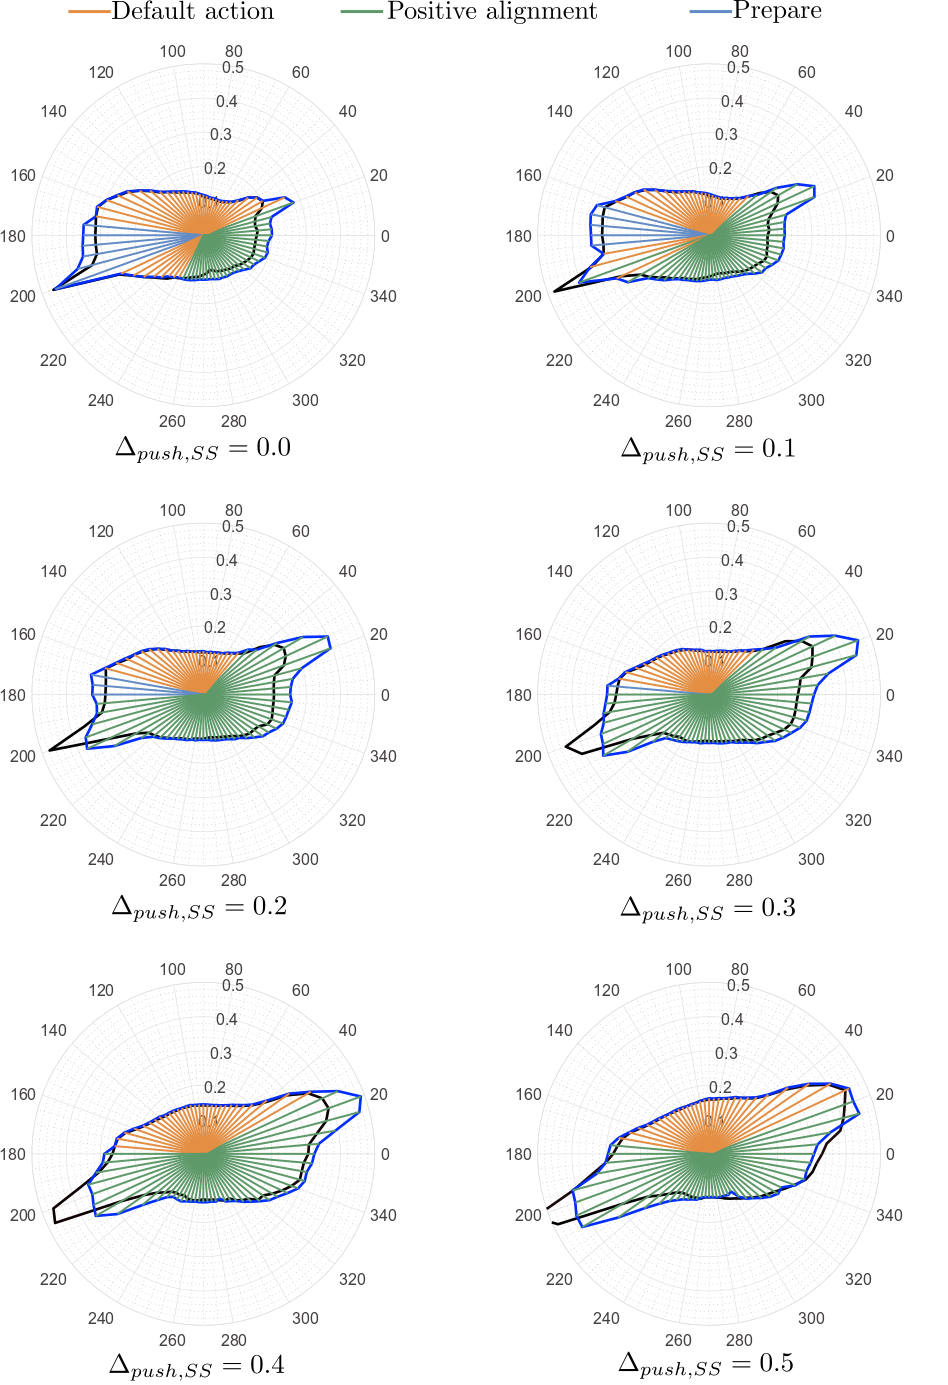
\includegraphics[width=0.85\textwidth]{STYLESTUFF/rounActions.png}
    \caption{Recoverable pushes for the default controller (black) and the vertical motion controller (blue). The radial lines show the actions used by the vertical motion control law.}
    \label{fig:roundPushActions}
\end{figure}

In \figref{fig:roundPushAng}, the maximum recoverable pushes are shown for when $\rcmpd$ is constrained to be inside the polygon, like in the previous figure, and when $\rcmpd$ is allowed to leave the polygon $5$ [cm]. Allowing $\rcmpd$ to go outside the polygon potentially requests angular momentum rate from the robot. However, this is highly dependent on the weights used in the whole-body \ac{QP}. Note how the plots with larger possible $\rcmpd$ locations seem to match shape with the plots where $\rcmpd$ is inside the polygon. Also note how for push directions coming from the back, the recovery is about the same for the default controller with larger $\rcmpd$ locations compared with the vertical motion controller where $\rcmpd$ is constrained to be inside the polygon.
\begin{figure}
     \centering
        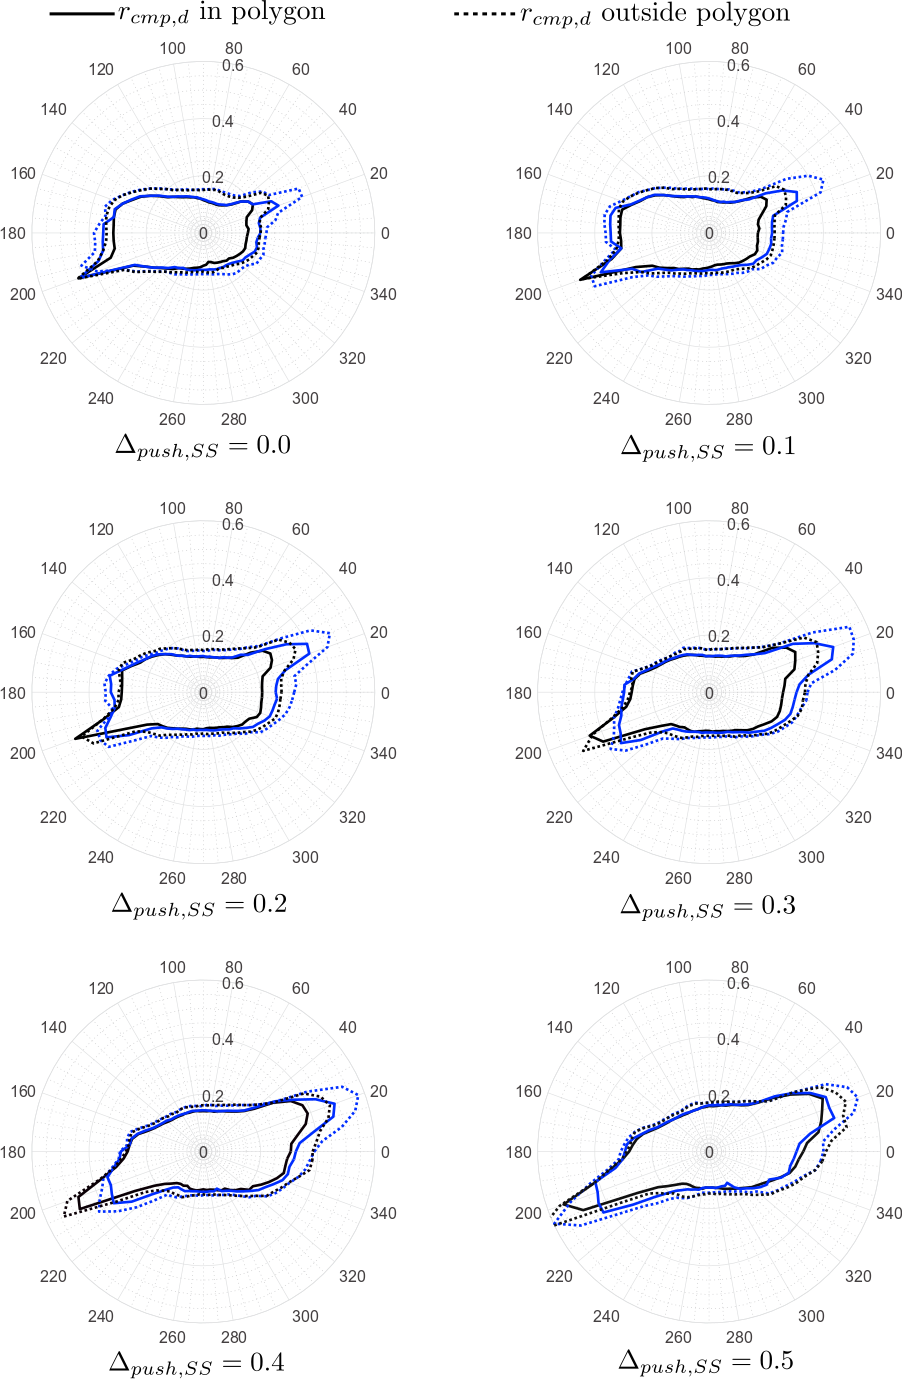
\includegraphics[width=0.85\textwidth]{STYLESTUFF/roundAng.png}
        \caption{Recoverable of the recoverable pushes for the default controller (black) and vertical motion controller (blue). A comparison is shown for when the desired \ac{CMP} is constrained to be inside the polygon, and when the desired \ac{CMP} is allowed to leave the polygon $0.05$ [m].}
        \label{fig:roundPushAng}
\end{figure}
% Discussion
\section{Discussion}
Barely an example.

- Predefined swing time.

- Tuning of thresholds.

- Relying on other control strategies in orthogonal direction. 

- $200$ degree point.

- \ac{CMP} and angular momentum usage.-> bang-bang control \ac{CMP}.

%
% Another appendix chapter
\chapter{Conclusion}\label{chap:conclusion}
The objective of this work was to improve balance control of a humanoid robot using \ac{CoM} height variation. In this work, novel capture regions for the \ac{VHIP} model were proposed and compared with the \ac{LIP} model, which addressed the theoretical part of the research objective. Furthermore, control actions that use \ac{CoM} height variation for balance were presented and results were shown on hardware on humanoid robots in comparison with predefined \ac{CoM} height approaches. For Valkyrie, it was observed that balance was improved using \ac{CoM} height variation, which addressed the applied part of the research objective. 

For the \ac{VHIP} model, capture regions were proposed in Chapter \ref{chap:regions} considering a unilateral contact constraint, after which height constraints and force constraints were added. It was observed that the capture region becomes smaller after addition of constraints. Also, a comparison with the \ac{LIP} and \ac{LIP} plus flywheel capture regions was made, which gives a high-level measure of the potential effects of \ac{CoM} height variation. The presented capture regions were derived under the assumption that kinematic limits and joint torque limits of the robot can be approximated with a constraint on minimum and maximum height and vertical acceleration respectively. 

Because the vertical force constrained capture regions are computed numerically, there was experimented with another control law, a \ac{MPC} law, in Chapter \ref{chap:mpc}. Based on the shape of the control input of the \ac{MPC} however, which is constrained to be a polynomial function, there was chosen to not use this control law in applications in Chapter \ref{chap:standing} and Chapter \ref{chap:walking}.

Similar to the control law used to compute the vertical force constrained capture regions, a bang-bang control law was designed for implementation in a momentum-based whole-body control framework in Chapter \ref{chap:standing}. This control law is activated when a predefined threshold is met. With this control law, push recovery tests were conducted on NASA's Valkyrie and Boston Dynamics' Atlas, while the robots were standing. The results for Valkyrie in simulation showed that push recovery improved $9$\% after pushing the robot in the back and $4$\% after pushing from the side when the bang-bang control law on vertical \ac{CoM} motion was used. Remarkably, push recovery was $7$\% worse after a frontal push when enabling the bang-bang controller. The rear push tests were also conducted on hardware, using a push stick and a load sensor, where an average of $7$\% increase in maximum recoverable push was observed. The vertical force constrained capture position for the same height change and vertical acceleration differed approximately $4$\% from the \ac{CP}, so differences were observed between the \ac{VHIP} model and the results on Valkyrie. Additional hardware tests were also conducted on Atlas with a medicine ball on a rope. However, recovery did not improve noticeably. Different initial heights for the robot were tried, as well as a tuning of a joint torque control gain, which had no effect. In simulation however, recovery did improve when enabling the bang-bang control action.

Similar to the bang-bang control action, three actions were proposed for the use in \ac{3D} in Chapter \ref{chap:walking}. Using the two presented variables, the alignment angle and the effective distance, a control action was chosen heuristically based on outputs of \ac{ICP} control. Compared to a constant height control approach, recovery improved the most when pushing the robot in the back or from the front in the first part of the swing phase. On hardware, evaluation of the proposed control law was difficult, because of the additional uncertainties compared to the standing tests. Therefore, only an example was shown for a control action on hardware on Atlas while the robot is walking.

\section{Recommendations}
The results presented in this work have demonstrated that \ac{CoM} height variations can improve balance control. There are however shortcomings, both on the theoretical as well as the applied side of the proposed research. In the following sections, recommendations for future work are presented. First, recommendations for extension of the proposed approaches are presented, after which a broader outlook on future work is briefly presented.
\subsection{Extending the Proposed Approach }
In this section, opportunities for improvement of the presented theory, tests and results are presented.
\subsubsection{Extension of Capture Regions}
The unilateral contact and height constrained capture regions give bounds on the capture region. However, these cannot directly be used in a control law, as impacts are considered in the computation. The vertical force constrained capture points can be used in control, but use numerical integration to find future state information. It would be interesting to explore closed-form solutions for a force constrained capture problem, without overly constraining the \ac{VHIP} like in \cite{pratt2007derivation} and \cite{koolen2016balance}. With a closed-form solution for example, the control law used in application in this thesis could be predictive, as a vertical force constrained capture position could be computed on every time instance.
\subsubsection{Improving Push Recovery Tests}
Balance control of the robots was tested in this work by testing push recovery. The push stick with load sensor \cite{iload} measures push force accurately, but a person pushing the robot is in general not able to apply a desired force precisely. With the tests with the medicine ball, the ball location could be put relatively precise. However, the push duration on the robot using these tests cannot be adjusted and is quite short, which resulted in high impacts on the robot. Furthermore, stretch in the rope and in the ball can change the \ac{CoM} height of the ball. Also, the transfer of the energy of the ball to the robot depends on the damping properties of the ball and the robot. For future push recovery tests, it could be interesting to use a device that can accurately apply force according to a desired profile over time.
\subsubsection{Improving State Estimation and Center of Pressure Control}
Applying the methods presented in this thesis requires good state estimation and control of the \ac{CoP}. In some experiments on Atlas it was found that performance did not improve when applying the presented control law, even though performance could improve according to the \ac{VHIP} model and the obtained simulation results. This lack of performance could be related to a \ac{CoP} error, which could be caused by the additional movement of the robot when the presented method was used. By improving state estimation and \ac{CoP} control, the theoretically predicted improvements could potentially be better achieved in practice.
\subsubsection{Standing Tests for Lowering Center of Mass Height}
The standing push recovery tests presented in this work all use an increase in \ac{CoM} height for balance control, as the initial \ac{CoM} position of the robot was inside the support polygon at the moment the push was applied. With the walking tests, the \ac{CoM} height was lowered. However, the walking tests were difficult to test on hardware, because of the increased number of uncertainties. It could be interesting to find a test setup, where the robot should lower the \ac{CoM} height to balance to a standing configuration. The robot can be given an initial velocity when the \ac{CoM} is outside the support polygon, that lowering the \ac{CoM} height would be needed to balance. This test setup would be comparable with a human landing after a long jump.
\subsubsection{Analysis of Results}
In this work, the data obtained from the robots was predominantly analyzed based on time response and phase plots. It could be interesting to perform additional analysis, as for example analyzing the energy consumption on the robot when using the different control strategies. The energy consumption could be determined by, for example, measuring the electric current and voltage going to the robot.

\subsection{Outlook}
The work in this report contributes merely a small part to balancing strategies for a humanoid robot. For the future, it could be interesting to analyze \ac{CoM} height variations in legged systems further. It would be interesting to investigate when humans use height variation, and why the strategy is chosen instead of the `hip strategy' in such scenarios for example. Furthermore, it would be interesting to see different balancing strategies combined with height variation on humanoid robots. The decision making in balancing strategies, under the constraints of kinematic limits, force limits, disturbances and terrain remains a broad research area to explore.
%
%
%========================== Appendices =======================================
\appendix
%
%%
% Another appendix chapter
\chapter{Yet Another Appendix}


\section{Test Section (Again?)}

Ok, all is well.


%========================== Back matter ======================================
\backmatter
%
% Bibliography
\bibliographystyle{ieeetr}
\printbib{MyBib}
%
%
% Glossary
\chapter{Glossary} %
%
\printacronyms
\begin{acronym}[\hspace{0.8in}] % 0.8in is also used by the nomenclature
	\acro{3mE}[3\textlarger{m}E]{Mechanical, Maritime and Materials Engineering}%
	\acro{DCSC}{Delft Center for Systems and Control}%
	\acro{ICP}{Instantaneous Capture Point}%
	\acro{CP}{Capture Point}
	\acro{DCM}{Divergent Component of Motion}%
	\acro{ZMP}{Zero Moment Point}%
	\acro{CoP}{Center of Pressure}%
	\acro{CoM}{Center of Mass}%
	\acro{CMP}{Centroidal Momentum Pivot}
	\acro{eCMP}{enhanced Centroidal Momentum Pivot}%
	\acro{VRP}{Virtual Repellent Point}%
	\acro{LIP}{Linear Inverted Pendulum}%
	\acro{2D}{Two-Dimensional Space}%
	\acro{3D}{Three-Dimensional Space}%
	\acro{HZD}{Hybrid Zero Dynamics}%
	\acro{MPC}{Model Predictive Control}%
	\acro{GUI}{Graphical User Interface}%
	\acro{SCS}{Simulation Construction Set}%
	\acro{IMU}{Inertial Measurement Unit}%
	\acro{EKF}{Extended Kalman Filter}%
	\acro{SLIP}{Spring-Loaded Inverted Pendulum}%
\end{acronym}%
%
%
% Nomenclature
\printnomencl%

%
% Index
\cleardoublepage
\printindex

\end{document}
